\documentclass{xduugthesis}
\usepackage{booktabs}
\usepackage{enumitem}
\usepackage{amsmath}
\usepackage{amssymb}
\usepackage{tcolorbox}
\tcbuselibrary{skins,breakable}

\xdusetup{
  style = {
    latin-font = tacn,
    % math-font = termes,
  },
  info = {
    title = {基于深度学习的免疫多肽结合预测\\模型的优化与部署},
    author = {李常凯},
    department = {生命科学技术学院},
    major = {生物医学工程},
    class-id = {2215011},
    student-id = {22159100047},
    % supervisor = {曾文锋},
    supervisor-school = {徐欣怡},
    supervisor-enterprise = {曾文锋},
    bib-resource = {ref.bib},
    % abstract = {chapters/abstract_zh.tex},
    abstract* = {chapters/abstract_en.tex},
    % keywords = {MHC-I 肽段结合预测,模型轻量化,降维,INT8量化,索引检索},
    % keywords* = {MHC-I peptide binding prediction,model lightweighting,dimensionality reduction,INT8 quantization,index retrieval},
    acknowledgements = {chapters/acknowledgement.tex}
    }
  }

% 跳过模板默认封面和中文摘要，仅保留英文摘要、目录和正文。
\ExplSyntaxOn
\cs_set:Npn \__xdu_frontmatter:
  {
    \__xdu_load_main_geometry:
    \pagestyle     { plain }
    \pagenumbering { roman }
    \__xdu_n_chapter_head_ii:nn
      { ABSTRACT } { \rmfamily \zihao { 3 } \bfseries \centering }
    \group_begin:
      \dim_set:Nn \parindent { 2 \ccwd }
      \rmfamily \zihao { -4 }
      \file_if_exist_input:n { \l__xdu_abstract_en_tl }
    \group_end:
    \cs_set:Npn \__xdu_keywords_space: { \hspace { 2em plus 1em minus 1em } }
    \group_begin:
      \rmfamily \zihao { -4 } \bfseries \__xdu_bold_math: \par
      \__xdu_typeout_keywords:nNn
        { Keywords:~ } { \l__xdu_keywords_en_clist } { \__xdu_keywords_space: }
    \group_end:
    \cleardoublepage
    \setcounter { tocdepth } { 5 }
    \__xdu_n_chapter_head:nn
      { \__xdu_lang_switch:nn { 目录            } { Contents } }
      { \__xdu_lang_switch:nn { 目 { \quad } 录 } { Contents } }
    \use:c { @starttoc } { toc }
    \cleardoublepage
  }
\ExplSyntaxOff

% 目录章节标题取消粗体
\renewcommand{\cftchapfont}{\rmfamily\zihao{-4}}
% 目录章节页码取消粗体
\renewcommand{\cftchappagefont}{\rmfamily\zihao{-4}}
% 章节引导点也取消粗体
\renewcommand{\cftchapleader}{\cftdotfill{\cftdotsep}}

\ctexset{
  subsection = {
    afterskip = 0.5\baselineskip
  }
}

\begin{document}

% 临时解决\cite{}没有自动补全提示的问题
% 详见 https://github.com/note286/xduts/discussions/157
\iffalse
  \addbibresource{ref.bib}
\fi


\chapter{绪论}

% \begin{figure}[h]
%     \centering
%     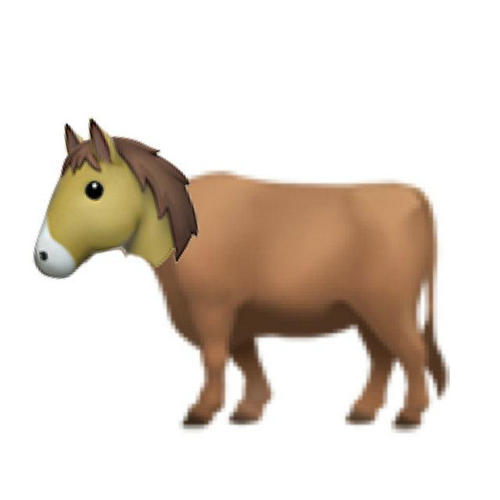
\includegraphics[width=0.5\textwidth]{figures/R-C.jpg}
%     \caption{常见的牛马形象}
%     \end{figure}
    
% \section{研究背景与意义}
% 主要组织相容性复合体（Major Histocompatibility Complex，MHC）分子在适应性免疫应答过程中起着关键作用。其中，MHC-I 分子能够将细胞内来源的肽段递呈至细胞表面，并被 CD8+ T 细胞识别，从而触发后续免疫反应\cite{koh2023cd8}。因此，MHC-I 与肽段的结合能力是抗原递呈过程中的核心环节，围绕 MHC-I 结合肽反应展开预测，也逐渐成为肿瘤新抗原筛选、疫苗设计、免疫治疗和免疫多肽组学等领域的重要研究内容\cite{xie2023neoantigens}。

% 近年来，高通量测序、质谱技术和蛋白质组学研究发展很快，相关的 HLA 及其结合肽数据不断积累，为基于计算方法开展 MHC-I 结合肽预测提供了较好的数据基础\cite{vita2025iedb,thibault2022immunopeptidomics}。与此同时，深度学习在生物信息学中的应用不断拓展，使序列表征能力得到明显提升。相比依赖基序、打分矩阵或浅层机器学习的方法，深度学习模型能够更充分地挖掘 HLA 序列和候选肽段序列中的复杂特征，因此在预测性能和泛化能力上表现出更大优势\cite{lin2023evolutionary,xu2024immuneapp}。

% 将重操作后
适应性免疫应答离不开主要组织相容性复合体（Major Histocompatibility Complex，MHC）分子所发挥的核心功能。其中，MHC-I 分子负责将内源性肽段递呈至细胞表面，供 CD8 T 细胞识别，进而启动下游免疫反应\cite{koh2023cd8}。可见，肽段与 MHC-I 的结合能力是抗原递呈过程中的决定性环节，针对 MHC-I 结合肽的预测研究亦由此在肿瘤新抗原筛选、疫苗设计、免疫治疗与免疫多肽组学等领域占据重要位置\cite{xie2023neoantigens}。

高通量测序、质谱及蛋白质组学技术的快速进步，使得 HLA（同 MHC-I，为同一分子） 及其结合肽数据规模持续扩大，这为基于计算策略的 MHC-I 结合肽预测工作提供了更充实的数据基础\cite{vita2025iedb,thibault2022immunopeptidomics}。同时，深度学习在生物信息学中的渗透程度不断提高，序列表征能力也因此显著增强。相较于依赖基序、打分矩阵或浅层机器学习的原有方法，深度学习模型能够更深入地捕获 HLA 序列与候选肽段序列中的复杂模式，因而在预测准确度与泛化性能上表现出更明显的优势\cite{lin2023evolutionary,xu2024immuneapp}。

在这一背景下，FennOmix.MHC 作为面向 MHC-I 肽段结合预测的深度学习模型，将 HLA/MHC-I 蛋白序列和候选肽段序列作为两个模态输入，通过对比学习将真实结合对在共享嵌入空间中拉近，并将随机负样本推远，从而实现基于距离关系的结合预测与候选筛选。该模型不仅能够完成 MHC-I 肽段结合预测，还具备支持候选肽段检索、缩库辅助搜库等下游任务的潜力，因此具有一定的应用基础。

% 然而，当 FennOmix.MHC 进一步应用到大规模人类蛋白质组场景时，工程部署问题逐渐突出。在典型应用中，需要将人类常见蛋白质序列切分为不同长度的候选肽段，候选规模可达到数千万级。若继续采用原始高维 float32 向量表示，预编码肽段缓存将占用大量存储空间，不仅难以完整放入单块 GPU 显存或普通主机内存中，也会增加磁盘占用、I/O 访问、多进程传输、部署备份和版本管理等方面的压力，最终影响模型在实际环境中的使用效率。

% 将重操作后
然而，将 FennOmix.MHC 推向大规模人类蛋白质组分析时，其工程化部署面临的挑战日益凸显。在典型分析流程中，需先将人类常见蛋白质序列切割成不同长度的候选肽段，候选规模常可达数千万条。若沿用原始的高维 float32 向量表示，预编码肽段缓存将消耗庞大的存储开销：不仅难以整体容纳于单块 GPU 显存或普通主机内存，还会显著加重磁盘占用、I/O 访问、多进程传输、部署备份及版本管理等环节的负担，进而严重制约模型在真实部署环境中的使用效率。

% 从系统角度看，这一问题并不只是“模型参数多”或“单次推理慢”所导致，而是由表示维度、缓存方式、检索流程和运行环境共同形成的综合瓶颈。高维向量会直接增加离线缓存和在线检索成本，频繁的数据加载和跨进程传输又会进一步放大 I/O 压力。同时，模型结构中也可能存在一定冗余，推理过程仍有继续压缩和优化的空间。因此，围绕 FennOmix.MHC 开展轻量化和部署优化，不仅具有明确的工程价值，也具有一定的方法研究意义。

% 与单纯提出新的预测模型不同，本文更关注已有深度学习模型在大规模候选肽段场景中的工程可用性，重点分析模型表示、缓存管理和在线检索之间的协同优化问题。本文围绕 FennOmix.MHC 在大规模人类蛋白质组场景中的部署需求，关注高维缓存、存储开销、I/O 压力和推理冗余等问题，探索兼顾预测性能与工程可用性的优化方案。本文研究意义主要体现在以下三个方面。

% 第一，在理论层面，本文尝试从“表示能力—存储成本—推理效率”的角度分析免疫多肽结合预测模型的部署瓶颈。现有研究通常更关注预测精度，而对模型在大规模候选库场景中的资源消耗讨论相对较少。将轻量化目标纳入模型设计和实验评估，有助于为该类模型的工程化研究提供新的分析视角\cite{li2023model}。

% 第二，在方法层面，本文将模型降维、结构剪枝、缓存量化和索引检索等方法结合起来，尝试形成一套面向部署场景的系统优化思路。该思路并不是单独优化某一个模型指标，而是从模型表示、结构冗余、缓存组织和查询执行多个层面共同降低系统开销，为深度学习模型在免疫多肽结合预测任务中的轻量化应用提供参考。

% 第三，在应用层面，本文研究可为大规模候选肽段筛选、缩库辅助搜库以及资源受限环境下的模型部署提供支持。特别是在真实质谱鉴定场景中，若能将模型预测与数据库检索结合起来，有望减少候选空间规模，降低后续搜库开销，从而增强模型的实际应用价值。

% 综合来看，针对 FennOmix.MHC 在大规模应用场景下面临的部署问题开展系统优化，既具有现实工程意义，也具有一定研究价值。

% 将重操作后
从系统层面审视，该瓶颈并非单纯源于模型参数量大或单次推理耗时，而是由表示维度、缓存策略、检索流程与运行环境共同塑造的复合约束。高维向量直接推高离线缓存与在线检索的开销，频繁的数据加载与跨进程传输则进一步加剧 I/O 负担；同时，模型内部也存在一定的结构冗余，推理链路仍有压缩与加速的余地。正因如此，围绕 FennOmix.MHC 开展轻量化与部署优化，既具备明确的工程价值，也蕴含方法层面的研究意义。

与提出全新预测架构的工作不同，本文更关注现有深度学习模型在大规模候选肽段场景下的工程可用性，重点关注模型表示、缓存管理和在线检索之间的协同优化。围绕 FennOmix.MHC 在人类蛋白质组规模下的部署需求，我们针对高维缓存、存储开销、I/O 压力和推理冗余等瓶颈，探索在保持预测能力的同时提升系统可用性的优化方案。其意义主要体现在三个方面。

在理论层面，本文从“表示能力—存储成本—推理效率”这三者的关系出发，重新审视免疫肽结合预测模型在部署中的瓶颈。目前多数工作仍聚焦于预测精度，对模型在大规模候选库下的资源消耗关注相对较少。将轻量化目标提前纳入模型设计和实验评估，有可能为该类模型的工程化研究提供一种不同于精度竞赛的分析视角\cite{li2023model}。

在方法层面，本文尝试融合模型降维、结构剪枝、缓存量化和索引检索等策略，形成一套面向部署的系统优化思路。这些手段并不追求某一指标的极致，而是从表示、结构、存储和查询四个环节同步降低开销，从而为深度学习免疫肽结合预测模型的轻量化落地提供方法参考。

在应用层面，所得方案可直接用于大规模候选肽段筛选、缩库辅助搜库以及资源受限环境下的模型部署。特别是在实际质谱鉴定流程中，如果将模型预测与数据库检索对接，就有可能先一步缩小候选空间，降低下游搜库的计算成本，明显增强模型在真实业务链路中的实用价值。

概括而言，针对 FennOmix.MHC 在大规模应用中所暴露的部署难题进行系统优化，不仅具有明确的工程落地意义，也具备一定的研究讨论价值。

\section{国内外研究现状}

\subsection{MHC-I 肽段结合预测研究进展}

MHC-I 与肽段的结合预测是免疫信息学的核心问题之一。早期方法主要依靠结合基序、位置特异性打分矩阵和浅层统计学习模型，通过肽段关键位置上的氨基酸偏好来推断与 MHC 分子的结合可能\cite{peters2005generating}。在数据量较小时，这类方法有一定实用性，但面对多样的等位基因、变化的肽长以及跨数据集泛化要求，其局限就变得相当突出。

进入机器学习与深度学习阶段后，该领域逐步从手工构造特征转向数据驱动的表示学习。当前较有代表性的模型包括 NetMHCpan\cite{reynisson2020netmhcpan}、MixMHCpred\cite{gfeller2023mixmhcpred}、ESM 系列\cite{rives2021biological} 和 FennOmix.MHC 等。文献调研显示，NetMHCpan 将短肽序列与 HLA 伪序列一并送入神经网络，并利用基序去卷积框架来改善对不同等位基因和肽长的适应能力；MixMHCpred 直接基于质谱鉴定的 HLA 结合肽，通过基序去卷积学习等位基因特异的位点概率矩阵和肽长分布；ESM 系列则借助海量蛋白质序列的预训练获得氨基酸的通用表示，为下游表位预测提供较高质量的嵌入特征。

与上述方法不同，FennOmix.MHC 采用了双模态编码和共享嵌入空间的设计，将 HLA/MHC-I 蛋白序列和候选肽段映射到同一表示空间，并通过深度对比学习拉近正样本对、推远负样本对。这一思路不仅适用于结合预测，也自然兼容候选肽段检索、数据库缩减和辅助搜库等任务，在功能延展性上具备一定优势。

整体来看，MHC-I 肽段结合预测已经形成了较为多元的方法体系，研究的重心也从单纯追求精度，逐步延伸到更强的表示能力、更好的跨等位基因泛化性以及更贴近真实应用场景的任务适配性\cite{reynisson2020netmhcpan,gfeller2023improved,abelin2024innovations}。不过，相比于模型性能的持续提升，围绕大规模候选肽库场景下的资源消耗和系统部署问题，现有的讨论还比较薄弱。

\subsection{深度学习模型轻量化与部署优化研究现状}

深度学习模型从实验环境走向实际部署，轻量化是不可回避的一步。模型规模持续膨胀所带来的参数量、存储成本、推理延迟和部署复杂度，已经成为制约应用落地的主要瓶颈。针对这些问题，降维、剪枝、量化、知识蒸馏等策略得到了广泛研究\cite{li2023model,cheng2024survey}。

在特征表示层面，降维是一种直接且有效的压缩方式。压缩嵌入向量的维度可以缩减缓存占用，并降低后续相似度计算与检索的时空开销。不同降维方法在压缩率、信息保真度和训练稳定性之间各有取舍：线性方案结构简单、参数量少，非线性方案则在保留复杂特征结构上具备理论优势\cite{sorzano2014survey,wang2016autoencoder}。

在模型结构层面，剪枝是去除冗余参数、减轻推理负担的常用手段。对于 Transformer 类模型，常见的剪枝目标包括注意力头和前馈网络的隐藏单元。通过评估各组件的重要性并裁剪贡献较低的部分，可以在不明显损害模型性能的前提下有效压缩结构复杂度\cite{michel2019sixteen,lagunas2021block}。

在缓存和部署层面，量化是压缩模型参数与向量存储体积的重要技术。将 float32 表示转换为 INT8 等低位宽格式，能显著缩减存储空间和数据搬运开销，但需要留意量化误差对后续检索和匹配环节的影响。另外，在大规模候选向量检索任务中，索引机制同样是部署优化不可忽视的一环。利用预计算缓存并配合哈希映射或向量索引结构，可以避免重复编码与无效遍历，从而提升在线查询的响应效率。

总体而言，轻量化与部署优化技术在通用深度学习领域已有较多探索，但以系统化的方式将它们引入免疫多肽结合预测模型的工作仍不多见，尤其是与大规模候选肽段缓存和下游缩库搜库等任务深度绑定的研究更为稀缺。这恰好为本文以 FennOmix.MHC 为对象，系统开展轻量化与部署优化留出了研究空间。

\subsection{现有工作存在的不足}
尽管 MHC-I 肽段结合预测方法在模型结构和预测精度上已取得长足进步，但从工程部署和应用落地的视角审视，仍存在若干短板。

其一，已有研究大多将提升预测精度作为首要目标，对模型在大规模实际场景中的资源消耗缺少系统性的剖析。面对数千万量级的候选肽段，高质量嵌入仅是必要条件，缓存体量、存储成本与加载效率同样决定着系统能否真正上线。

其二，模型优化与系统优化常被分开讨论。单纯压缩模型参数未必能解决高维缓存问题，单纯缩减缓存也未必能保住表示质量。因而，有必要将编码维度选择、模型结构压缩、缓存格式改造与检索流程设计统筹起来，形成面向部署的整体优化方案。

其三，现有轻量化研究大多缺少与真实下游任务打通的评价体系。对于免疫多肽结合预测模型，常规召回指标仅反映测试集上的表现，难以直接说明其在真实质谱搜库或大规模候选筛选中的实际价值。因此，有必要将轻量化方案与下游任务评价紧密挂钩，从预测效能、候选库保持能力和系统资源开销等多维视角综合判断方案的有效性。

基于以上不足，本文选取 FennOmix.MHC 作为具体研究对象，从表示压缩、结构轻量化、缓存压缩和索引检索等方面入手，尝试构建一套面向实际部署的系统优化方案。

\section{本文主要研究内容}

围绕 FennOmix.MHC 在大规模人类蛋白质组应用中遇到的高维缓存膨胀、推理开销偏高和部署困难等问题，本文从模型轻量化与系统工程优化两个方面展开，具体工作如下。

\begin{enumerate}[label=（\arabic*）, leftmargin=5em, itemsep=0pt, topsep=0pt]
    \item 搭建 FennOmix.MHC 基础实验环境，完成原模型复现。
    \item 探索模型输出维度的压缩方案，评估不同嵌入大小对性能与存储的影响。
    \item 对比线性和非线性降维策略，选取适合部署的默认设置。
    \item 分析模型结构冗余，寻找可行的剪枝路径。
    \item 设计面向肽段缓存的量化压缩方法，缓解存储和加载压力。
    \item 构建大规模肽段索引与在线查询流水线，提升筛选效率。
\end{enumerate}

通过以上工作，本研究试图为 FennOmix.MHC 构建一套面向实际部署的优化方案，在保持较高预测能力的同时，显著压缩存储与推理开销，进而增强其在大规模肽段筛选和下游搜库任务中的实用性。整体技术路线如图~\ref{fig:tech-route}所示。

\begin{figure}[htbp]
\centering
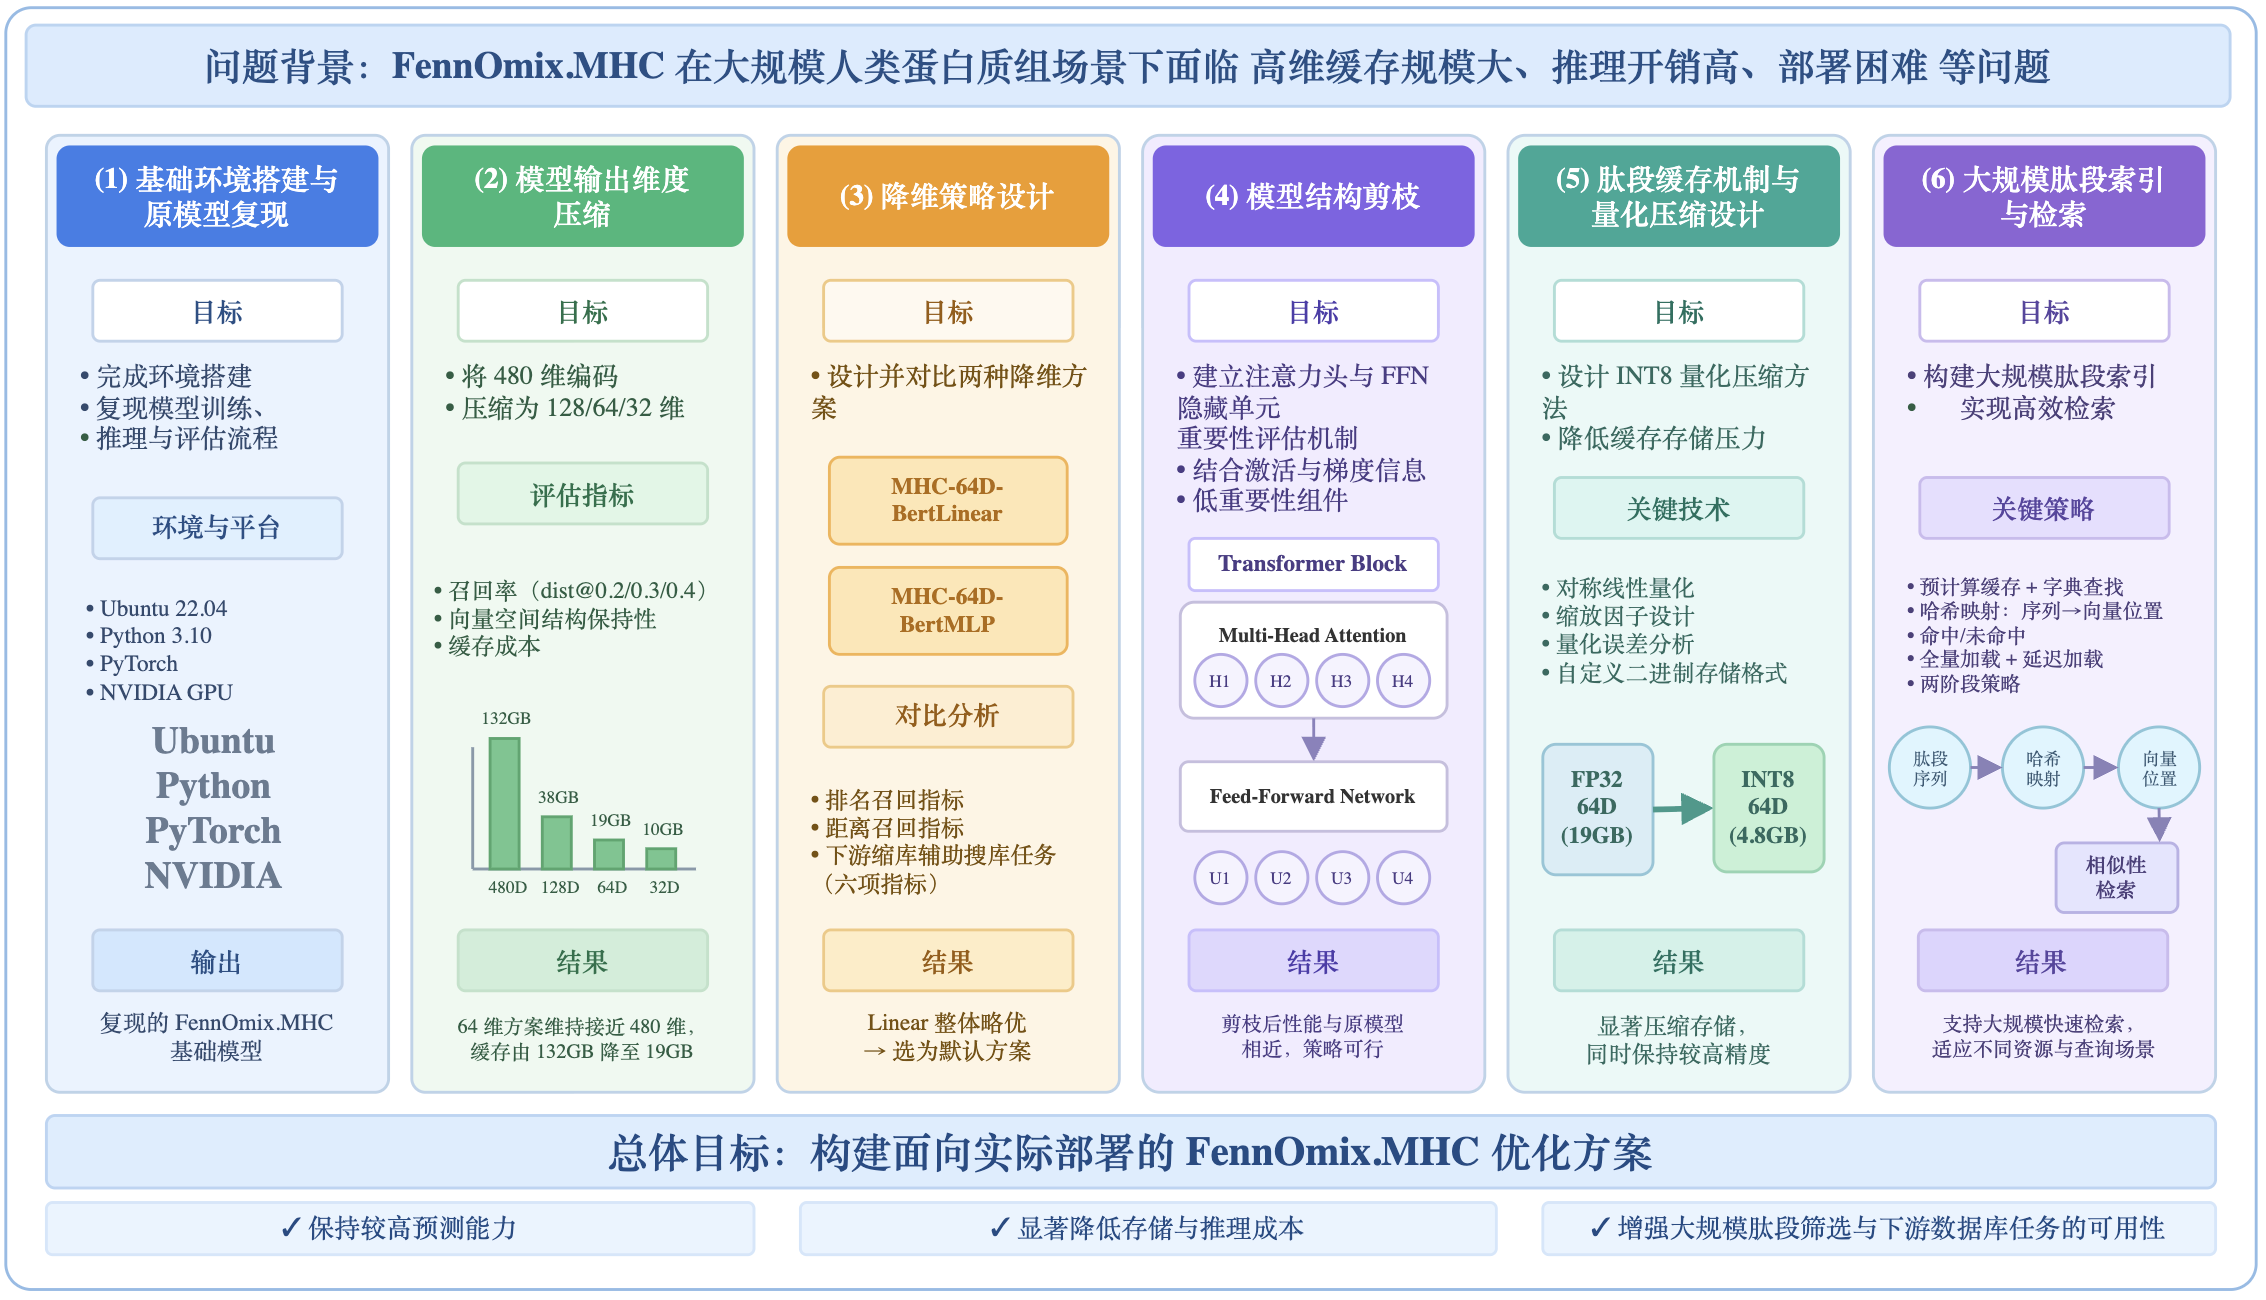
\includegraphics[width=1.0\textwidth]{figures/1.研究技术路线图.png}
\caption{模型优化与部署分析的研究技术路线图}
\label{fig:tech-route}
\end{figure}

% \section{本课题创新点}

% 结合已有研究基础和本文实际开展的工作，本课题的主要创新点概括如下。

% \begin{enumerate}[label=（\arabic*）, leftmargin=5em, itemsep=0pt, topsep=0pt]
%     \item 从实际部署需求出发，对 MHC-I 肽段结合预测模型进行轻量化研究。
%     \item 将表示压缩效果与下游缩库任务性能联动评价。
%     \item 在 FennOmix.MHC 的部署优化中引入结构冗余分析。
%     \item 构建模型优化与缓存、索引机制协同的部署流程。
% \end{enumerate}

\section{论文结构安排}

全文共分五章，具体安排如下。

第一章是绪论，介绍研究背景与意义，梳理国内外研究现状和现存问题，并明确本文的研究内容、创新点及整体结构。

第二章为理论基础与方法设计，将相关理论、模型轻量化策略和缓存索引机制整合论述。该章先交代MHC-I肽段结合预测任务、FennOmix.MHC基本框架、对比学习思想、评价指标以及缩库辅助数据库检索的基础，再围绕模型输出维度压缩、Linear与MLP降维方案、结构剪枝、INT8缓存压缩、自定义二进制格式、哈希索引和在线查询流程展开方法设计。

第三章是实验设计与结果分析，从实验环境、评价方法、不同输出维度比较、Linear与MLP模型对比、剪枝实验以及缓存压缩与索引机制效果等方面进行系统评估。

第四章为系统设计与部署分析，阐述轻量化模型、压缩缓存、索引检索与在线预测模块协同工作的整体流程，并分析系统在实际资源环境中的部署特征。

第五章是总结与展望，归纳全文工作，指出当前研究的局限，并对未来可进一步探索的方向进行展望。

\section{本章小结}

本章阐明了MHC-I肽段结合预测任务的背景与应用价值，分析了FennOmix.MHC在大规模候选肽段场景下所面临的高维缓存压力、存储开销和部署难题；继而回顾了相关研究进展与存在的短板，明确了本文的核心研究内容、创新点及章节安排。后续各章将在此基础上，依次推进模型轻量化、缓存压缩和系统部署优化等工作。

\chapter{理论基础与方法设计}

\section{免疫多肽结合预测任务基础}

\subsection{MHC-I分子与抗原递呈过程}

主要组织相容性复合体在抗原递呈和免疫识别中扮演关键角色。MHC-I 分子普遍存在于有核细胞表面，负责将胞内蛋白降解产生的短肽呈递到细胞表面，供 CD8+ T 细胞识别。在人体中，MHC-I 分子通常对应人类白细胞抗原（Human Leukocyte Antigen，HLA）I 类分子。

抗原递呈过程中，胞内蛋白先被蛋白酶体降解为短肽片段，接着部分肽段进入内质网并与 MHC-I 分子结合，形成稳定的 MHC-I–肽段复合物。该复合物被转运至细胞表面后，可被 T 细胞受体识别，进而参与下游免疫应答。由此，肽段能否与特定 MHC-I 分子稳定结合，便成为抗原递呈与免疫识别的核心环节。

从计算视角看，MHC-I 肽段结合预测的本质是：给定 HLA 分子序列与候选肽段序列，判断二者能否稳定结合，并进一步估计结合强度或优先级。该任务既是抗原递呈研究的基础问题，也是肿瘤新抗原筛选、免疫治疗、疫苗设计和免疫多肽组学分析的重要一环。

\begin{figure}[htbp]
    \centering
    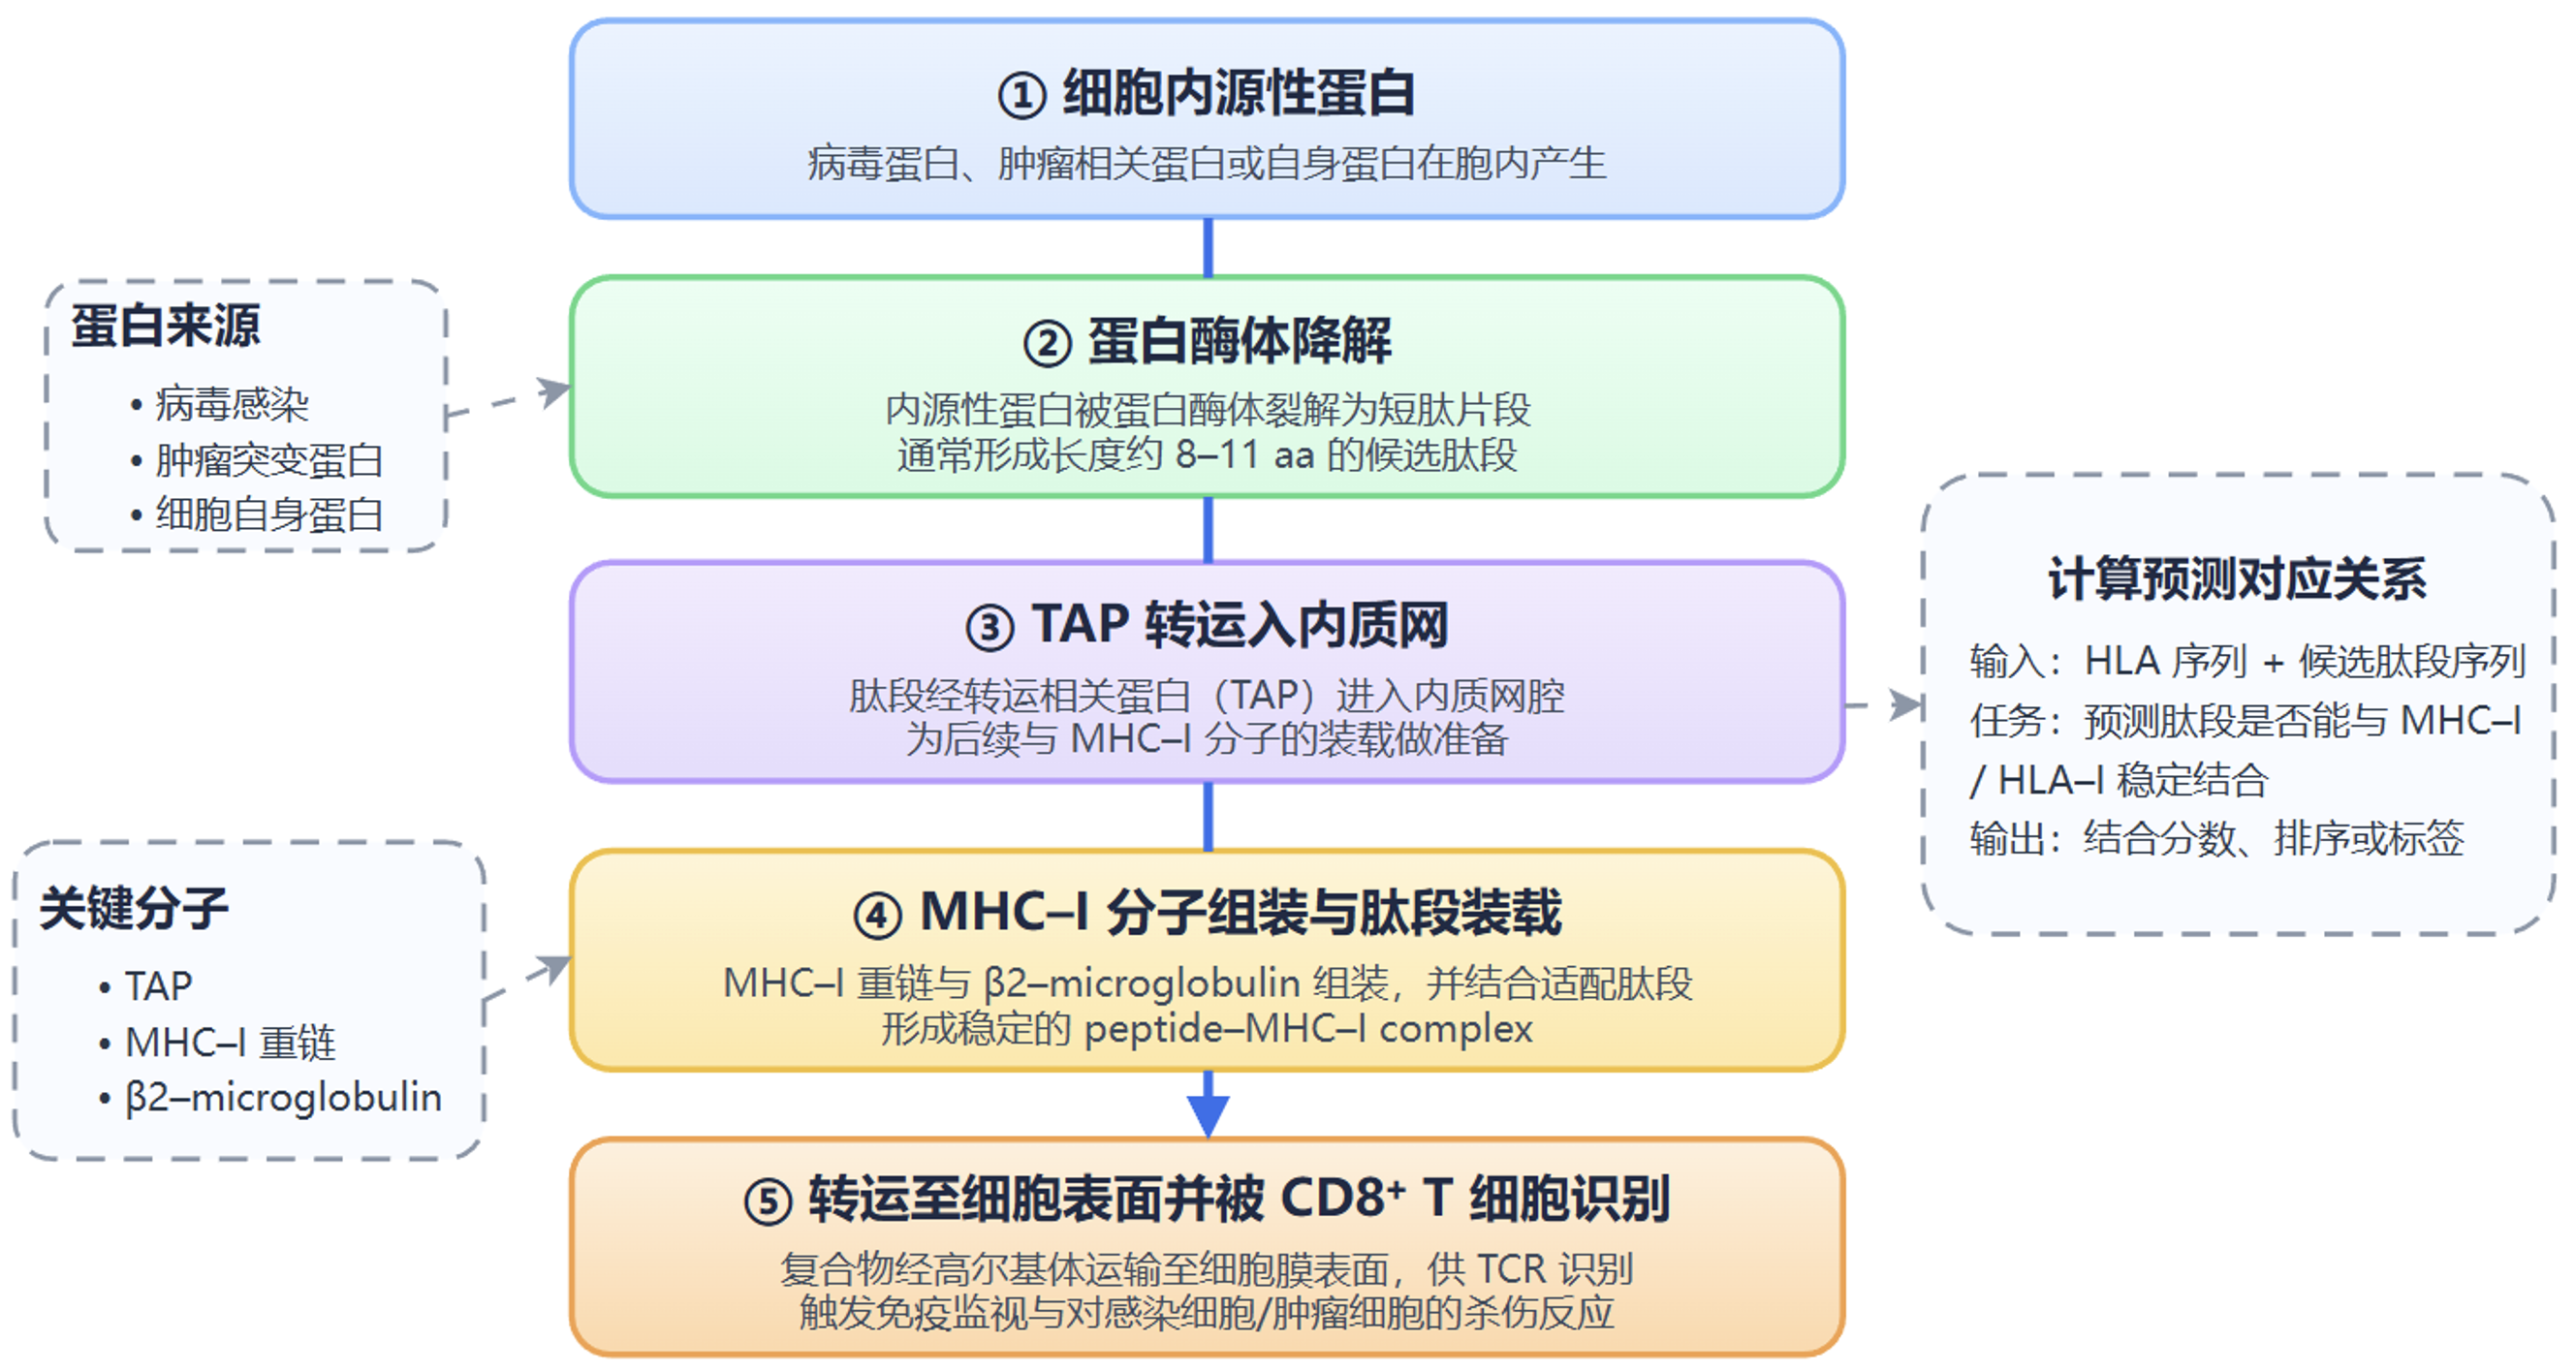
\includegraphics[width=0.85\textwidth]{figures/MHC-I-抗原递呈过程示意图.png}
    \caption{MHC-I 抗原递呈过程示意图}
    \label{fig:MHC-Peptide}
\end{figure}

\subsection{HLA等位基因多态性与预测难点}

MHC-I 肽段结合预测的挑战首先来自 HLA 分子的高度多态性。不同等位基因在结合槽结构、关键氨基酸位点和理化性质上的差异，导致其各自具有不同的肽段锚定位点偏好和长度分布偏好。这意味着同一条肽段在不同 HLA 背景下可呈现完全不同的结合能力，而同一 HLA 分子对长度、组成各异的肽段也具有选择性。

其次，肽段序列的表示本身具有复杂性。虽然 MHC-I 结合肽通常长度较短，但其局部氨基酸组合、位置依赖关系以及与 HLA 结合槽的匹配模式并非简单的线性关系。依赖结合基序、位置特异性打分矩阵或浅层机器学习的方法，在复杂等位基因背景和大规模候选肽段面前，表达能力和泛化能力往往受限。

最后，真实应用场景中的预测任务通常不是对少量候选肽段进行二分类判断，而是需要在大规模候选空间中快速筛选与排序。因此，一个具有实际应用价值的模型不能仅追求预测精度，还必须兼顾计算效率、存储成本和部署可行性。

\subsection{免疫多肽结合预测的任务形式}

从建模角度看，MHC-I 肽段结合预测常见的任务形式主要有两类。第一类是分类或回归式预测，即直接判断结合或估计结合强度。第二类是表示学习式预测，将 HLA 与肽段分别映射至统一向量空间，通过距离或相似度完成匹配、排序和检索。

与传统分类框架相比，表示学习式方法不仅能完成结合预测，还能天然支持大规模候选肽段筛选、向量检索和下游数据库缩减，因此在需要处理海量候选肽段的工程场景中扩展性更强。

本课题研究的 FennOmix.MHC 属于表示学习式方法。该模型以 HLA/MHC-I 蛋白序列和候选肽段序列作为两个模态输入，分别编码为向量，并在共享嵌入空间中通过距离关系刻画两者的匹配程度，从而实现结合预测和候选筛选。

\section{FennOmix.MHC模型与表示学习基础}

\subsection{FennOmix.MHC基础框架}

FennOmix.MHC 是面向 MHC-I 肽段结合预测的深度学习模型，其核心是将 HLA/MHC-I 蛋白序列与候选肽段序列视为两个模态，分别编码至共享嵌入空间。在该空间中，真实结合的 HLA–肽段样本对彼此靠近，而非结合或随机配对样本则相互远离。

相比于直接建模为分类任务，双编码器加共享空间的设计具有两方面优势。其一，模型可分别学习 HLA 与肽段的序列表示，再通过统一度量完成匹配，有助于增强对不同等位基因和不同肽段分布的泛化能力。其二，共享嵌入空间天然适合候选肽段检索、相似度排序和缩库辅助搜库等任务，因而更契合大规模工程应用场景。

\begin{figure}
    \centering
    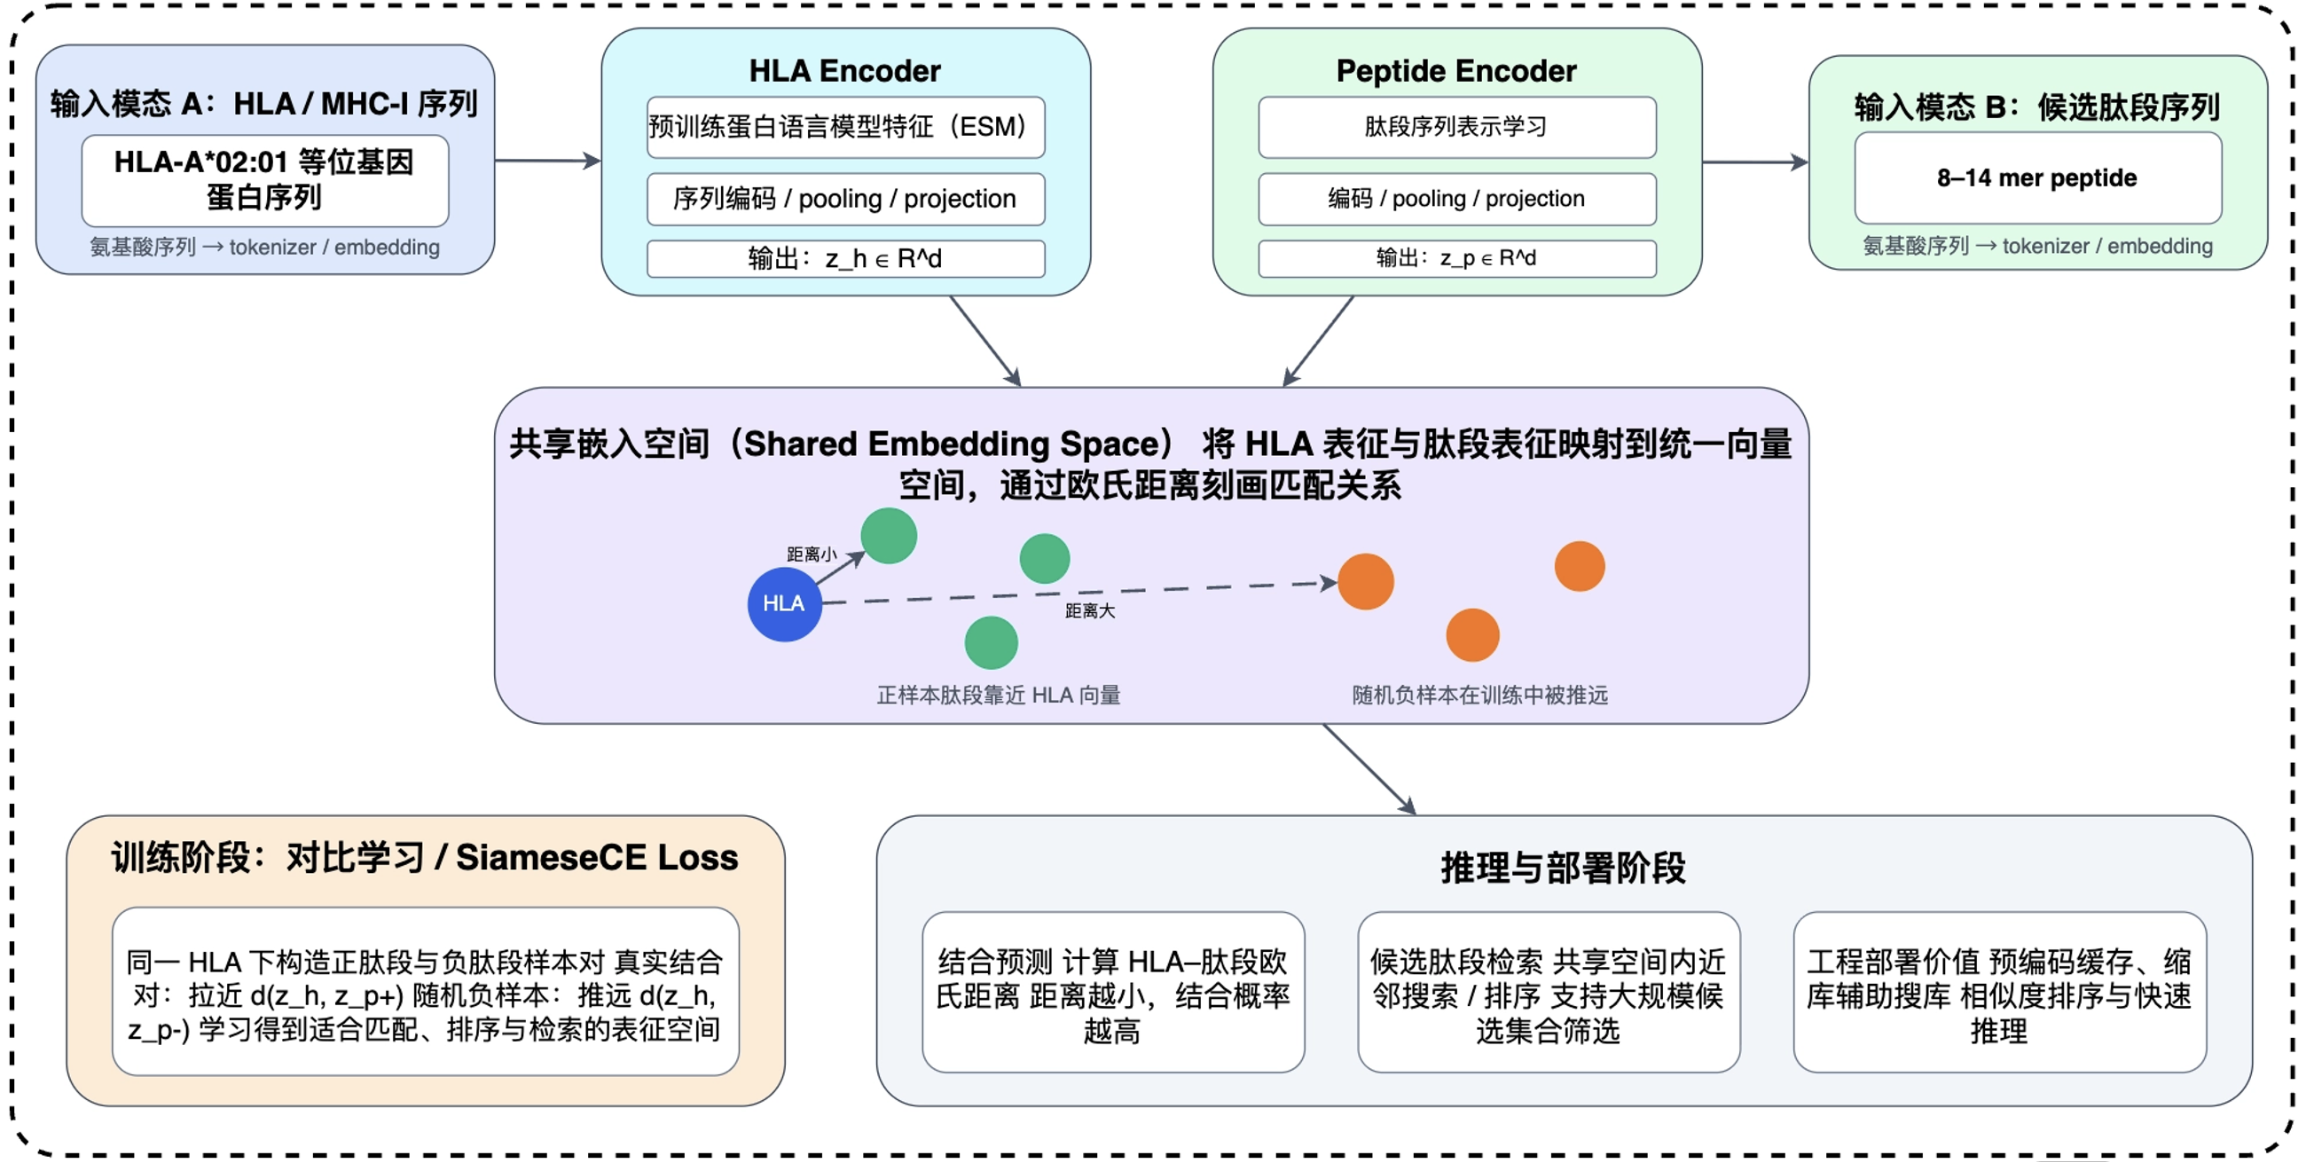
\includegraphics[width=1.0\textwidth]{figures/FennOmix.MHC 基础框架图.png}
    \caption{FennOmix.MHC 基础框架图}
    \label{fig:fennomixmhc-framework} 
\end{figure}

\subsection{输入表示与双模态编码}

FennOmix.MHC 的输入包含两部分：HLA/MHC-I 蛋白序列与候选肽段序列。模型将这两类氨基酸序列编码为向量，供后续相似度计算与匹配预测使用。在后续降维设计中，HLA 编码器以 ESM2 产生的 480 维 token 表示作为上游输入，并进一步通过线性映射或 MLP 进行维度压缩，可见该模型的基础编码阶段已具备较强的预训练表示背景。

从表示学习角度看，双模态编码的本质是在两个输入空间分别提取结构与语义特征，并将其映射至统一语义空间。对 HLA 分子而言，模型需捕获其结合槽相关的序列特征；对肽段而言，则需学习与锚定位点、长度偏好和整体结合模式相关的表示。二者共同决定了后续距离度量的有效性。

\subsection{对比学习与嵌入空间度量}

对比学习的核心在于通过构造正样本对与负样本对，学习一个能够在表示空间中区分它们的映射函数。理想情况下，正样本对在空间中彼此靠近，负样本对则相互远离。在 MHC-I 肽段结合预测任务中，可把真实结合的 HLA–肽段组合视为正样本对，随机配对或 decoy 构造视为负样本对。

与传统监督分类不同，对比学习更关注样本间的相对关系，而非类别标签本身。这种特性使其尤其适合匹配、检索和排序类任务。在很多实际场景中，模型最终并不需要只输出“结合”或“不结合”，而是要在大量候选肽段中给出可靠的相对优先级排序。由对比学习构建的嵌入空间，恰好能够天然支撑这类需求。

共享嵌入空间采用欧氏距离衡量 HLA 与肽段嵌入的匹配程度。肽段嵌入与目标 HLA 嵌入之间的欧氏距离越小，表明该肽段越有可能属于该 HLA 的潜在结合肽段；距离越大，匹配可能性越低。

从表示学习角度看，一个有效的嵌入空间不仅要求正负样本可分，还要求空间结构具备较好的稳定性。当模型经历降维、剪枝或量化等优化操作后，如果向量邻域关系仍能基本保持，就说明原始语义空间没有发生明显扭曲。因此，评价嵌入空间结构是否稳定，是本文后续模型轻量化和缓存压缩研究的重要依据。

\section{评价指标与下游检索任务}

\subsection{基于排名阈值的召回率}

基于排名阈值的召回率用于考察真实结合肽段能否进入模型排序结果的前列。本文使用 rank@0.1、rank@0.5 和 rank@2.0 三个指标，分别统计真实阳性样本出现在预测排名前 0.1\%、0.5\% 和 2.0\% 候选中的比例。

设测试集中 HLA 等位基因集合为 $H$。对于某一等位基因 $h \in H$，其候选肽段集合记为 $C_h$，真实结合肽段集合记为 $P_h$。模型对 HLA 嵌入与肽段嵌入计算欧氏距离，距离越小代表模型判定该肽段与该 HLA 结合的可能性越大。肽段 $p$ 与 HLA $h$ 的距离为：
\begin{equation}
    d(h,p)=\left\|z_h-z_p\right\|_2
\end{equation}
其中，$z_h$ 和 $z_p$ 分别为 HLA 和肽段的嵌入向量。

对所有候选肽段按距离从小到大排序后，肽段 $p$ 在候选集合 $C_h$ 中的排名可表示为：
\begin{equation}
\operatorname{rank}_h(p)
=
1+
\sum_{q \in C_h}
\mathbb{I}\left(d(h,q)<d(h,p)\right)
\end{equation}
式中，$\mathbb{I}(\cdot)$ 为指示函数，条件成立时取值为 1，否则取值为 0。

给定排名比例阈值 $\alpha$，且 $\alpha \in \{0.001,0.005,0.02\}$，分别对应 rank@0.1、rank@0.5 和 rank@2.0，可保留的候选肽段数量为：
\begin{equation}
K_h(\alpha)=\left\lceil \alpha |C_h| \right\rceil
\end{equation}

则基于排名阈值的召回率定义为：
\begin{equation}
\operatorname{Recall}_{\operatorname{rank}@\alpha}
=
\frac{
\sum_{h \in H}
\sum_{p \in P_h}
\mathbb{I}\left(
\operatorname{rank}_h(p) \le K_h(\alpha)
\right)
}{
\sum_{h \in H}|P_h|
}
\end{equation}
其中，分子表示所有真实结合肽段中被排入前 $\alpha$ 比例候选集合的样本数，分母为测试集真实结合肽段总数。该指标越高，说明模型越能将真实结合肽段排在候选列表前部。

这类指标更关注模型在大规模候选筛选中的优先级排序能力，而非简单的二分类准确率。在实际应用中，研究者通常希望模型将真实结合肽段置于候选列表前部，以便优先进行实验验证或数据库检索。因此，rank-recall 能较好地反映模型在候选筛选场景中的实用价值。

\subsection{基于距离阈值的召回率}

基于距离阈值的召回率用于评价真实结合样本在共享嵌入空间中的邻域聚集程度。本文采用 dist@0.2、dist@0.3 和 dist@0.4 三个指标，统计真实结合肽段与对应 HLA 嵌入之间欧氏距离不超过给定阈值的比例。

共享嵌入空间中，HLA 与肽段的匹配程度由欧氏距离度量。对 HLA $h$ 及其真实结合肽段 $p$，二者距离为：
\[
d(h,p)
=
\left\|z_h-z_p\right\|_2
=
\sqrt{
\sum_{j=1}^{D}
\left(z_{h,j}-z_{p,j}\right)^2
}
\]
其中 $D$ 为嵌入向量维度，$z_{h,j}$ 和 $z_{p,j}$ 分别表示 HLA 嵌入和肽段嵌入在第 $j$ 个维度上的取值。

对于给定距离阈值 $\tau$，其中 $\tau \in \{0.2,0.3,0.4\}$，基于距离阈值的召回率定义为：
\begin{equation}
\operatorname{Recall}_{\operatorname{dist}@\tau}
=
\frac{
\sum_{h \in H}
\sum_{p \in P_h}
\mathbb{I}\left(d(h,p)\le \tau\right)
}{
\sum_{h \in H}|P_h|
}
\end{equation}
分子为所有真实结合肽段中与对应 HLA 嵌入距离不超过 $\tau$ 的样本数，分母为真实结合肽段总数。$\operatorname{Recall}_{\operatorname{dist}@\tau}$ 较高时，说明更多真实结合肽段被映射到对应 HLA 周围较近的邻域内，模型学习到的共享嵌入空间具有较好的聚集性。

与 rank-recall 不同，distance-recall 更关注嵌入空间本身的几何结构，它不判断真实阳性样本是否位于排序结果的前若干比例，而是考察它们是否聚集在目标 HLA 附近的邻域中。因此，该指标适合分析降维、剪枝或量化等操作是否破坏了原始嵌入空间结构。若模型压缩后 distance-recall 仍保持稳定，则说明轻量化操作对 HLA-肽段匹配空间的扰动较小，模型仍适用于后续候选筛选与检索任务。

\subsection{缩库辅助搜库与Overlap评价}

单一指标很难全面评价模型表现。仅观察 rank-recall 容易偏向候选排序能力，忽略空间结构是否稳定；仅关注 distance-recall 则可能无法充分反映模型在大规模候选优先级排序中的实际效果。

为此，本文联合使用排名类与距离类指标，同时考察模型的候选筛选能力和空间结构保持能力。只有当模型在多个评价维度上均表现稳定时，才能说明其既具备较好的预测质量，又拥有进一步部署应用的基础。

\label{sec:direct-model-search}

在真实质谱鉴定中，数据库检索通常将实验 MS/MS 谱图与候选肽段库进行匹配，获得 PSM、肽段及蛋白层面的鉴定结果。免疫多肽组学的候选空间往往极为庞大，直接在完整库上检索不仅计算开销大，还可能引入无关候选带来的匹配噪声。

因此，在保持鉴定覆盖度的前提下尽可能压缩候选空间，是提升检索效率的关键。对于 MHC-I 肽段结合预测模型而言，若能提前筛选出更可能与特定 HLA 结合的候选肽段，就有可能为下游数据库检索提供一个更精简、更具针对性的候选库。

为衡量模型在真实质谱鉴定场景中的实际价值，本文对比 Direct Search 与 Model-assisted Search 两种流程。

Direct Search 作为基线流程，在已知等位基因条件下直接对原始候选数据库进行检索，不依赖模型预筛选，可为后续比较提供参照。

Model-assisted Search 则是模型辅助缩库流程，先利用 MHC-I 肽段结合预测模型对候选肽段进行打分或筛选，构建等位基因特异的缩减数据库，再在该缩减库上执行检索。其核心思路是通过模型先验收窄候选空间，以提升检索效率或增强候选库的针对性。

两种流程的关键区别在于 Model-assisted Search 在检索之前增加了模型筛选步骤。若缩库流程能在更小的候选规模下保持对基线结果的高覆盖，就说明模型拥有较好的下游应用价值。

在缩库辅助搜库的下游任务中，本文对 Direct Search 与 Model-assisted Search 得到的肽段级结果进行 overlap 分析。记 Direct Search 检出的肽段集合为 $S_D$，Model-assisted Search 检出的肽段集合为 $S_M$，二者交集为：$S_I = S_D \cap S_M$，$S_I$ 表示两种流程共同检出的肽段。基于这三个集合，采用以下六项指标评估缩库效果。

Precision-like 反映缩库结果中与基线一致的肽段占比，定义为：
\begin{equation}
\mathrm{Precision}\mbox{-}\mathrm{like}
=
\frac{|S_I|}{|S_M|}
\end{equation}
Recall-like 反映缩库流程对基线结果的保留程度，定义为：
\begin{equation}
\mathrm{Recall}\mbox{-}\mathrm{like}
=
\frac{|S_I|}{|S_D|}
\end{equation}
Overlap-F1 综合 Precision-like 与 Recall-like，整体衡量两类结果的吻合度：
\begin{equation}
\mathrm{Overlap}\mbox{-}\mathrm{F1}
=
\frac{
2 \times
\mathrm{Precision}\mbox{-}\mathrm{like}
\times
\mathrm{Recall}\mbox{-}\mathrm{like}
}{
\mathrm{Precision}\mbox{-}\mathrm{like}
+
\mathrm{Recall}\mbox{-}\mathrm{like}
}
\end{equation}
Loss Rate 衡量 Direct Search 结果中被缩库流程遗漏的肽段比例：
\begin{equation}
\mathrm{Loss}\ \mathrm{Rate}
    =
    \frac{\left|S_D - S_M\right|}{\left|S_D\right|}
\end{equation}
Expansion Rate 衡量 Model-assisted Search 相对于 Direct Search 新增肽段的比例：
\begin{equation}
\mathrm{Expansion}\ \mathrm{Rate}
    =
    \frac{\left|S_M - S_D\right|}{\left|S_D\right|}
\end{equation}
Comprehensive Score（CS）用于综合评价缩库流程的整体表现，定义为：
\begin{equation}
\mathrm{CS}
    =
\frac{1}{3}
\left(
\mathrm{Overlap}\mbox{-}\mathrm{F1}
+
\left(1-\mathrm{Loss}\ \mathrm{Rate}\right)
+
\frac{1}{1+\mathrm{Expansion}\ \mathrm{Rate}}
    \right)
\end{equation}
在上述指标中，Precision-like、Recall-like、Overlap-F1 和 CS 越高，说明缩库结果与基线的吻合度越好；Loss Rate 和 Expansion Rate 越低，则意味着缩库引起的肽段丢失和新引入差异越少。这些指标从重合度、基线保留率、遗漏程度和新增差异等维度，综合评价模型辅助缩库流程的实际效果。

对于本研究而言，缩库辅助搜库并不是一项附加实验，而是连接模型性能与实际应用价值的关键桥梁。一方面，模型在 rank-recall 和 distance-recall 上的好成绩，未必能直接转化为真实数据库检索中的贡献；另一方面，如果模型经过降维、剪枝或缓存压缩后，仍能在缩库辅助搜库中保持较高的覆盖度和综合评分，就表明它既“测得好”，也“用得上”。因此，我们将缩库辅助搜库任务作为后续实验分析的重要环节，用于检验不同轻量化方案在真实质谱鉴定场景中的实际效果。特别是在比较不同的 64 维降维模型时，除常规的 rank-recall 和 distance-recall 外，还会结合 Direct Search 与 Model-assisted Search 的肽段重叠结果，从多指标角度进行综合评价。相关实验与结论将在第三章给出。

\section{面向部署的模型轻量化方法设计}

\subsection{原始模型部署瓶颈与轻量化思路}

FennOmix.MHC 通过共享嵌入空间对 HLA 分子与候选肽段进行联合建模，其基本输出是 embedding 向量。高维向量虽有利于捕获更丰富的序列语义，但部署时这种高维表示会直接演变为沉重的缓存存储负担。

\begin{figure}[htbp]
    \centering
    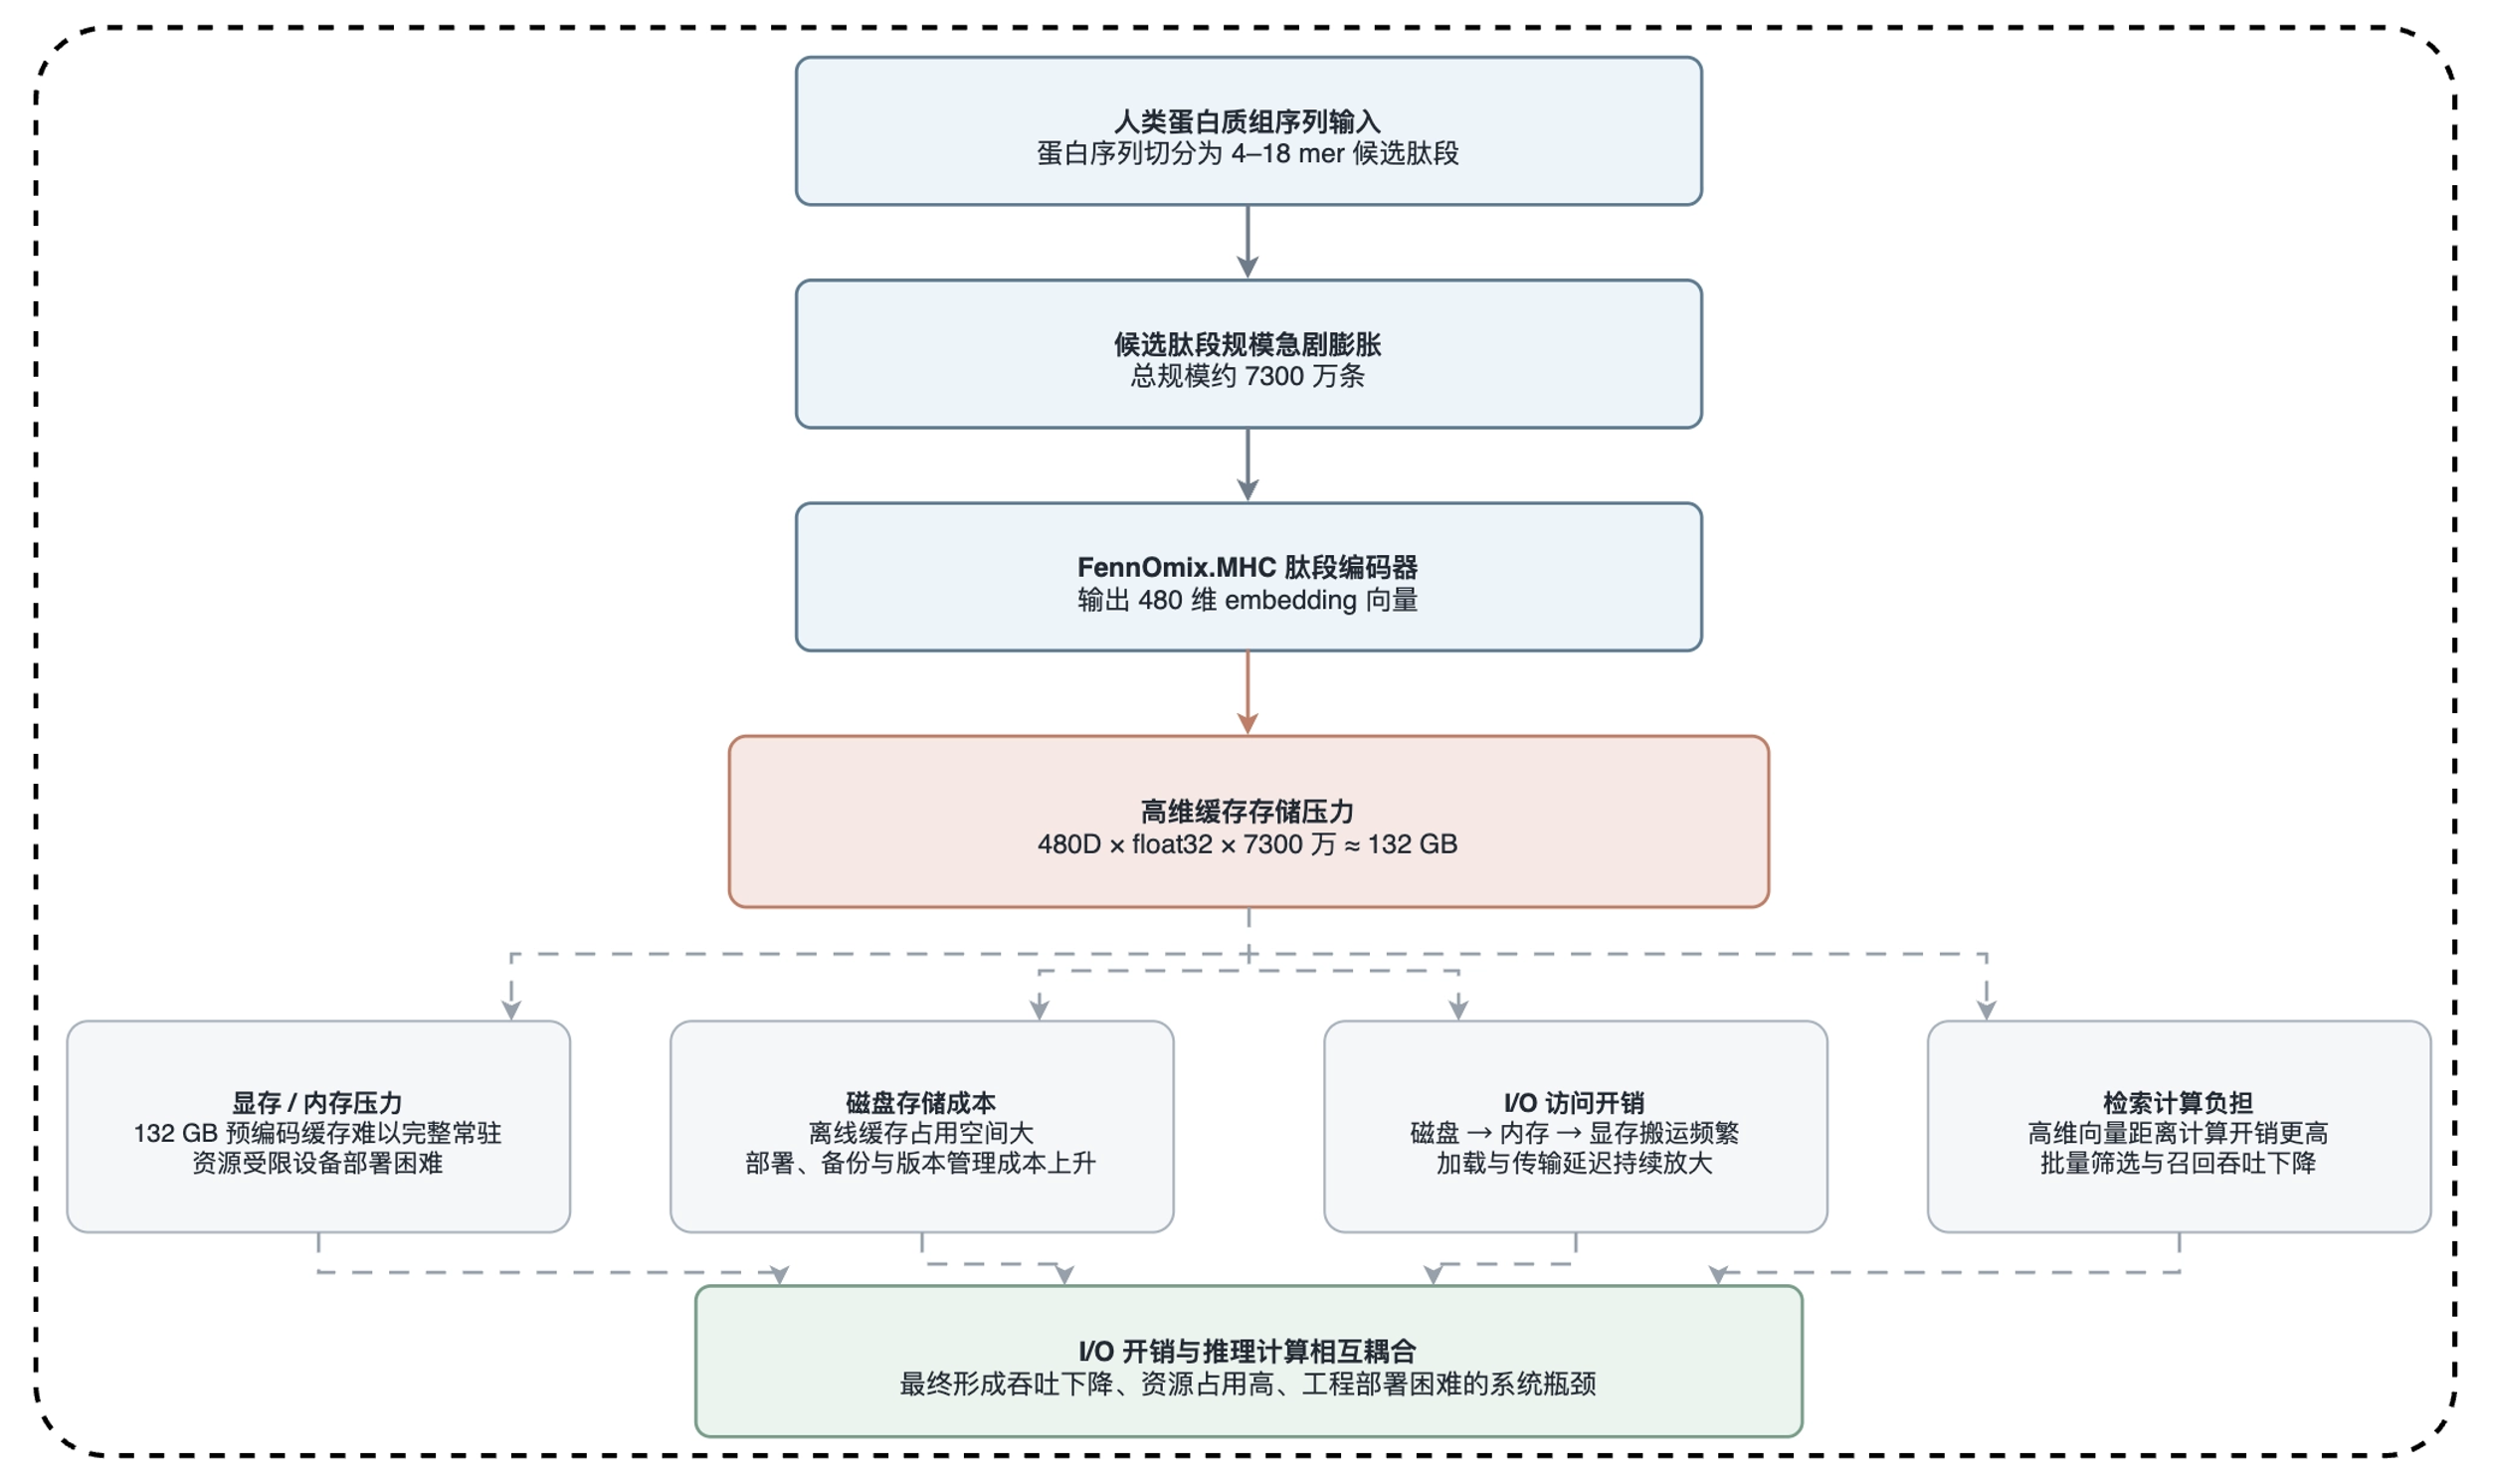
\includegraphics[width=1.0\textwidth]{figures/fig4_bottleneck.png}
    \caption{原始模型部署瓶颈示意图}
    \label{fig:original-model-bottleneck}
\end{figure}

在大规模人类蛋白质组应用中，蛋白质序列会被切割成海量候选肽段，每条肽段均需生成向量表示。如果仍沿用原始的 float32 高维向量进行离线缓存，缓存文件将占用大量存储空间，很难整体驻留在单块 GPU 显存或普通主机内存中，同时还会加重磁盘开销、文件传输、版本管理与部署备份等成本。从工程角度看，肽段缓存过大不仅意味着静态存储成本居高不下，还会拖慢后续模型调用中的读取、加载和数据搬运效率。特别是当候选肽段需要频繁参与距离计算时，缓存规模直接制约着系统响应速度和部署便捷性。因此，压缩肽段 embedding 维度是缓解大规模缓存压力的核心切入点。

原始模型的部署压力并非单纯来自参数量，而是高维向量表示、缓存机制和检索流程相互耦合的结果。维度越高，单次距离计算和批量检索的计算开销越大；缓存越大，数据从磁盘到内存、从内存到显存的搬运成本也越高。系统需要在大规模候选肽段中执行批量筛选时，I/O 延迟与向量计算相互叠加，最终拉低整体吞吐效率。

此外，模型结构本身也可能存在冗余。对于采用 Transformer 结构的编码器，不同注意力头、前馈网络隐藏单元以及不同层模块对最终表示的贡献并不均匀。若不加区分地全部保留，会引入不必要的计算消耗。因此，部署优化不能只盯着输出向量维度，还必须分析模型内部是否存在可压缩的空间。

针对上述瓶颈，我们将 FennOmix.MHC 的模型轻量化优化划分为两个方向：表示压缩与结构压缩。

表示压缩主要回应大规模肽段缓存的压力。通过缩减模型输出 embedding 维度，可以直接降低肽段向量的离线存储开销，并减少后续距离计算和检索过程的时间、空间消耗。对于规模庞大的候选肽段库而言，表示压缩是提升系统可部署性的基础。结构压缩则回应模型推理阶段的冗余计算问题。通过分析 Transformer 编码器中不同注意力头和前馈网络单元的重要性，可以识别贡献较低的组件，进而评估剪枝的可行性。两种压缩并非替代关系，而是互为补充：表示压缩侧重削减输出表示及缓存带来的系统成本，结构压缩则压缩模型内部的计算开销。

基于这一思路，本章将依次介绍编码维度压缩设计、线性和非线性降维方案的构建，以及基于重要性分析的结构剪枝方法。这些方法的具体实验效果将在第三章进行验证。

\subsection{编码维度压缩设计}

编码降维是本文面向部署优化的第一步，其核心并非单纯压缩向量维度，而是在守住 MHC-I 肽段结合预测能力和嵌入空间结构稳定性的前提下，显著削减肽段预编码缓存的存储成本。FennOmix.MHC 后续的大规模候选筛选、距离排序以及下游缩库辅助搜库，都依赖于 embedding 空间的几何关系。因此，一个合理的降维方案需同时满足以下三点：第一，候选排序能力保持基本稳定，降维后的模型仍能将真实结合肽段排在候选列表前部；第二，嵌入空间的邻域结构尽量得到保留，真实结合肽段仍聚集在对应 HLA 表示附近；第三，缓存体积明显下降，体现出工程价值。

这实际上是将输出维度压缩定位为“预测性能—空间结构—存储成本”三者的权衡，而不是一味追求最低维度。为考察不同输出维度对模型性能和缓存成本的影响，我们设置了多组输出维度方案，包括原始高维表示和若干低维压缩表示，以此观察维度逐步降低时，性能、结构稳定性和缓存成本之间的变化关系。

评价方面，我们联合使用两类指标：基于排名阈值的 rank-recall，评估模型在大规模候选筛选中的排序能力；基于欧氏距离阈值的 distance-recall，评估真实结合样本在共享嵌入空间中的邻域聚集程度。它们分别对应“候选排序能力”和“空间结构保持性”，可以从不同侧面反映降维带来的影响。缓存成本则通过 $S = N \times D \times B$ （其中， $N$ 是候选肽段数量，$D$ 是向量维度，$B$ 是每个元素占用字节）估算，在候选肽段数量和数据类型固定的条件下，缓存规模与输出维度近似线性相关，降低维度能直接缩减缓存体积。

在输出维度的选取上，最低维度并不是唯一目标。维度过高，缓存和计算成本依然偏高；维度过低，则可能破坏嵌入空间结构，损害候选排序和后续检索效果。因此，合理的维度应在性能保持与成本降低之间找到平衡。我们主要依据以下原则来选择后续重点优化的方案：优先确保嵌入空间结构稳定，distance-recall 是判断降维可接受的重要依据；兼顾候选排序能力，尽可能维持较好的 rank-recall；关注缓存压缩带来的实际收益，若某维度方案在性能下降可控的同时显著缩减缓存，则更适合作为后续缓存压缩、索引检索和系统部署的基础。第三章将对不同维度方案进行系统的实验比较，并据此确定适用于后续部署优化的默认输出维度。

\subsection{线性与非线性降维方案设计}

在输出维度压缩的基础上，还需比较相同维度条件下不同映射结构对模型性能和部署成本的影响。为此，我们设计了线性降维和非线性降维两类方案：线性降维采用单层线性映射，将上游编码结果直接投影到目标低维空间；非线性降维采用包含隐藏层和激活函数的 MLP 结构。线性方案结构简单、参数量少，易于训练和部署；MLP 表达力更强，但会引入额外的参数和计算开销。

实验中构建了两个 64 维低维模型进行对照：MHC-64D-BertLinear 和 MHC-64D-BertMLP，在输出维度一致的条件下比较，保证差异主要来源于映射结构本身。

首先采用常规的 rank-recall 和 distance-recall 评估两类模型的基础预测能力。若两者在常规指标上表现接近，单靠这些指标不足以做出取舍，还需要结合下游任务和模型复杂度进一步判断。为此，我们进一步引入缩库辅助数据库检索任务。模型先根据目标 HLA 对候选肽段进行筛选，构建等位基因特异的缩减数据库，再将这一缩库结果与直接检索流程进行肽段重叠比较。评价采用 Precision-like、Recall-like、Overlap-F1、Loss Rate、Expansion Rate 和 Comprehensive Score 等指标，从覆盖度、一致性、结果丢失和新增差异等角度衡量缩库效果。将 Linear 和 MLP 两类模型嵌入相同的下游流程进行比较，能更真实地反映不同降维结构在实际应用场景中的适用程度。

最终默认降维模型的选定需要综合三方面因素：常规预测性能应在 rank-recall 和 distance-recall 上保持相对稳定，表明候选排序和空间结构未受明显冲击；下游缩库辅助搜库任务中应保持较好的覆盖度和一致性，体现其在实际流程中的价值；同时优先选择工程部署成本更低的方案。若 Linear 与 MLP 的性能差别不大，则结构更轻量、参数更少、实现更简单的 Linear 更适合作为默认部署模型。第三章将结合常规指标与下游缩库辅助搜库结果，对两类降维模型进行全面比较，并确定后续系统优化所采用的默认模型。

\begin{figure}[htbp]
    \centering
    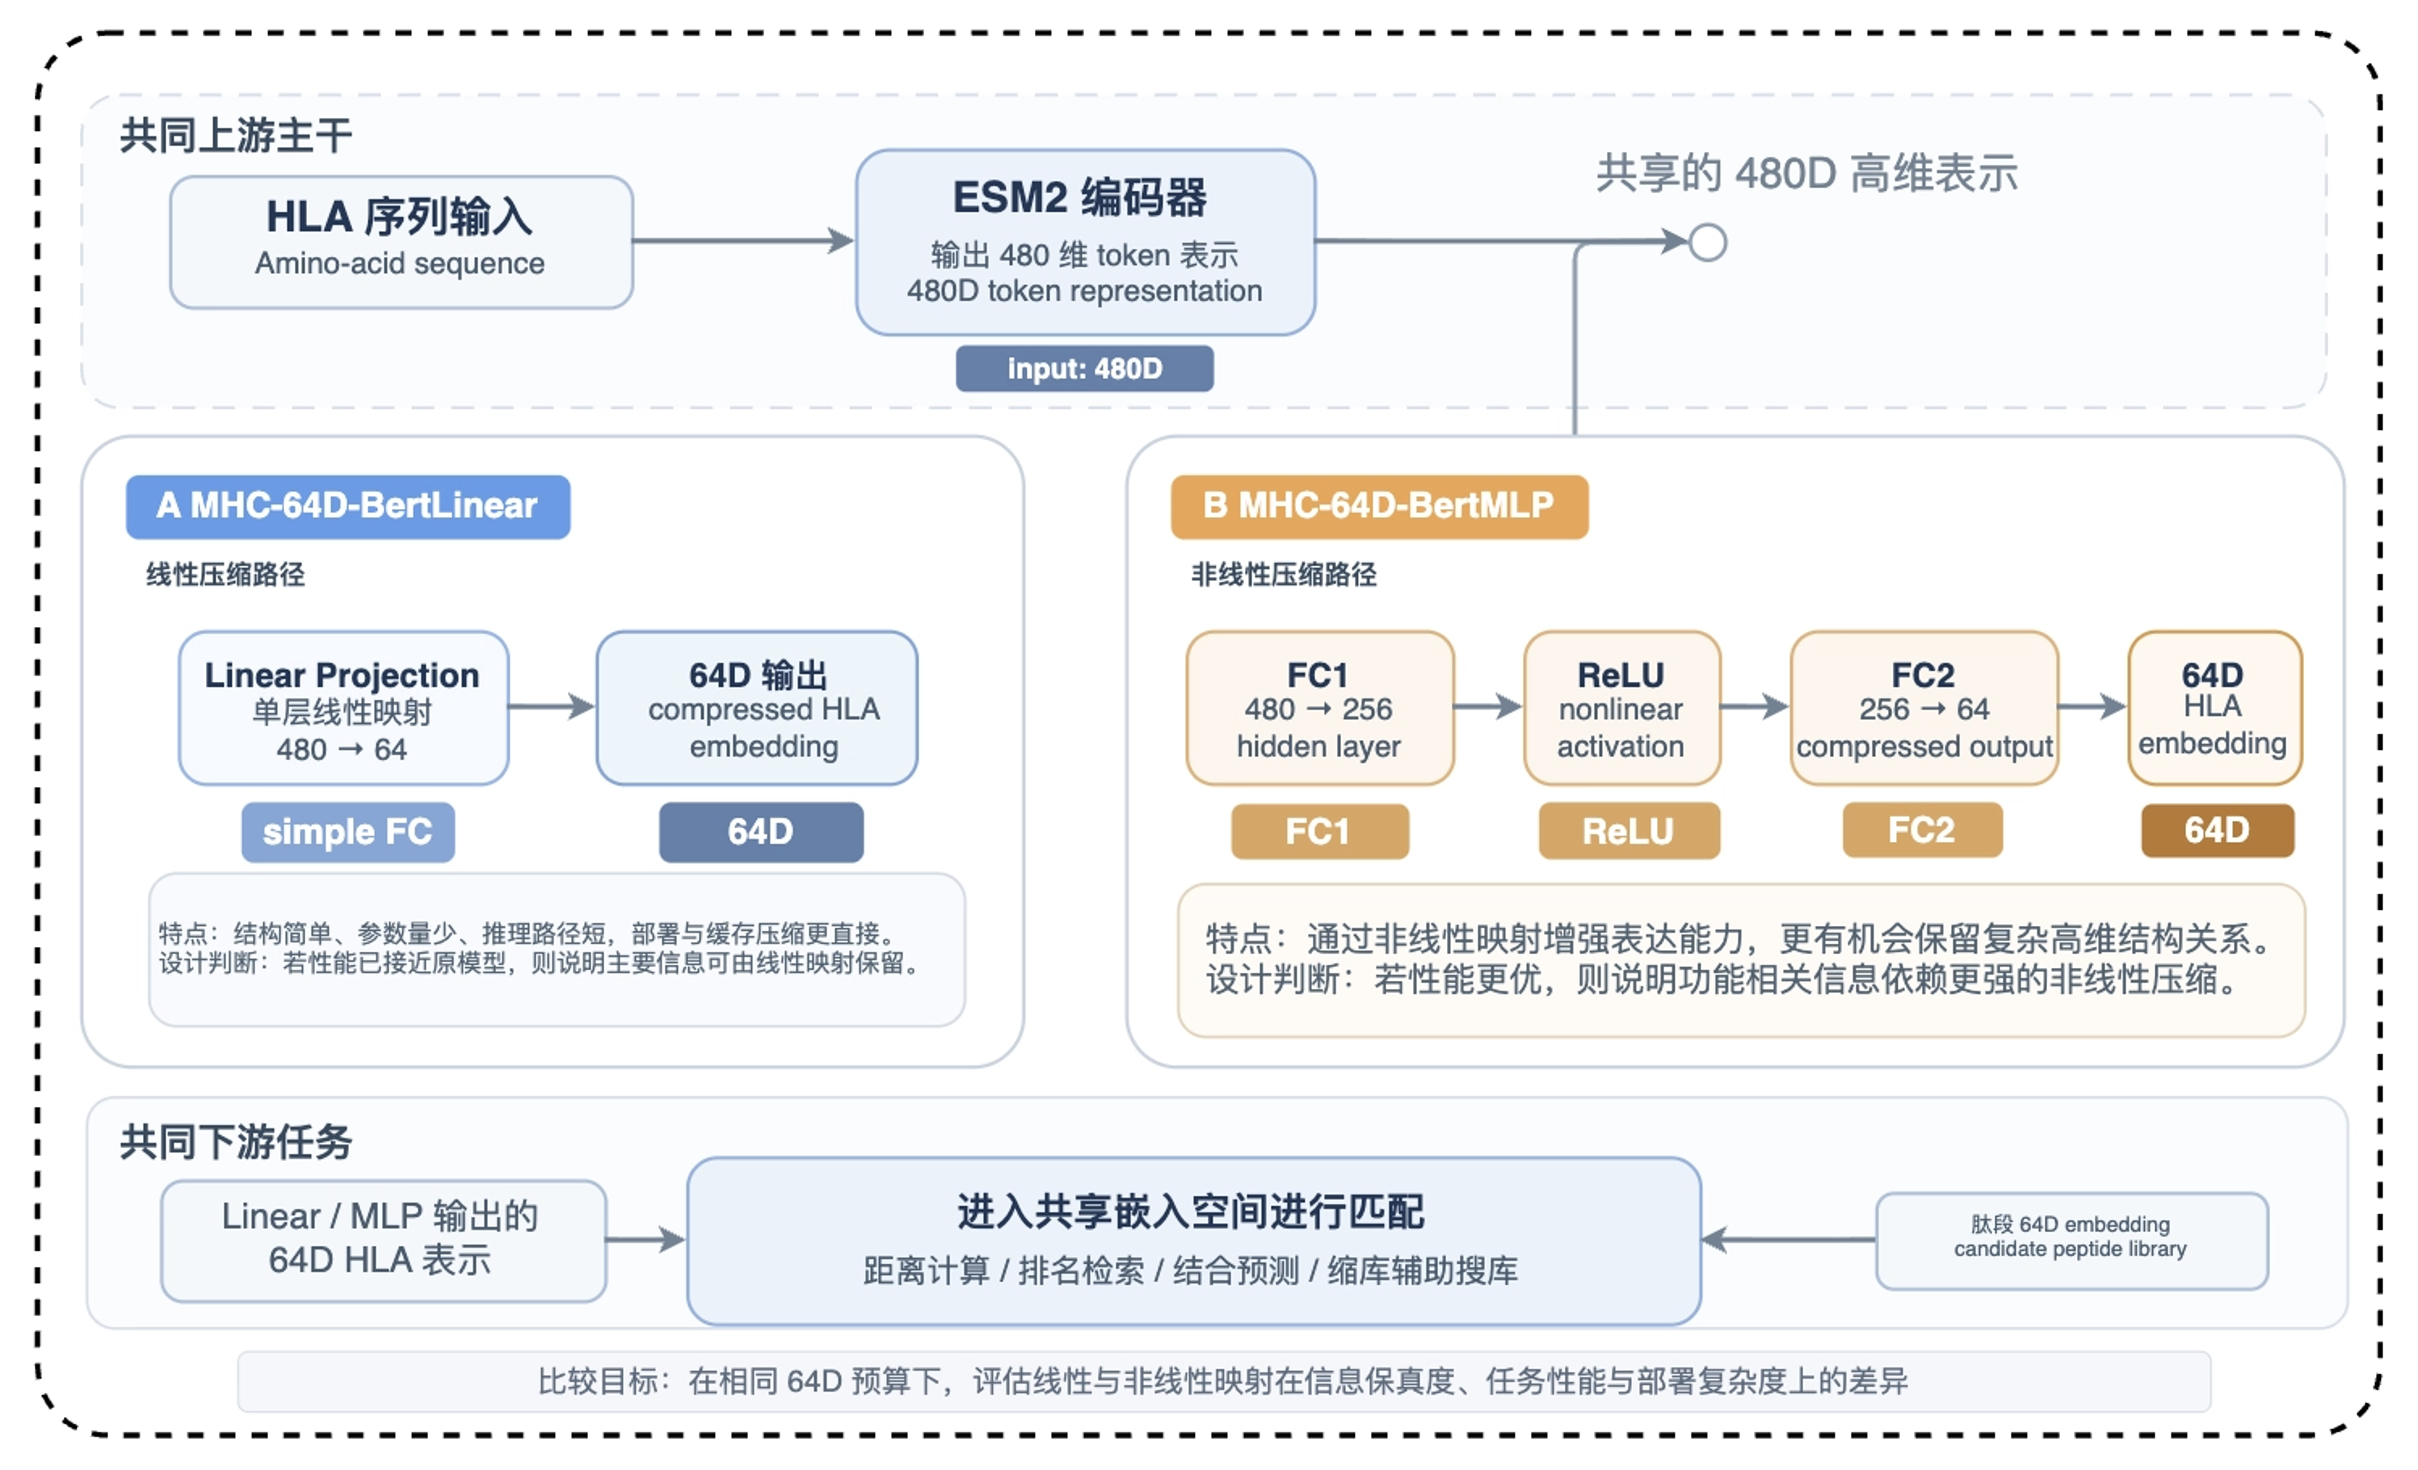
\includegraphics[width=1.0\textwidth]{figures/fig5_linear_mlp.png}
    \caption{Linear 与 MLP 的结构对比图}
    \label{fig:linear-mlp-structure}
\end{figure}

在该任务中，模型先根据目标 HLA 对候选肽段进行筛选，构建等位基因特异的缩减数据库；随后将这一缩库结果与直接检索流程进行比较。通过分析两种流程在肽段层面的 overlap，可以评价模型辅助缩库在压缩候选空间的同时能否有效保留基线检索结果。

本文采用 Precision-like、Recall-like、Overlap-F1、Loss Rate、Expansion Rate 和 Comprehensive Score 等指标，从覆盖度、一致性、结果丢失及新增差异等角度评价缩库效果。将 Linear 与 MLP 两类模型嵌入相同的下游流程进行比较，能够进一步判断不同降维结构在真实应用场景中的适用程度。

最终默认降维模型的选定需要综合多重因素，而不能仅依赖单一指标。本文主要从以下三个方面加以判断。

第一，常规预测性能。模型应在 rank-recall 和 distance-recall 上保持相对稳定，说明其候选排序能力和空间结构保持能力未受到明显冲击。第二，下游任务表现。模型应在缩库辅助搜库任务中保持较好的结果覆盖度和一致性，表明其不仅在测试指标上有效，也能在实际应用流程中发挥作用。第三，工程部署成本。若两类模型的性能差别不大，则结构更轻量、参数更少、实现成本更低的方案更适合作为默认部署模型。

因此，本文将于第三章结合常规预测指标与下游缩库辅助搜库结果，对 Linear 与 MLP 两类降维模型进行全面比较，并确定后续系统优化所采用的默认模型。

\subsection{基于重要性分析的结构剪枝}

在表示降维之后，我们从模型结构层面继续探索轻量化的空间。与输出降维主要降低缓存和距离计算成本不同，结构剪枝直接作用于模型内部网络，旨在削减编码器推理时的冗余计算。

FennOmix.MHC 的编码器采用了 Transformer 结构，其中的注意力头和前馈网络单元对最终表示的贡献并不均等，因此我们将剪枝目标聚焦于 attention head 和 Feed-forward Network（FFN）隐藏单元，通过分析它们的贡献来识别冗余部分。

我们的剪枝思路是：在训练或评估阶段收集各组件激活或梯度的信息，据此计算重要性指标并排序，随后移除低重要性组件，再通过实验检验剪枝后的性能保持情况。

为了判断哪些组件可以安全移除，需要为注意力头和前馈网络单元建立可比较的重要性指标。我们采用基于激活和梯度的分析方法，来衡量不同组件对模型输出的贡献。

对于注意力头，可以统计其输出激活的范数或与损失相关的梯度范数；如果在多个批次中某个注意力头持续表现出较低的激活或梯度，则意味着它的贡献可能较弱。前馈网络隐藏单元也可通过类似的激活强度或梯度响应来估计重要性。

不同层的数值尺度可能不同，因此需要对重要性分数进行归一化。我们可以在层内或全模型范围内进行组件得分比较，以避免单层数值整体偏高或偏低带来的干扰。得分较高的组件视为关键结构予以保留，得分较低且稳定的则作为候选剪枝对象。

这样，剪枝就不再是盲目的结构删除，而是依据贡献差异进行选择性压缩，有助于降低性能损失的风险。

在具体实现上，我们采用基于重要性排序的结构压缩。首先，用验证集或测试集对模型进行前向传播和必要的梯度计算，收集注意力头和前馈网络单元的激活或梯度信息；然后，对重要性分数进行累积和归一化，得到综合排序结果。

对于注意力头，根据重要性分数选出低贡献的 head，可以通过置零权重、屏蔽输出或结构性移除等方式来降低其影响。对于前馈网络单元，则按隐藏单元的重要性分数确定剪枝位置，移除低贡献单元或缩减中间层维度。

剪枝后，需要验证模型性能是否明显下降。我们从预测能力和部署收益两个维度来评价剪枝效果。

预测能力方面，剪枝后的模型仍需通过 rank-recall 和 distance-recall 等指标来测试，以判断候选排序能力和嵌入空间结构是否受损。如果表现保持稳定，则说明被移除的组件大概率是冗余的。

部署收益方面，关注剪枝对参数规模、计算量和推理效率的影响。结构化剪枝若能真正减少矩阵计算规模，就有可能降低推理延迟和资源占用；掩码式剪枝可以论证冗余的存在，但实际加速效果还需要结合具体实现来评估。

因此，剪枝实验不仅是为了观察性能变化，更在于验证模型内部存在可压缩的冗余，为后续更细粒度的结构优化提供依据。具体的剪枝结果和性能对比将在第三章给出。

\begin{figure}[htbp]
    \centering
    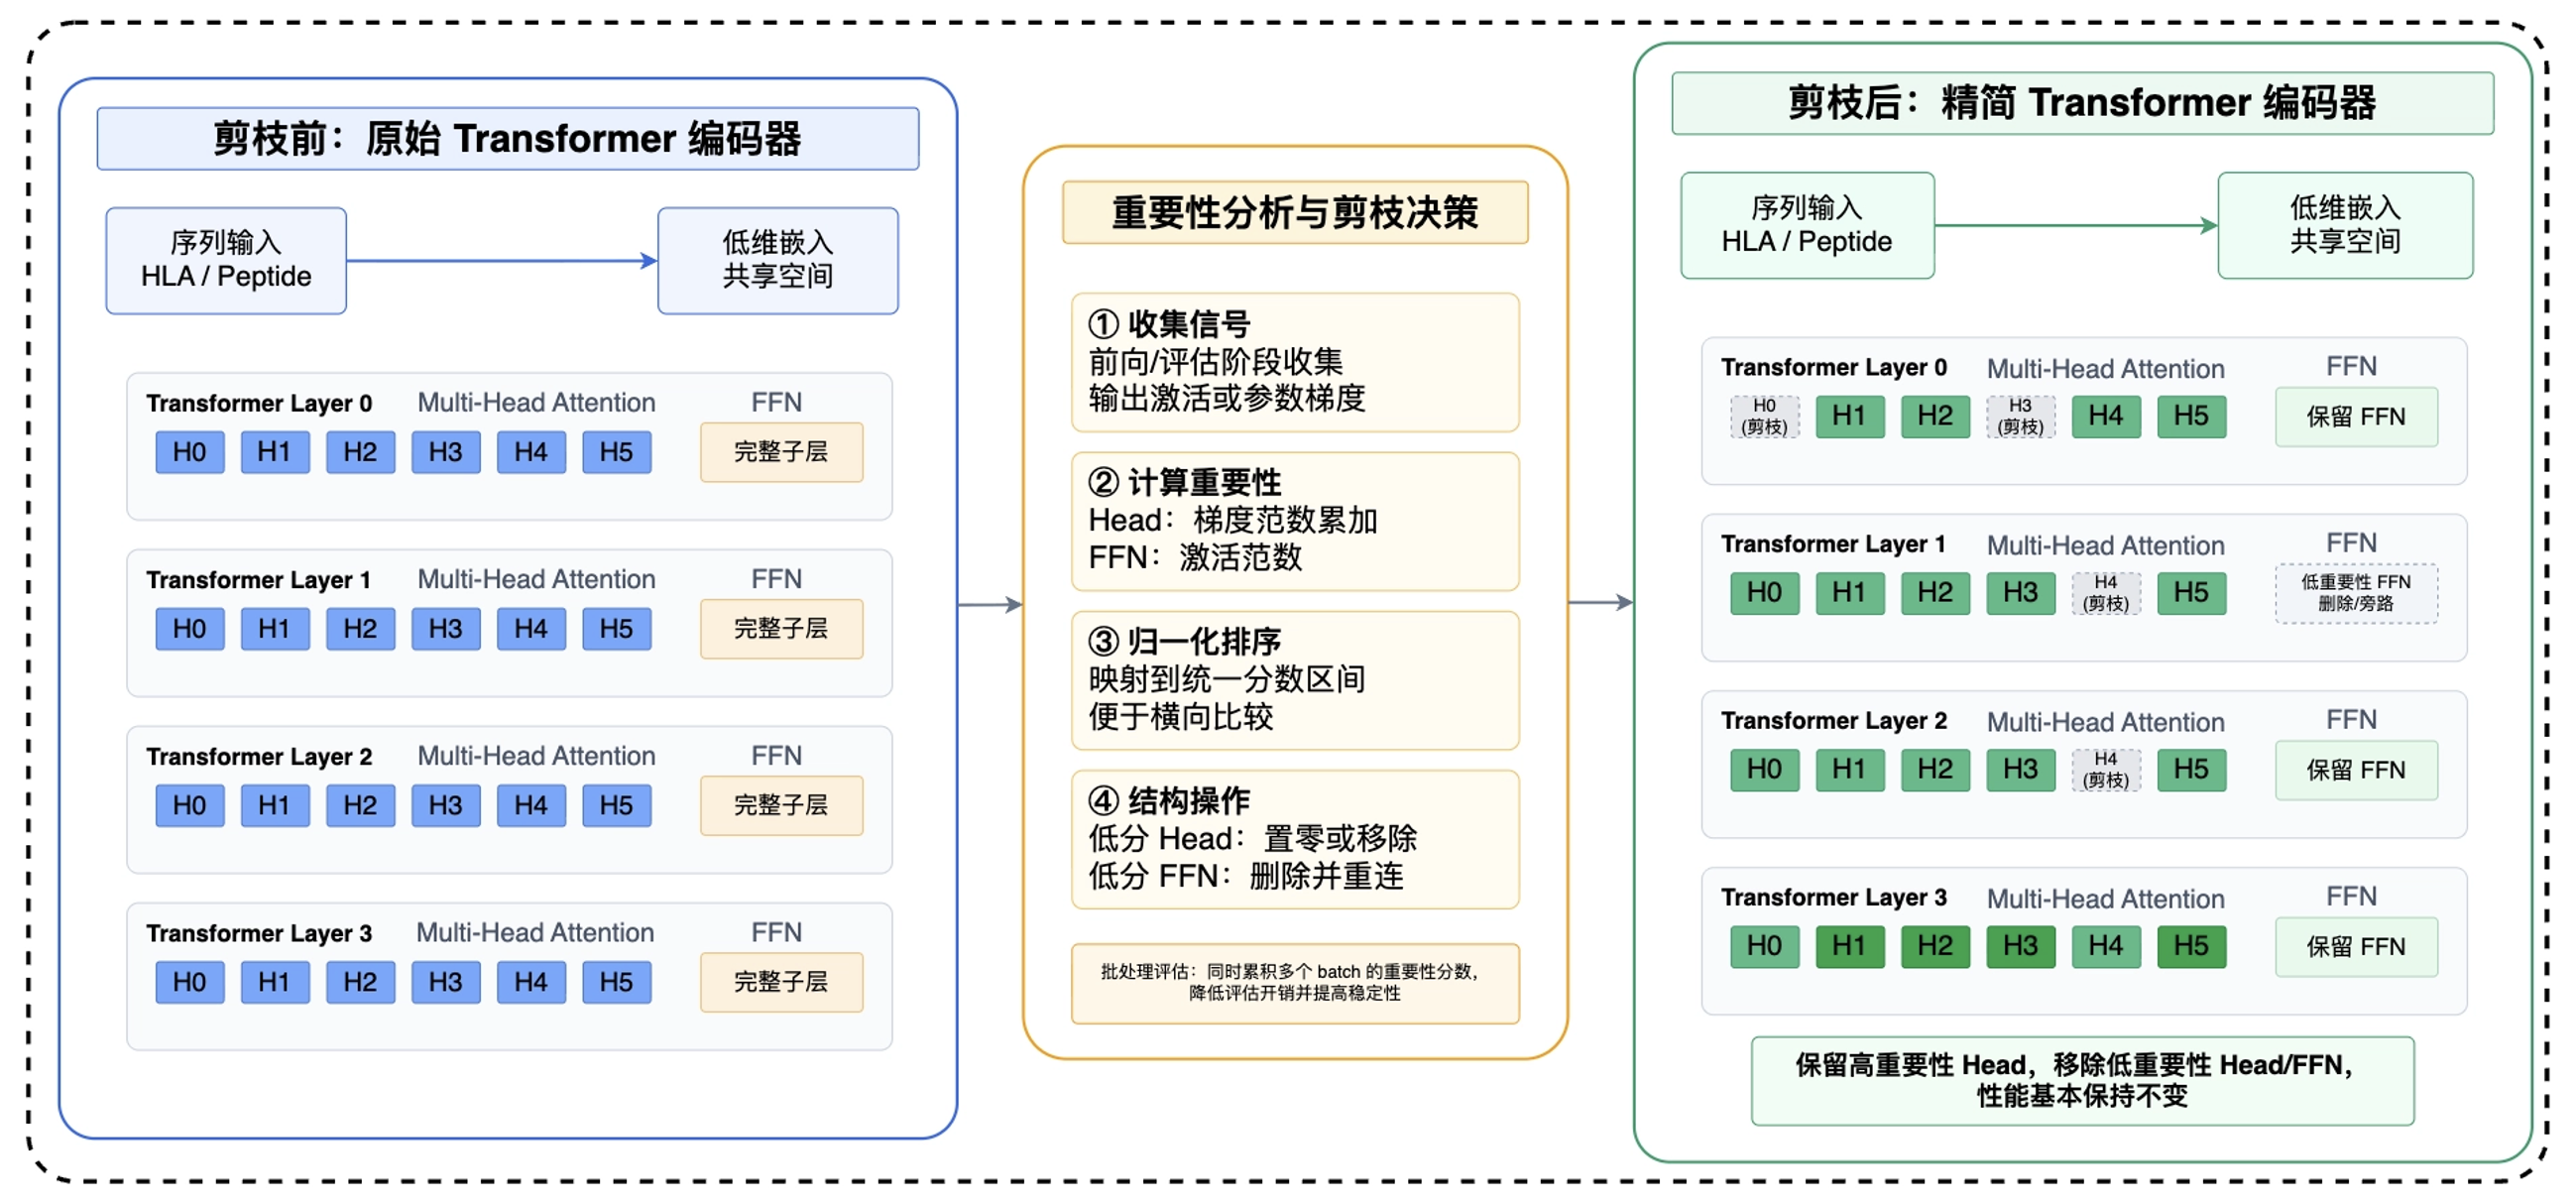
\includegraphics[width=1.0\textwidth]{figures/fig6_pruning_structure.png}
    \caption{剪枝前后结构示意图}
    \label{fig:pruning-structure}
\end{figure}

\section{肽段缓存压缩与索引机制设计}

\subsection{大规模肽段缓存问题}

在大规模候选肽段筛选与检索中，如果每次查询都实时调用肽段编码器重新生成 embedding，计算开销会非常大，系统响应速度也会明显下降。因此，预先对常见肽段进行批量编码并离线缓存，是支撑快速检索的关键前提。

借助缓存，在线阶段可以直接复用已有的肽段向量，只需对目标 HLA 或少量缓存外肽段实时编码，从而大幅减少重复推理。对于候选肽段规模庞大的场景，离线预计算与在线复用相结合，是提升可部署性和查询效率的重要方式。

然而，缓存在加速的同时也带来了新的系统问题。在大规模人类蛋白质组场景中，即便已经通过模型降维压缩了肽段 embedding 的维度，如果仍以 float32 精度存储，缓存体积依然偏大，会继续加重磁盘占用、内存加载和数据读取的负担。因此，在输出维度压缩后，仍有必要对缓存的表示方式和访问组织做进一步优化。

从系统设计看，肽段缓存主要面临两对矛盾。

第一，存储成本与表示精度相互制约。更高精度的浮点表示能更完整地保留模型输出，但存储体积也随之膨胀。若将所有肽段 embedding 以 float32 原样存储，缓存文件不仅占空间，也不利于跨环境传输、版本管理和长期归档。因此，需要在确保向量近似精度的前提下，引入更紧凑的数据表示。

第二，访问效率与资源占用彼此掣肘。将缓存向量一次性全部加载到内存，查询速度快，但内存压力也大；始终保留在磁盘中按需读取，虽然减轻了常驻内存负担，但在高频查询时容易受到 I/O 延迟的影响。这就需要系统根据不同场景设计灵活的加载策略，在访问效率和资源消耗之间找到平衡。

基于上述问题，我们从两个层面设计缓存机制：一方面，对低维肽段向量进一步采用 INT8 量化压缩来缩减缓存文件体积；另一方面，围绕缓存文件建立肽段索引，并设计全量加载和延迟加载两种访问模式，以适配不同的查询频率和资源条件。

\subsection{基于INT8的缓存量化压缩}

肽段缓存压缩的核心诉求并不是一味追求最小体积，而是在尽可能保持 embedding 表示精度的前提下，减少缓存的存储和传输开销。后续肽段向量还要与目标 HLA 嵌入进行距离计算，过大的压缩误差可能影响候选筛选的可靠性。因此，缓存压缩方法需要在压缩率、数值误差和实现复杂度之间取得平衡。

我们采用基于线性量化的对称 INT8 压缩方案，将原始 float32 向量映射为 INT8 表示。该方法的优点是压缩与反压缩计算简单，适合大规模批量处理；逐维缩放因子保留了各维度的数值尺度信息，有助于减小因维度分布差异带来的误差。

记肽段编码器输出的原始向量矩阵为 $X \in \mathbb{R}^{N \times D}$ ，其中，$N$ 为肽段总数，$D$ 为 embedding 维度，$x_{ij}$ 表示第 $i$ 条肽段在第 $j$ 维上的浮点值。

对每个维度 $j$，首先统计其均值和标准差：
\[
    \mu_j
    =
    \frac{1}{N}
    \sum_{i=1}^{N} x_{ij},
\]

\[
    \sigma_j
    =
    \sqrt{
        \frac{1}{N}
        \sum_{i=1}^{N}
        \left(x_{ij}-\mu_j\right)^2
    }
\]
为减轻极端值对量化范围的影响，本文采用基于 $k\sigma$ 的截断策略确定各维度的对称量化范围。令： $a_j = k\sigma_j$ ，由此，第 $j$ 维的量化区间为： $\left[-a_j, a_j\right]$ ，在此基础上，第 $j$ 维的缩放因子、截断值和量化整数可统一表示为： $s_j = \frac{a_j}{127}$ ，其中，127 对应 INT8 有符号整数正向范围的最大值。

为避免溢出，量化前先对原始浮点值进行截断：
\[
    \hat{x}_{ij}
    =
    \mathrm{clip}
    \left(
        x_{ij},
        -a_j,
        a_j
    \right)
\]
随后，利用缩放因子将浮点值映射为整数：
\[
    q_{ij}
    =
    \mathrm{round}
    \left(
        \frac{\hat{x}_{ij}}{s_j}
    \right)
\]
其中： $q_{ij} \in \left[-127,127\right]$ 。

量化后的 $q_{ij}$ 以 INT8 类型保存。对整个肽段向量矩阵而言，量化后的整数矩阵可表示为： $Q \in \mathbb{Z}^{N \times D}$ 。

在实际使用时，系统读取量化后的整数值 $q_{ij}$ 及对应维度的缩放因子 $s_j$，通过反量化即可恢复浮点近似值： $\widetilde{x}_{ij} = q_{ij} \cdot s_j$ 。

于是，原始 float32 向量便可表示为“INT8 数据块 + 逐维缩放因子”的组合，前者承载压缩后的主体数据，后者用于复原数值尺度。

量化误差可表示为原始浮点值与反量化近似值之差： $e_{ij} = x_{ij} - \widetilde{x}_{ij}$ 。

在不计截断误差的理想情形下，线性量化将连续区间划分为固定步长的离散取值，由四舍五入引起的单元素误差上界近似满足： $\left|e_{ij}\right| \le \frac{s_j}{2}$ 。

由上式可知，量化误差主要受缩放因子 $s_j$ 控制。缩放因子越小，离散化步长越细，量化误差越低；缩放因子越大，量化范围虽宽，但单个取值间隔也相应增大。因此，在设定量化范围时，应避免极端值过度拉大 $a_j$，否则会损害大部分样本的量化精度。

本文采用逐维独立量化，而非对所有维度使用统一缩放因子，原因在于不同 embedding 维度的数值分布可能存在差异，逐维缩放能更好地适配各维度的尺度变化，从而压低量化误差。后续第三章将通过实验统计量化前后的误差，并分析该压缩方法对缓存存储和向量表示的影响。

从存储角度看，float32 数据每个元素占 4 字节，INT8 每个元素占 1 字节。因此，在忽略少量缩放因子与文件头开销的情况下，向量主体数据体积可近似压缩至原来的四分之一，这为大规模肽段缓存的落盘、加载和传输提供了更紧凑的数据基础。

\subsection{自定义二进制缓存格式}

仅靠量化方法尚不足以构成完整的缓存机制，还需配合一种适宜批量存储与按索引访问的数据组织格式。若继续采纳文本格式或逐条对象序列化方式保存向量，不但会引入显著的额外开销，也不利于后续的随机访问和高效读取。有鉴于此，本文在量化之后进一步设计了自定义二进制缓存格式，用以组织大规模肽段向量数据。

与通用序列化方式相比，自定义二进制格式更契合本文的数据特征：向量维度固定、肽段数量庞大，且查询模式以按索引定位为主。针对这种“定长向量 + 大规模顺序块”的结构，紧凑的二进制布局能有效削减冗余元数据，并提升基于偏移量的读取效率。

本文设计的自定义二进制缓存文件主要由文件头、缩放因子区、量化数据区和肽段序列区构成，各部分功能如表~\ref{tab:binary-cache-format} 所示。

文件头赋予缓存文件自描述能力：系统读取文件头即可校验格式、版本，并获取肽段数量与向量维度等元信息。缩放因子区存放各维度对应的浮点缩放因子，供反量化时还原近似浮点向量。向量数据区以连续块形式保存所有肽段的 INT8 向量，使得系统能够按索引位置直接计算偏移量并读取对应的压缩数据。肽段序列区则记录各向量对应的原始肽段字符串，为后续哈希索引的构建提供基础。

自定义二进制格式并非孤立设计，而是与后续索引机制紧密衔接。由于所有量化向量按固定维度顺序连续存放，一旦获知某肽段对应的索引编号，即可直接计算出其在量化数据区中的偏移量。

设每个量化向量的维度为 $D$，每个 INT8 元素占 1 字节，第 $i$ 个肽段向量在数据区中的起始偏移量为：
\[
    \mathrm{offset}_i
    =
    \mathrm{offset}_{\mathrm{data}}
    +
    i \times D
\]
其中，$\mathrm{offset}_{\mathrm{data}}$ 为量化数据区的起始位置。通过该偏移量，系统可直接定位并读取第 $i$ 个肽段的压缩向量。

\begin{table}[htbp]
    \centering
    \caption{自定义二进制缓存文件结构}
    \label{tab:binary-cache-format}
    \begin{tabular}{p{0.18\textwidth} p{0.36\textwidth} p{0.36\textwidth}}
        \toprule
        区域 & 内容 & 作用 \\
        \midrule
        文件头
        & magic、version、肽段数量 $N$、向量维度 $D$、数据类型等
        & 标识文件格式，记录基础元数据 \\

        缩放因子区
        & 每个维度对应的缩放因子 $s_j$
        & 用于 INT8 向量反量化 \\

        向量数据区
        & 连续存储的 INT8 向量块
        & 保存压缩后的肽段 embedding \\

        肽段序列区
        & 肽段字符串列表或偏移表
        & 支持索引构建和查询定位 \\
        \bottomrule
    \end{tabular}
\end{table}

由此可见，二进制缓存格式为“按索引随机访问向量”提供了底层数据支撑，而索引模块则负责完成从“肽段字符串”到“向量位置”的映射。两者协同后，系统便能在在线查询阶段迅速判断缓存是否命中并读取对应向量。

\subsection{肽段哈希索引与加载策略}

完成缓存压缩后，系统还需应对另一关键问题：面对任意输入肽段，如何快速判断其是否已存于缓存，并在命中时即刻定位相应的嵌入向量。

为此，本文设计了基于“预计算缓存 + 字典查找”的肽段索引策略。其核心思路是将大规模候选肽段的编码工作前移至离线阶段，在线阶段则借助索引结构快速定位缓存向量。这样一来，系统在线阶段的主要任务便从“重复编码 + 遍历搜索”转化为“索引定位 + 向量读取”，从而有效缩短响应时间。

该策略尤其适合候选库规模庞大的场景。若在在线查询时逐条比对或重新编码，将很难满足响应需求。通过预计算缓存与索引查找，可以充分复用离线计算结果，显著提升常见肽段的查询效率。

索引结构定义为一个字典映射：
\[
    \mathrm{peptide\_index}
    :
    \mathrm{Dict}
    \left[
        \mathrm{str},
        \mathrm{int}
    \right]
\]
其中，索引以肽段序列字符串为键，对应的值是该肽段向量在缓存文件中的位置编号。在线查询时，系统会在 peptide\_index 中查找输入肽段：命中则直接返回位置编号，未命中则转入实时编码流程。

这种设计的查询效率很高。哈希字典的平均键值查找复杂度接近 $O(1)$，无需遍历全部候选肽段就能快速完成序列到缓存位置的定位。

从实现角度，索引必须与缓存文件严格保持同步。一旦缓存文件重新生成、肽段顺序调整或模型版本变更，索引也需要随之更新，否则可能出现位置与向量数据错位，影响查询准确性。

\begin{figure}[htbp]
    \centering
    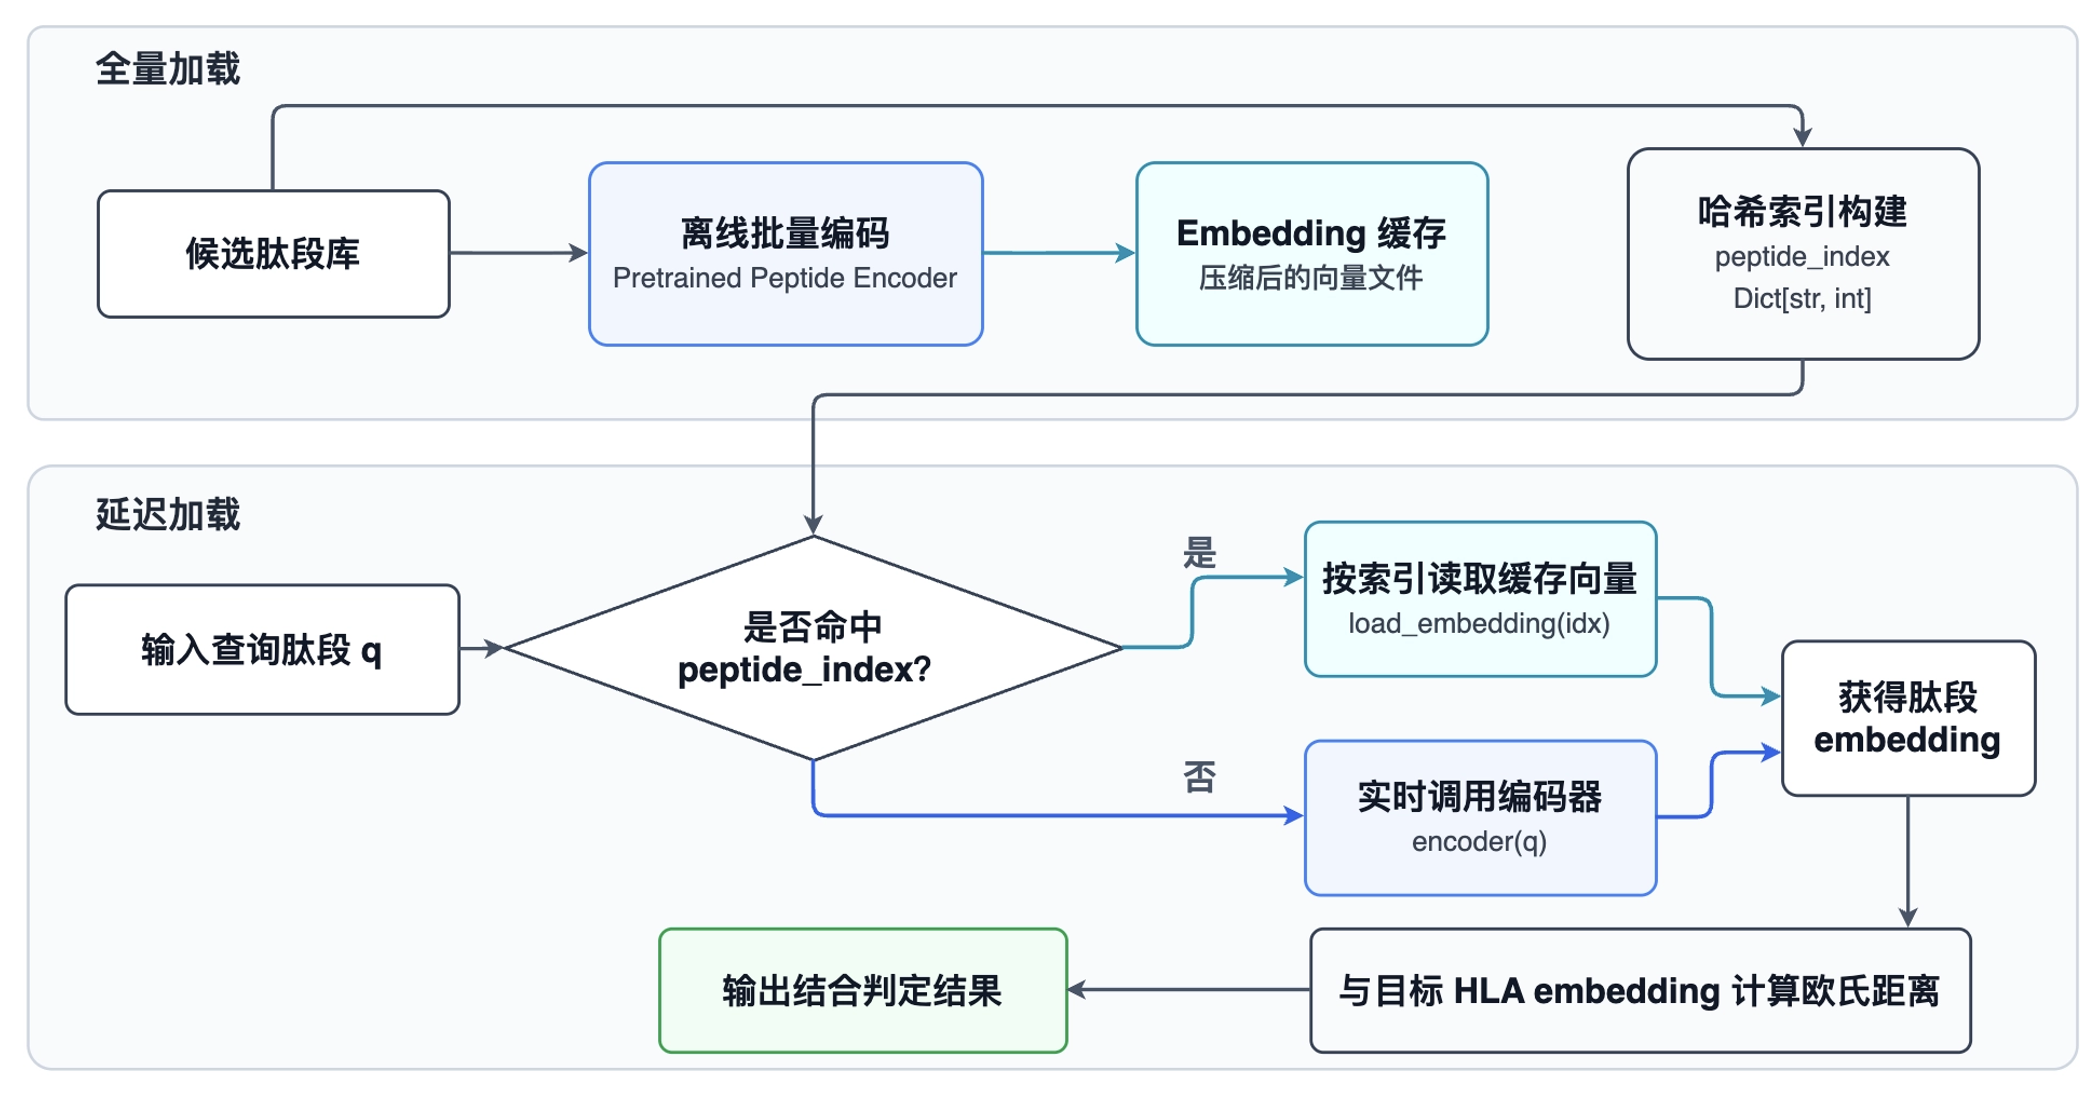
\includegraphics[width=1.0\textwidth]{figures/loading_strategy.png}
    \caption{全量加载与延迟加载结构图}
    \label{fig:loading-strategy}
\end{figure}

为了在访问速度和资源占用之间取得平衡，我们设计了两种加载模式：全量加载和延迟加载。

全量加载模式在系统启动时就把所有缓存向量读入内存。查询命中索引后，可以直接从内存数组中取出向量，访问速度很快，适合高频查询、批量筛选或内存充裕的服务器场景，但会占用较多的常驻内存。

延迟加载模式只在启动时加载肽段列表和索引结构，不立即载入全部向量。当某个肽段命中索引后，再根据其位置从磁盘缓存文件中读取向量。这种方式适合查询量不大或内存紧张的环境，能降低常驻内存压力，但在高频随机访问时容易受磁盘 I/O 制约。两种模式的实际资源收益将在第三章实验分析和第四章部署分析中详细说明。

\subsection{在线查询与匹配执行流程}

\begin{figure}[htbp]
    \centering
    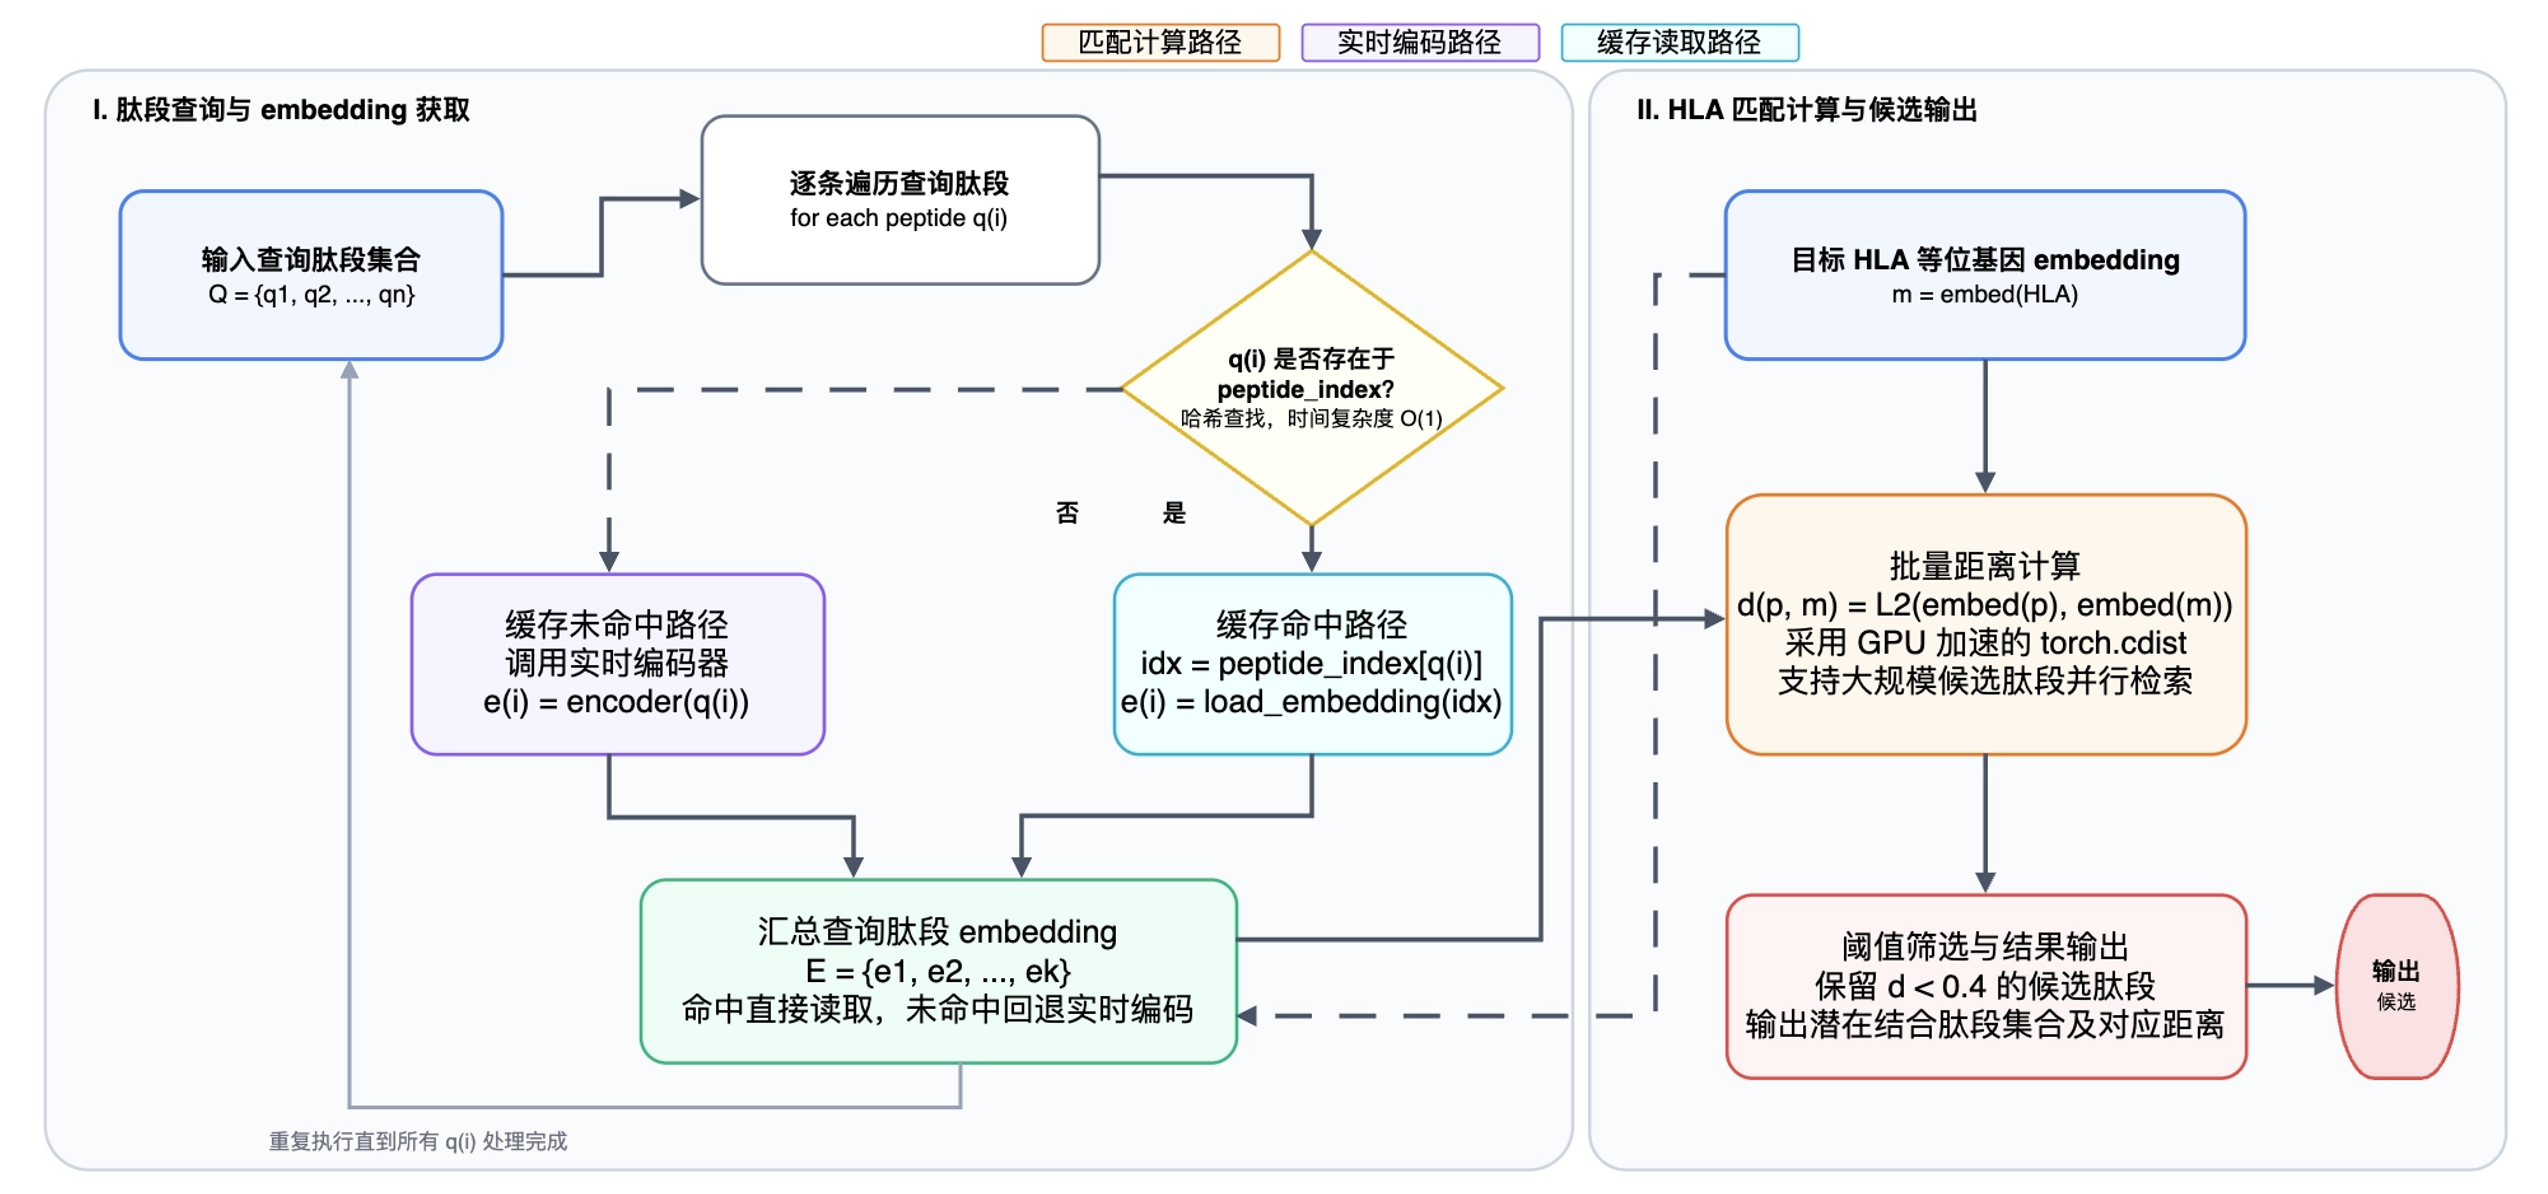
\includegraphics[width=1.0\textwidth]{figures/query_flow.png}
    \caption{完整查询流程图}
    \label{fig:query-flow}
\end{figure}

设输入查询肽段集合为 $Q = \left(q_1, q_2, \ldots, q_n\right)$，输出为对应的 embedding 集合 $E = \left(e_1, e_2, \ldots, e_n\right)$。

对每个查询肽段 $q_i$，系统先判断它是否在 \textit{peptide\_index} 中：如果在，就读取对应的缓存向量；如果不在，则调用肽段编码器实时生成 embedding。这样既复用了缓存，也保留了对新肽段的开放处理能力。

% 查询肽段向量获取流程的伪代码如下：

% \begin{tcolorbox}[
%     breakable,
%     enhanced,
%     colback=white,
%     colframe=black,
%     boxrule=0.5pt,
%     arc=0pt,
%     width=0.90\textwidth,
%     center,
%     left=6pt,
%     right=6pt,
%     top=6pt,
%     bottom=6pt
% ]
%     \ttfamily
%     输入：查询肽段集合 $Q$，肽段索引 peptide\_index，缓存文件 cache，肽段编码器 encoder\\
%     输出：肽段向量集合 $E$\\[0.5em]

%     E = []\\
%     for q in Q:\\
%     \hspace*{2em}if q in peptide\_index:\\
%     \hspace*{4em}idx = peptide\_index[q]\\
%     \hspace*{4em}e = load\_embedding(cache, idx)\\
%     \hspace*{2em}else:\\
%     \hspace*{4em}e = encoder(q)\\
%     \hspace*{2em}E.append(e)\\[0.5em]
%     return E
% \end{tcolorbox}

这一流程的好处在于，已缓存的肽段可以直接复用离线计算结果，避免重复编码；而缓存未覆盖的肽段则通过实时编码来处理。因此，系统既能从高缓存命中率中获益，又不会受限于固定的候选库。

拿到肽段 embedding 之后，系统需要进一步评估它们与目标 HLA 的结合可能性。这一步通过计算肽段嵌入与目标 HLA 嵌入之间的距离来完成：距离越小，两者在共享嵌入空间中越靠近，肽段成为潜在结合候选的概率就越高。

设目标 HLA 的嵌入向量为 $h$，某个肽段的嵌入向量为 $e_i$，两者之间的欧氏距离为 $d_i = \left\| h - e_i \right\|_2$。对于一组候选肽段，可以得到距离集合 $D_Q = \left\{d_1, d_2, \ldots, d_n\right\}$。

系统可以根据距离阈值或排序结果来筛选潜在结合肽段，比如选出距离小于某阈值的肽段，或按距离升序排列后取排名靠前的部分。实际实现中，可以采用批量矩阵计算来提升距离计算的效率。

这与 FennOmix.MHC 共享嵌入空间的设计思路是一致的：缓存模块解决向量存储与读取，索引模块解决快速定位，距离计算模块完成最终的匹配判断。

整体来看，我们设计的查询链路可以概括为：查询输入 $\rightarrow$ 哈希索引判定 $\rightarrow$ 命中则读缓存 / 未命中则实时编码 $\rightarrow$ 批量距离计算 $\rightarrow$ 输出潜在结合肽段。

这条链路的特点在于将离线缓存与在线编码无缝融合：一方面充分利用预计算缓存来提升常见肽段的查询效率，另一方面保留实时编码路径以处理新出现的肽段。缓存压缩、索引检索和距离匹配共同构成了面向在线预测的执行机制。

\section{本章小结}

本章梳理了实验和系统部署所需的理论与方法。我们从 MHC-I 抗原递呈、HLA 多态性和任务形式出发，明确了免疫多肽结合预测的生物学背景和计算目标，随后介绍了 FennOmix.MHC 的双模态编码、共享嵌入空间和对比学习思想，并给出了 rank-recall、distance-recall 以及缩库辅助搜库 overlap 分析等评价体系。

在方法设计上，本章针对大规模候选肽段场景下的部署瓶颈，采用了编码维度压缩、Linear 与 MLP 降维比较以及基于重要性分析的结构剪枝方法；同时，围绕肽段缓存体量大和访问效率受限的问题，设计了 INT8 量化压缩、自定义二进制缓存格式、哈希索引、全量与延迟加载策略以及完整的在线查询流程。这些内容共同构成了本文“理论基础—方法设计—系统优化”的核心框架，为第三章的实验验证和第四章的部署分析提供了基础。


\chapter{实验设计与结果分析}

\section{实验环境与评价方法}

\subsection{实验环境配置}

实验在 Ubuntu 22.04 LTS 操作系统上进行，硬件配备 x86\_64 架构 CPU 和一块 24 GB 显存的 NVIDIA RTX 4090 GPU。软件方面，通过 Conda 构建独立的 Python 3.10 虚拟环境，并安装与 CUDA 版本兼容的 PyTorch 作为核心深度学习框架。该环境既能满足原始 FennOmix.MHC 模型的复现要求，也为后续的降维、剪枝、缓存压缩及索引实现提供了统一的实验基础。

所有模型的训练与测试均在同一环境下完成。训练采用 SiameseCELoss 作为损失函数，优化器选用 Adam，基础学习率设置为： $ \eta = 1 \times 10^{-4}$ 。

实验不另外从训练集切分验证集，而是直接使用独立测试集进行周期性评估，并将训练损失、测试召回率等指标记录至 SwanLab，以便对比不同模型配置下的性能变化。

\begin{figure}[htbp]
    \centering
    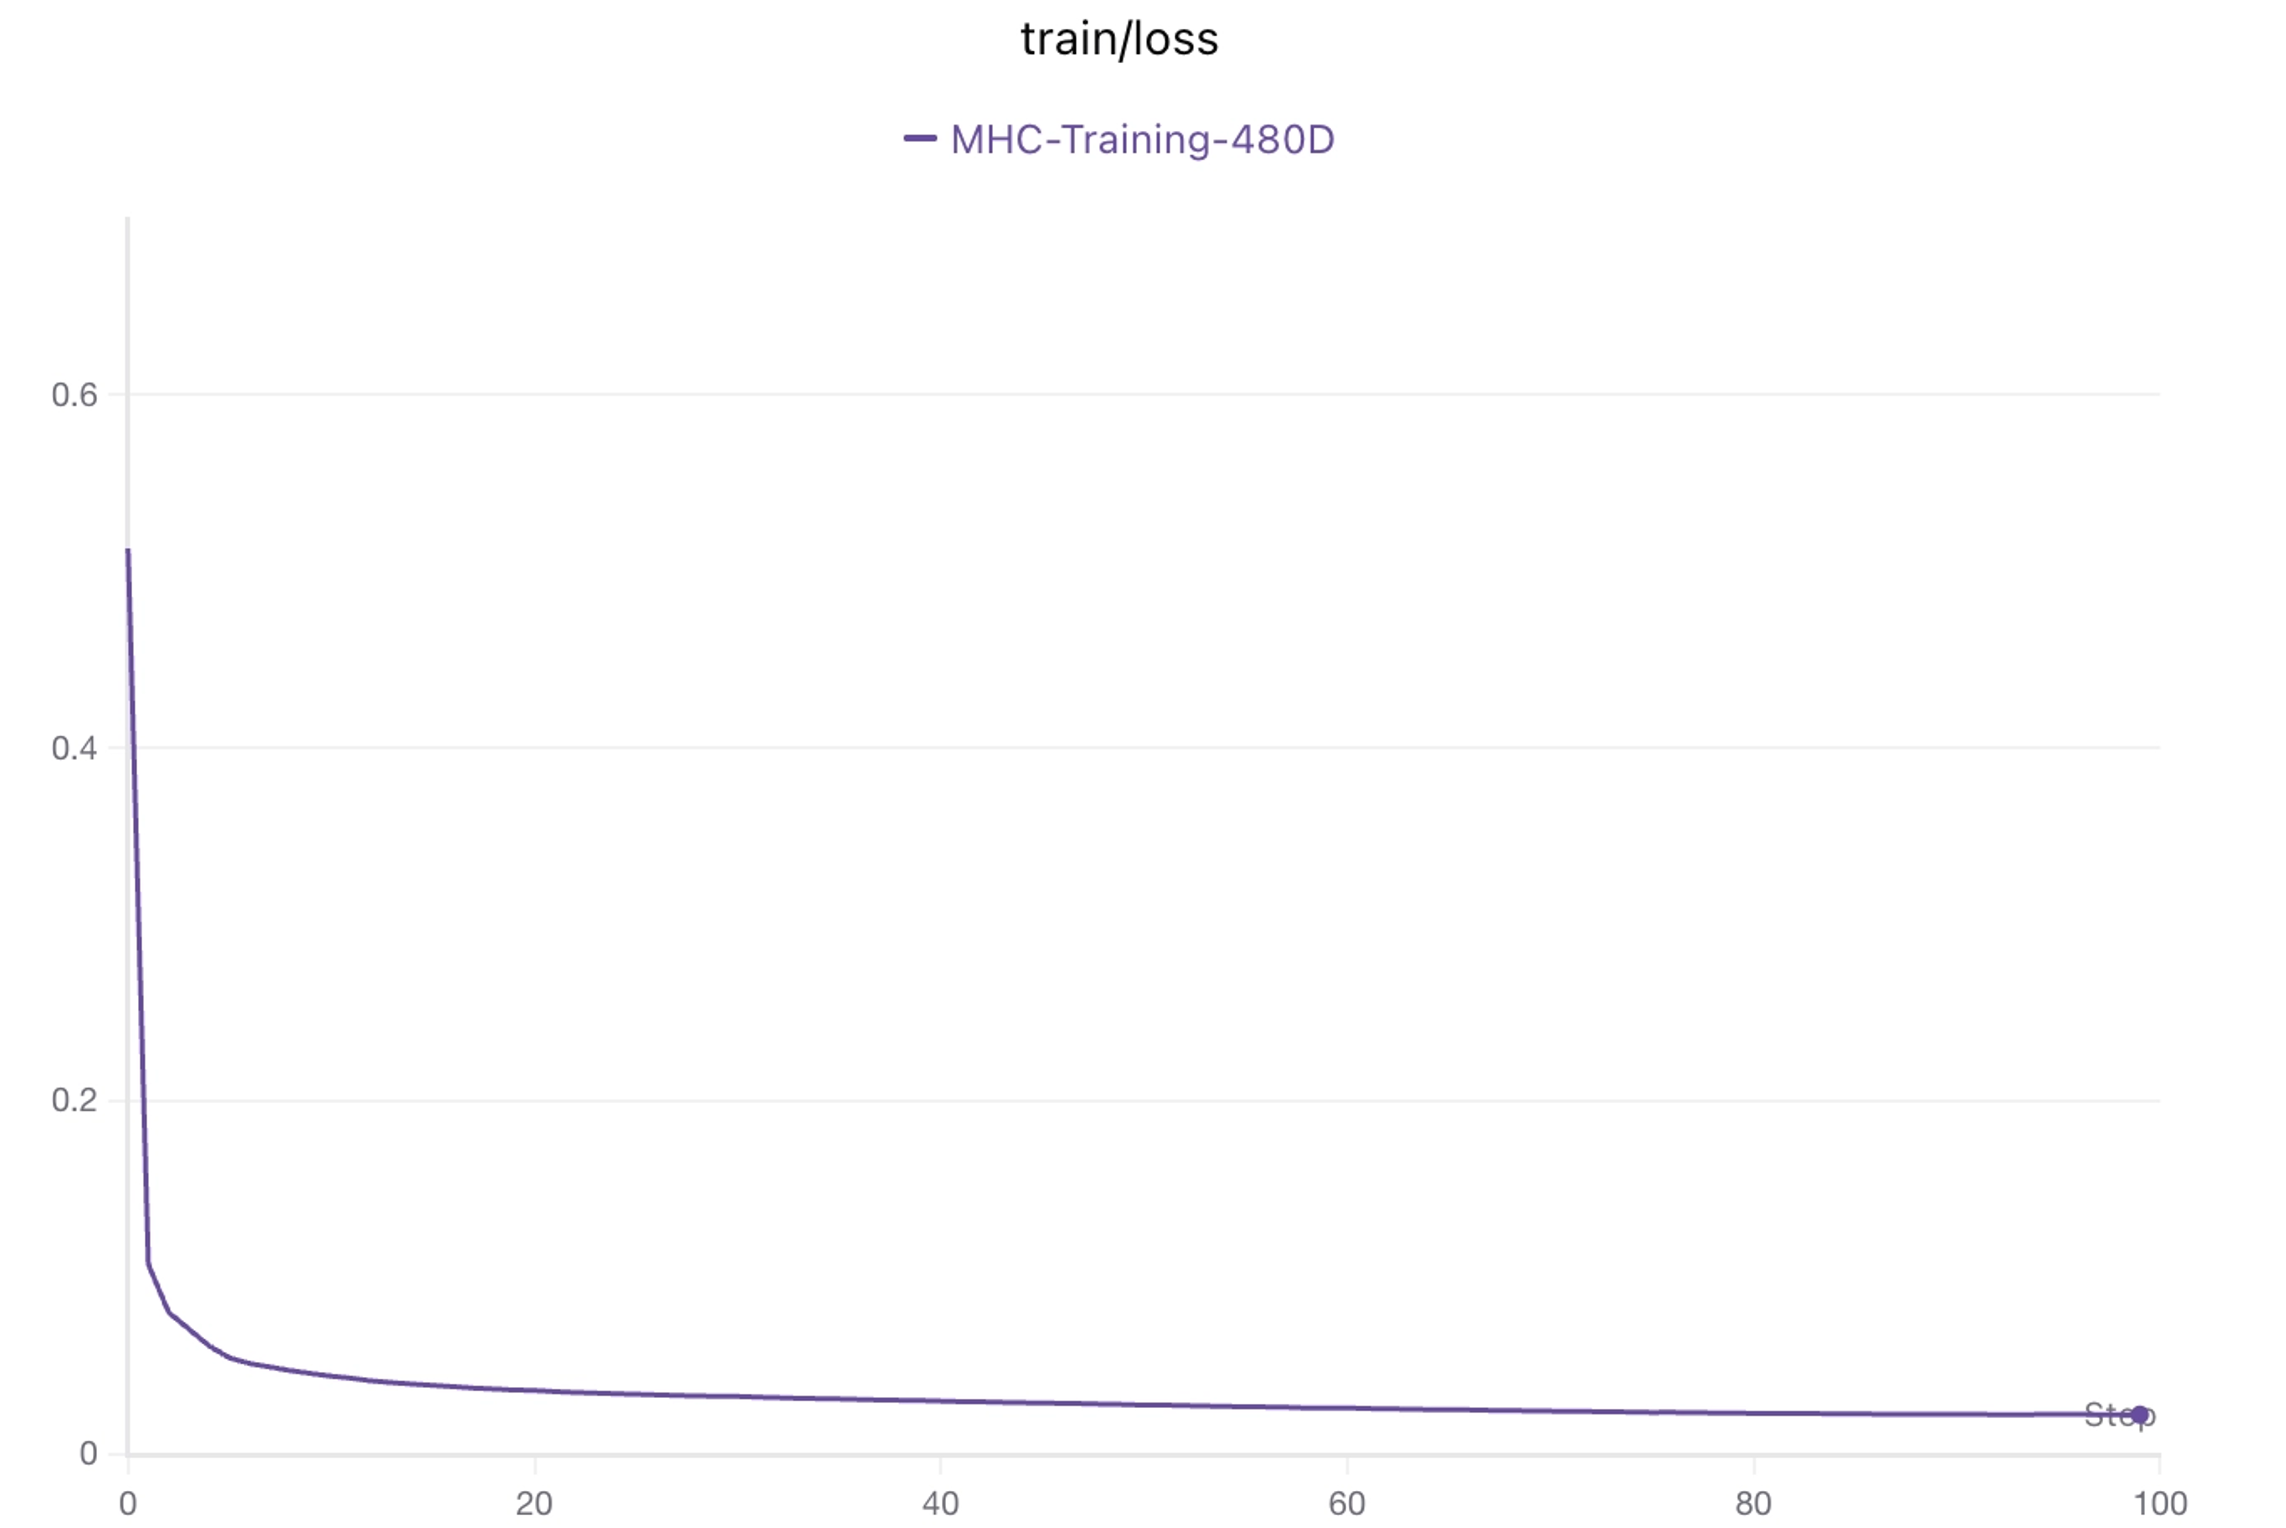
\includegraphics[width=0.70\textwidth]{figures/training_curve.png}
    \caption{训练过程曲线}
    \label{fig:training-curve}
\end{figure}

图~\ref{fig:training-curve} 绘制了训练过程中的主要指标曲线。整体趋势显示模型训练过程平稳，测试指标未见显著异常波动，表明实验环境与复现流程能够支撑后续的模型优化实验。

\subsection{任务设置}

实验围绕 FennOmix.MHC 的复现与部署优化展开，涵盖四类主要任务：其一，复现原始模型的训练和测试流程；其二，考察不同输出维度对模型性能及缓存成本的影响；其三，比较 Linear 与 MLP 两种 64 维降维模型在常规指标和下游缩库辅助搜库任务中的表现；其四，检验剪枝、INT8 量化压缩以及索引加载机制对系统部署的作用。

在大规模部署背景下，考虑将人类常见蛋白质序列切割为长度 8--14 mer 的候选肽段，按此策略，候选肽段的总量约为 7300 万条。

\subsection{评价指标设置}

为全面衡量模型优化前后的性能变化，本文采用两类核心指标。第一类是基于排名阈值的召回率，包含 rank@0.1、rank@0.5 和 rank@2.0，用于评估模型将真实结合肽段排在候选结果前列的能力。第二类是基于欧氏距离阈值的召回率，包含 dist@0.2、dist@0.3 和 dist@0.4，用于衡量 HLA 与真实结合肽段在共享嵌入空间中的邻近程度。

此外，为评价降维模型在真实应用场景中的表现，本文还引入第~\ref{sec:direct-model-search} 节所述的缩库辅助数据库检索任务，对 Direct Search 与 Model-assisted Search 的结果实施 overlap 分析，并借助 Precision-like、Recall-like、Overlap-F1、Loss Rate、Expansion Rate 和 Comprehensive Score 六项指标进行综合比较。

\section{不同输出维度实验结果分析}

% \begin{figure}[htbp]
%     \centering
%     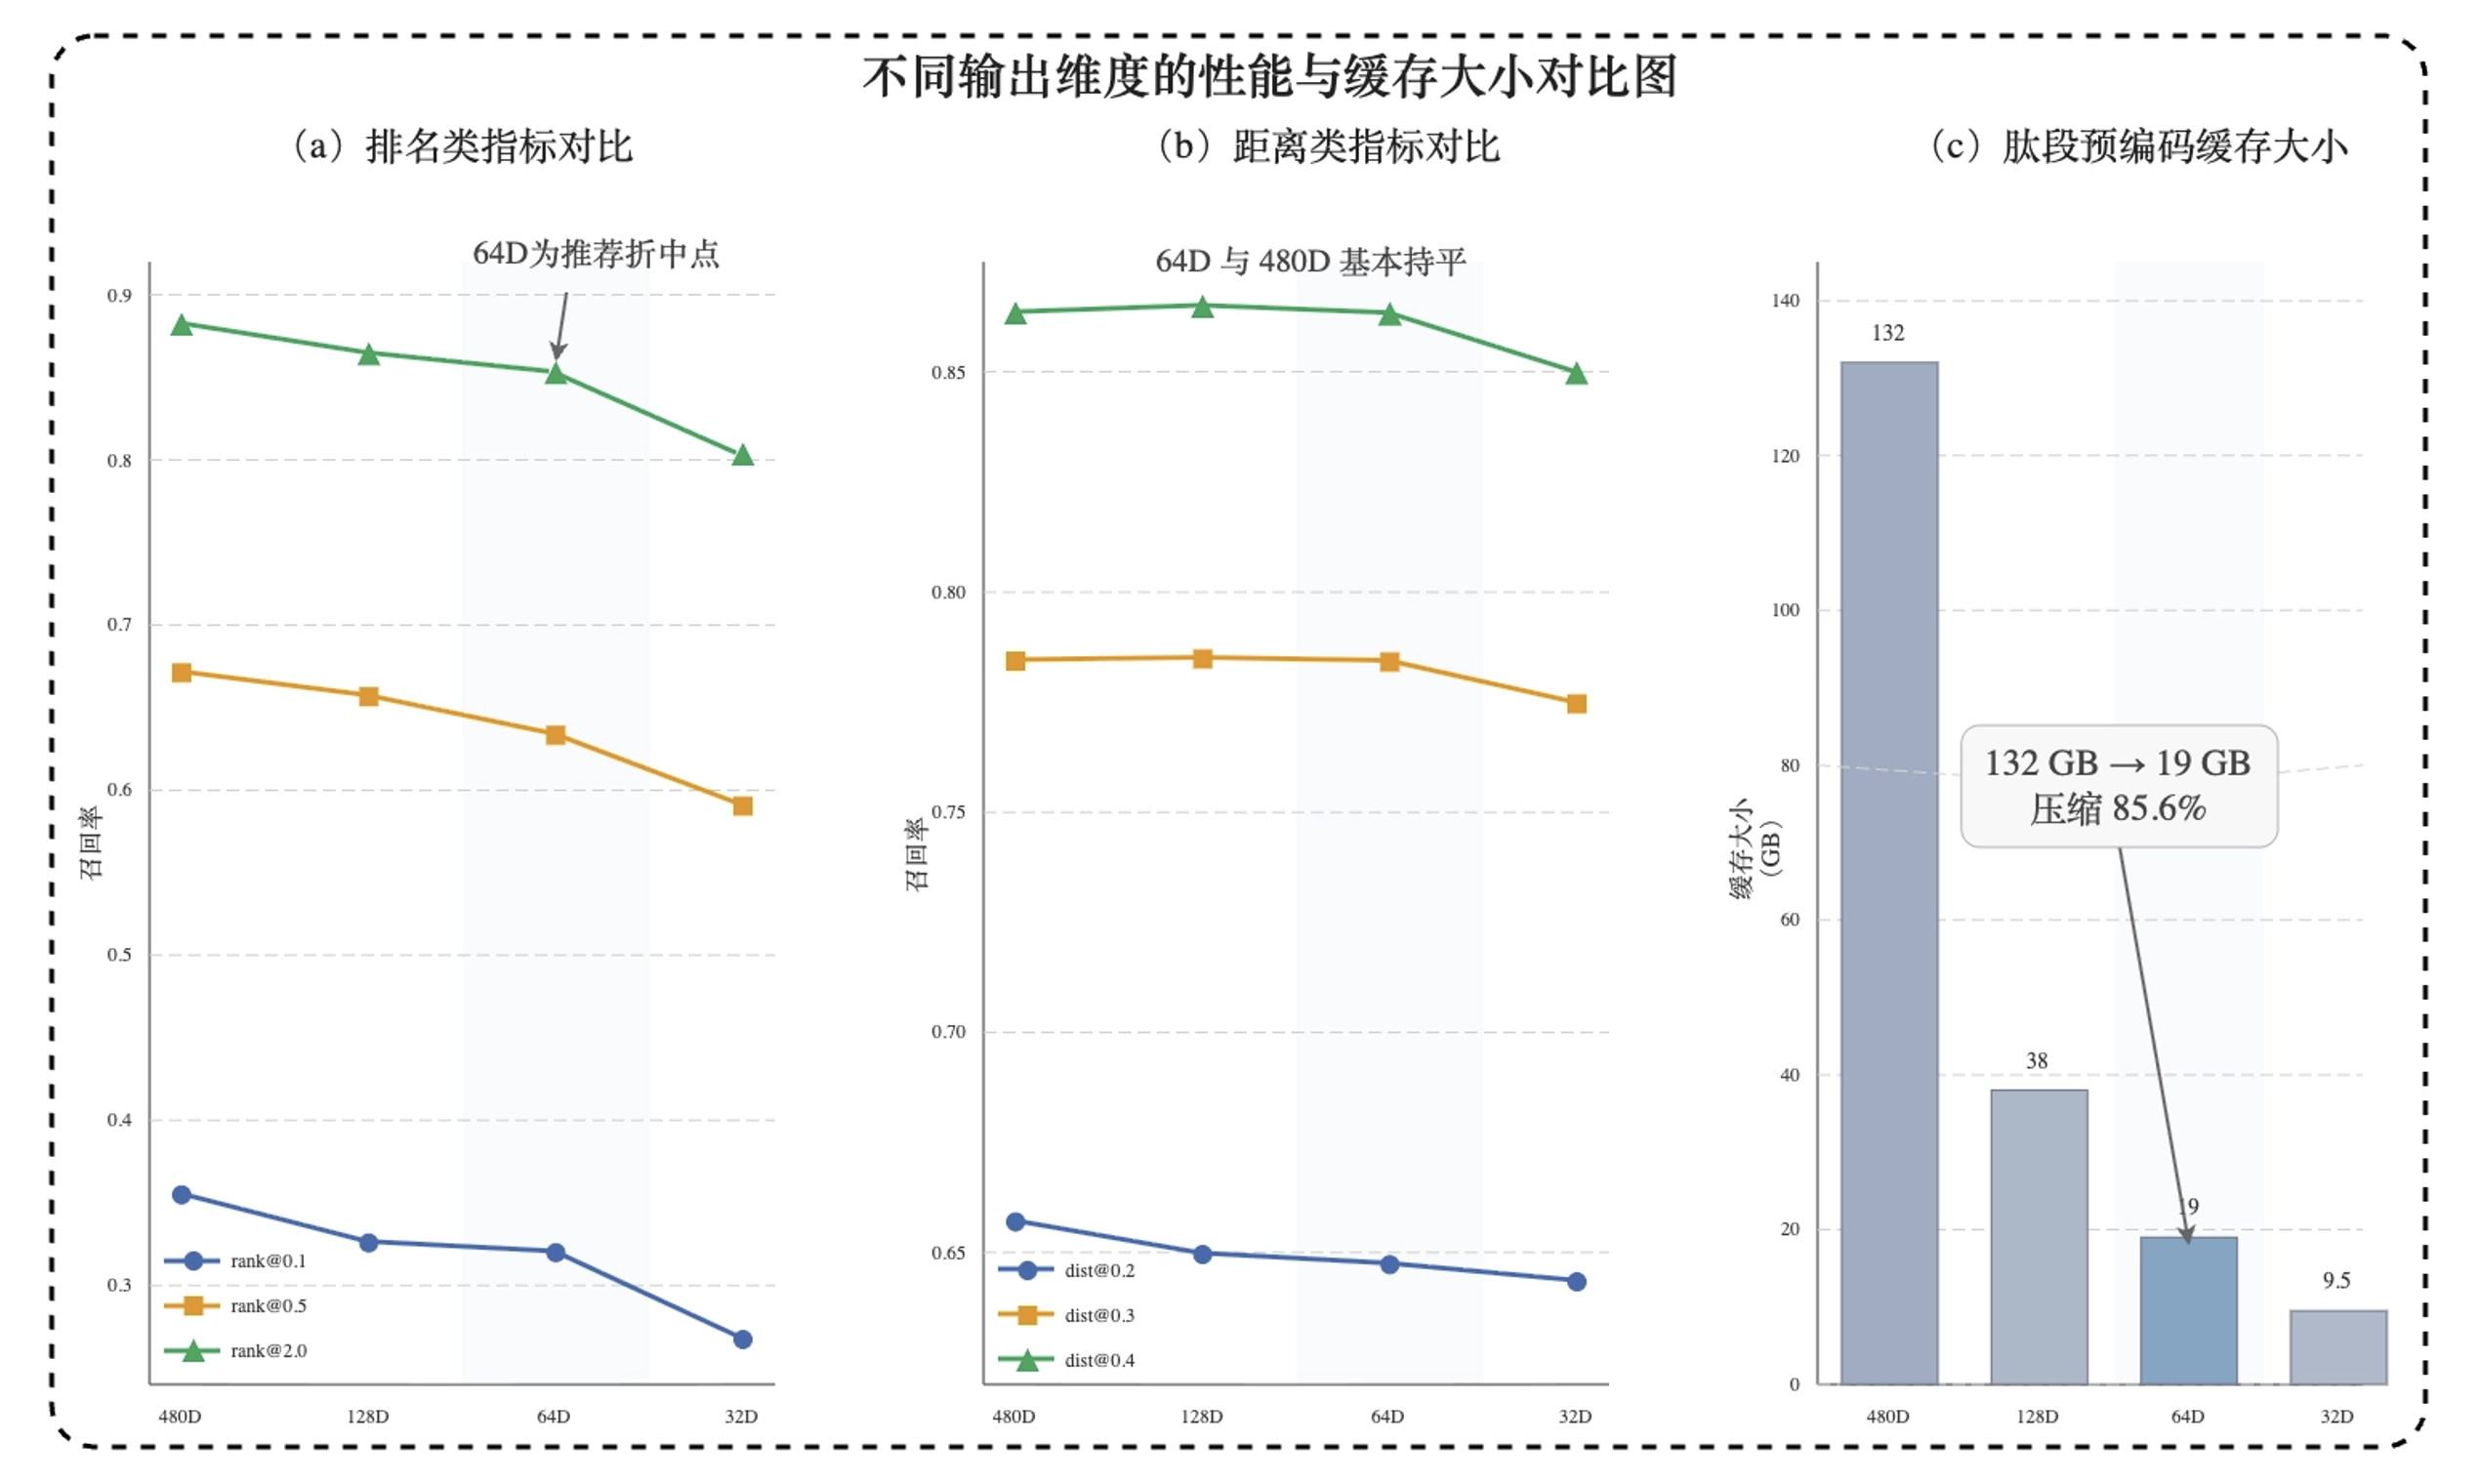
\includegraphics[width=0.90\textwidth]{figures/dimension_comparison.png}
%     \caption{不同输出维度综合比较图}
%     \label{fig:dimension-comparison}
% \end{figure}

\subsection{不同维度模型的整体性能比较}

为分析输出维度对模型性能的影响，本文比对了 480D、128D、64D 和 32D 四种配置在 rank-recall 与 distance-recall 指标上的表现，结果汇总于表~\ref{tab:dimension-performance}。

\begin{table}[htbp]
    \centering
    \caption{不同输出维度模型性能比较}
    \label{tab:dimension-performance}
    \begin{tabular}{ccccccc}
        \toprule
        输出维度 & rank@0.1 & rank@0.5 & rank@2.0 & dist@0.2 & dist@0.3 & dist@0.4 \\
        \midrule
        480D & 0.3548 & 0.6710 & 0.8820 & 0.6569 & 0.7843 & 0.8633 \\
        128D & 0.3257 & 0.6566 & 0.8641 & 0.6495 & 0.7848 & 0.8648 \\
        64D  & 0.3198 & 0.6332 & 0.8460 & 0.6472 & 0.7841 & 0.8631 \\
        32D  & 0.2672 & 0.5903 & 0.8820 & 0.6433 & 0.7746 & 0.8497 \\
        \bottomrule
    \end{tabular}
\end{table}

从 rank-recall 来看，随输出维度逐步压缩，rank@0.1 和 rank@0.5 整体呈现下降趋势，表明维度缩减会在一定程度上削弱模型对高优先级候选肽段的排序质量。其中，32D 的降幅更为明显，提示过度的压缩可能损害模型对细粒度候选差异的分辨力。

从 distance-recall 来看，128D 和 64D 与原始 480D 之间的差距很小，尤其在 dist@0.3 和 dist@0.4 两项上几乎持平。64D 模型的 dist@0.3 为 0.7841，与 480D 的 0.7843 极为接近；dist@0.4 为 0.8631，与 480D 的 0.8633 也基本一致，说明 64D 虽降低了表示维度，但仍较完整地维持了原始共享嵌入空间的邻域结构。

\begin{figure}[htbp]
    \centering
    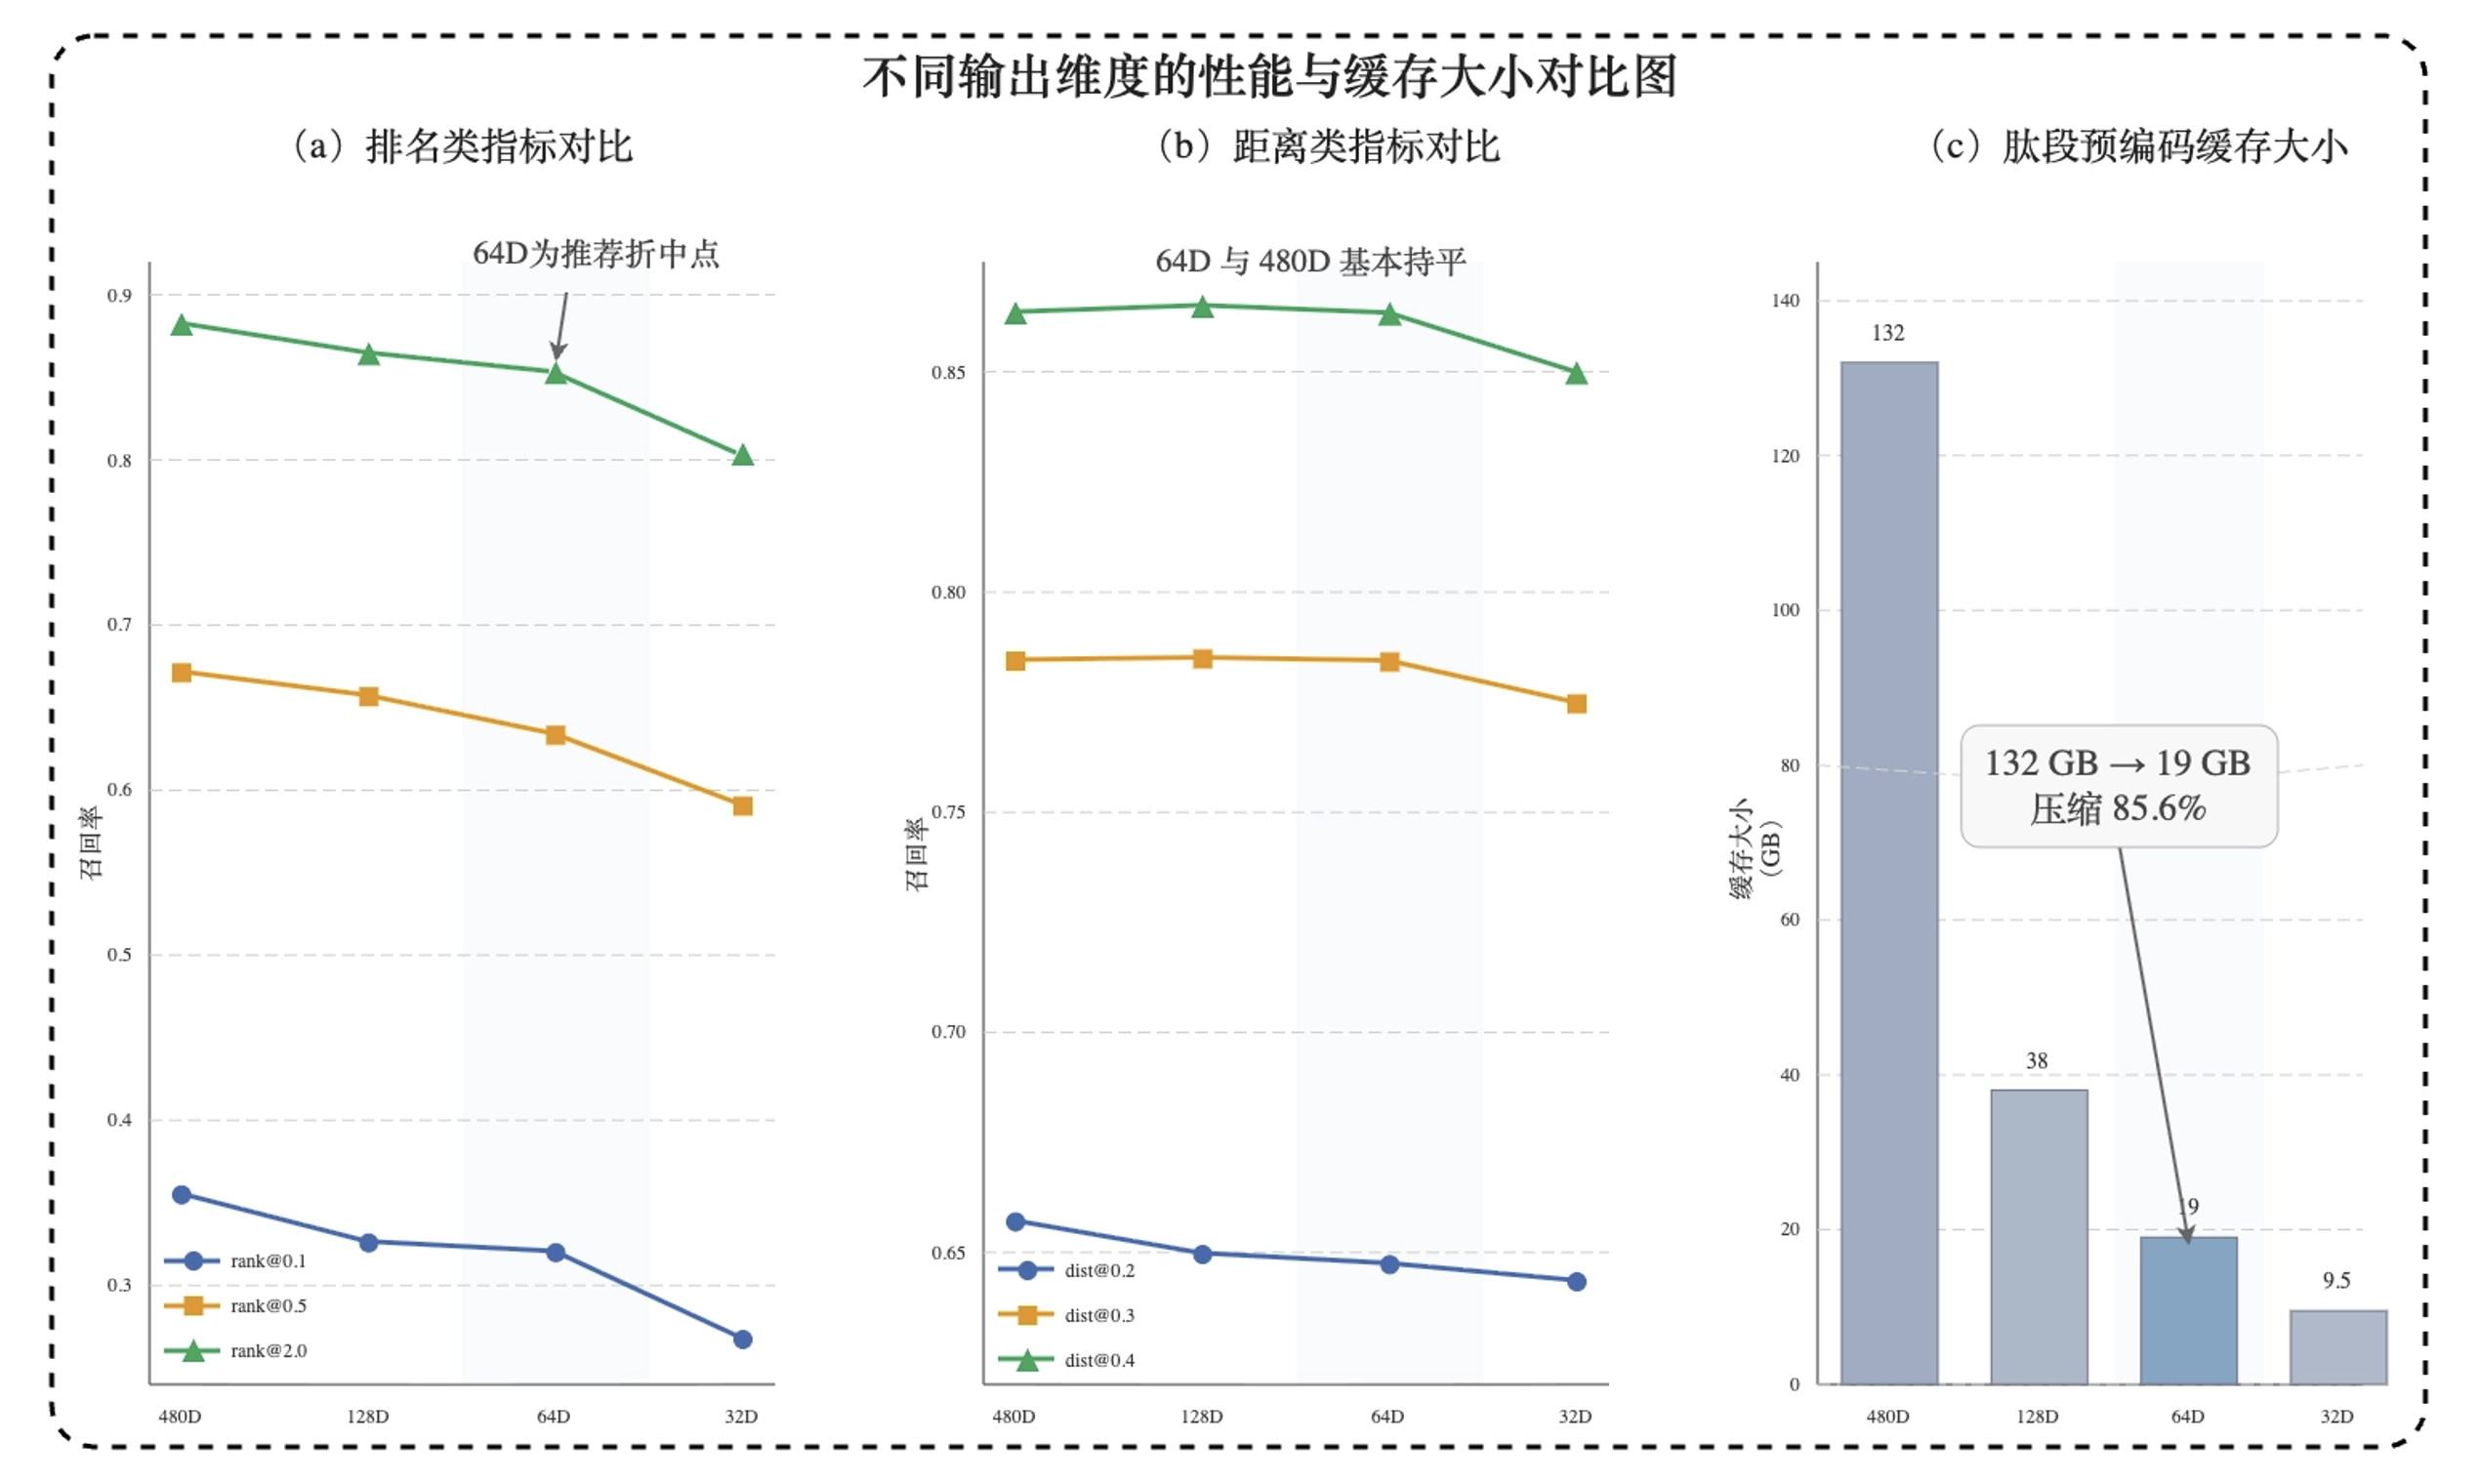
\includegraphics[width=0.90\textwidth]{figures/dimension_comparison.png}
    \caption{不同输出维度综合比较图}
    \label{fig:dimension-comparison}
\end{figure}

\subsection{不同维度模型的缓存成本比较}

除预测性能外，缓存规模是本文关切的另一项核心指标。表~\ref{tab:dimension-cache-size} 列出了不同输出维度下肽段预编码缓存的规模。

\begin{table}[htbp]
    \centering
    \caption{不同输出维度对应缓存规模比较}
    \label{tab:dimension-cache-size}
    \begin{tabular}{ccc}
        \toprule
        输出维度 & 缓存规模 & 相对 480D 的变化 \\
        \midrule
        480D & 132 GB & 基准 \\
        128D & 38 GB  & 明显降低 \\
        64D  & 19 GB  & 降低约 85.6\% \\
        32D  & 9.5 GB & 进一步降低 \\
        \bottomrule
    \end{tabular}
\end{table}

可见，输出维度与缓存规模基本呈线性关系。480D 模型约 132 GB 的缓存体积难以直接适配普通单机部署；128D 可将缓存压缩至 38 GB，但存储和加载成本仍然偏高；64D 进一步降至 19 GB，在资源占用上已明显更适合部署；32D 虽缓存最小，但需权衡前述性能上的损失。

\subsection{64 维方案的综合优势分析}

\begin{figure}[htbp]
    \centering
    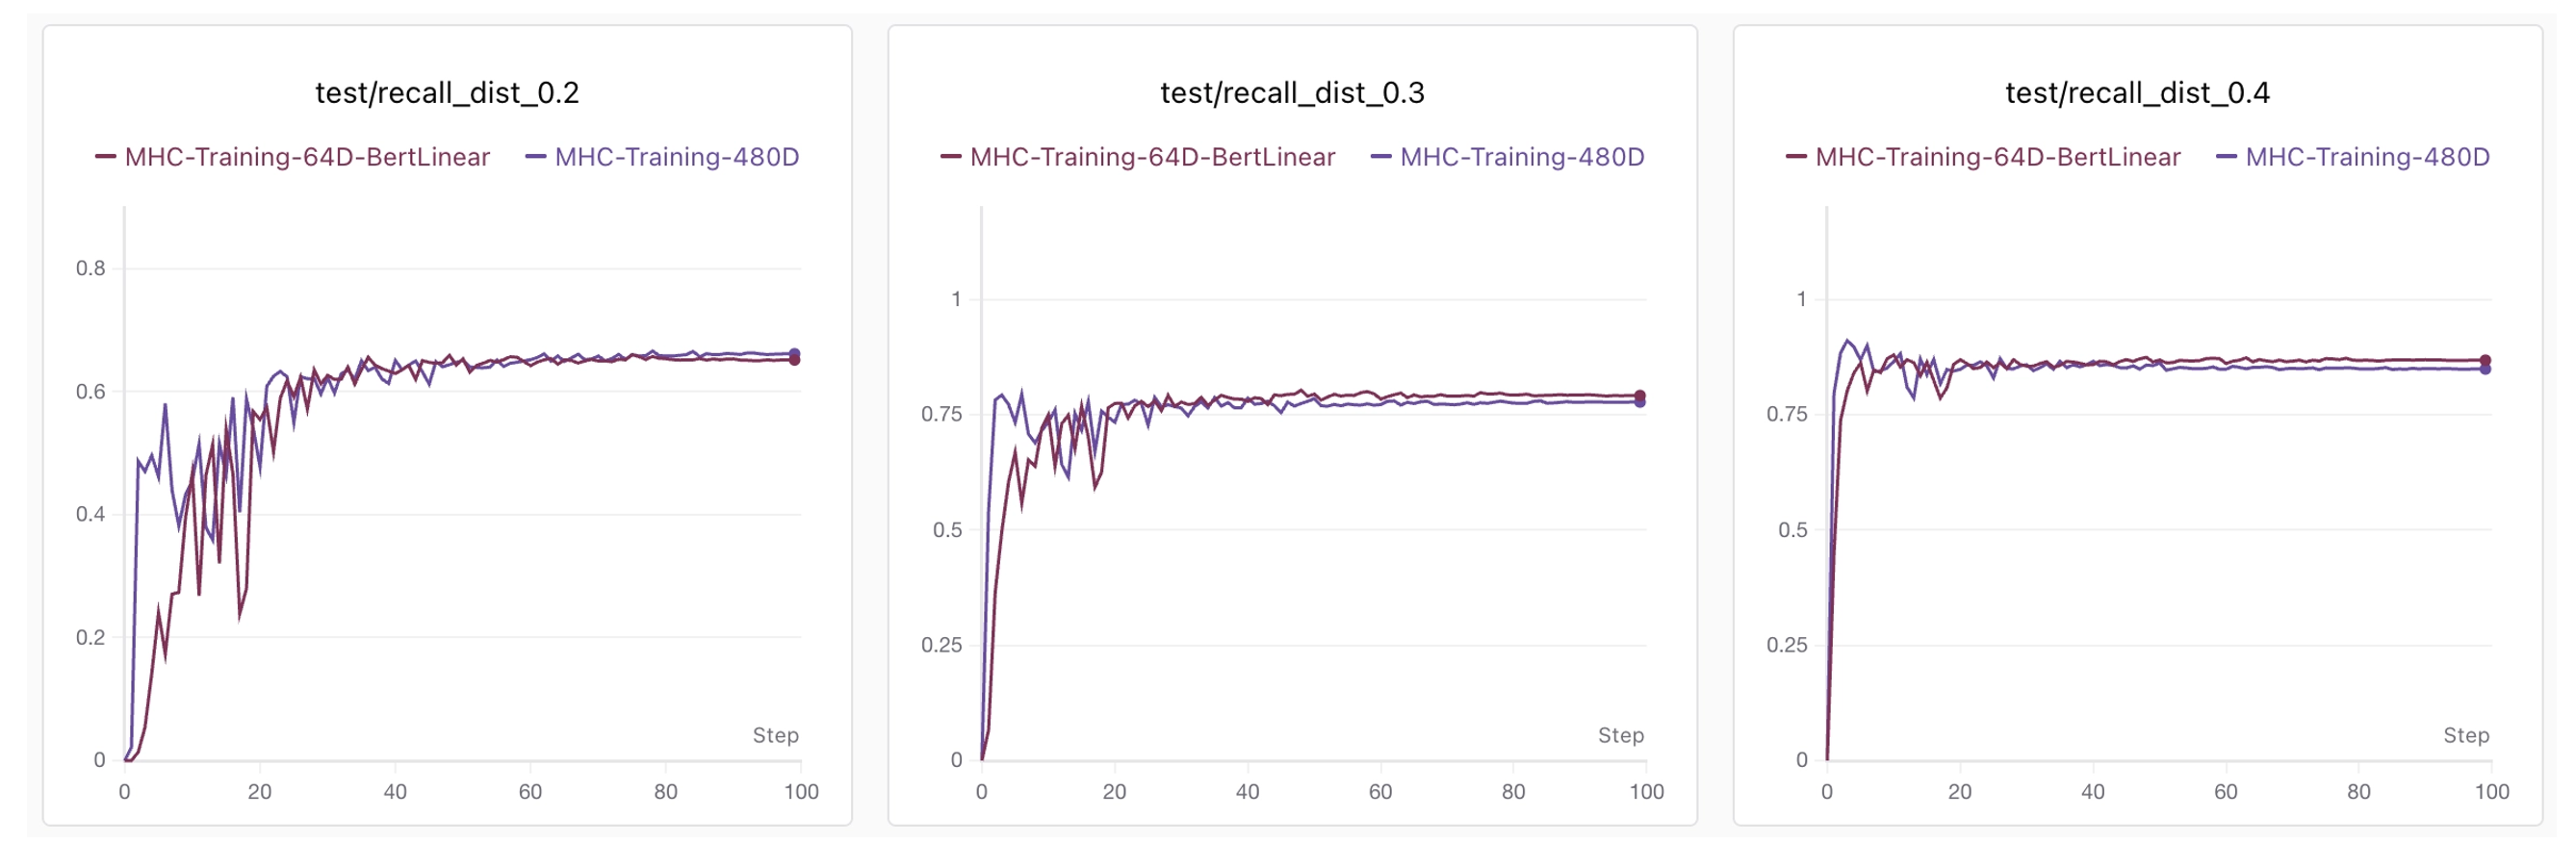
\includegraphics[width=1.0\textwidth]{figures/64d_vs_480d.png}
    \caption{64D 方案相对 480D 的压缩与 recall\_dist\_0.3 性能比较图}
    \label{fig:64d-vs-480d}
\end{figure}

综合性能与缓存成本来看，64D 是当前实验条件下较优的输出维度。一方面，它将缓存规模从 132 GB 压缩至 19 GB，显著缓解了大规模肽段库的存储压力；另一方面，其 distance-recall 指标与 480D 几无差别，说明模型的核心空间结构保持稳定。

与 128D 相比，64D 在性能损失可控的条件下额外削减了约一半缓存体积；与 32D 相比，64D 虽缓存略大，但模型表现更稳健。因此，64D 在“性能保持”与“存储压缩”之间取得了更合理的平衡。基于这一结论，后续的 Linear/MLP 对比、剪枝实验以及缓存压缩实验均以 64D 模型作为主要研究对象。

\section{线性与非线性降维模型比较分析}

\subsection{实验目的与比较对象}

在确定 64D 为主要压缩目标后，本文进一步对比 MHC-64D-BertLinear 与 MHC-64D-BertMLP 两种降维模型。两类模型的结构已在第 3.3 节中说明，此处不再赘述，而将重点放在二者在常规预测指标和下游缩库辅助搜库任务中的实验表现上。

本实验旨在判断：在相同的输出维度下，结构更轻量的 Linear 模型是否即可满足任务需求，还是具备更强非线性表达能力的 MLP 模型能带来额外增益。

\subsection{常规预测指标比较}

MHC-64D-BertLinear、MHC-64D-BertMLP 与原始 MHC-480D 在 Top-0.1\%、Top-0.5\% 和 Top-2.0\% 三个 rank-recall 指标上的整体差异不大。与此同时，在 recall\_dist\_0.2、recall\_dist\_0.3 和 recall\_dist\_0.4 等基于欧氏距离阈值的召回率上，两种 64 维模型与 480D 模型之间同样未表现出明显差距，尤其当阈值从 0.1 放宽至 0.3 后，三者的表现更为接近。

\begin{figure}[htbp]
    \centering
    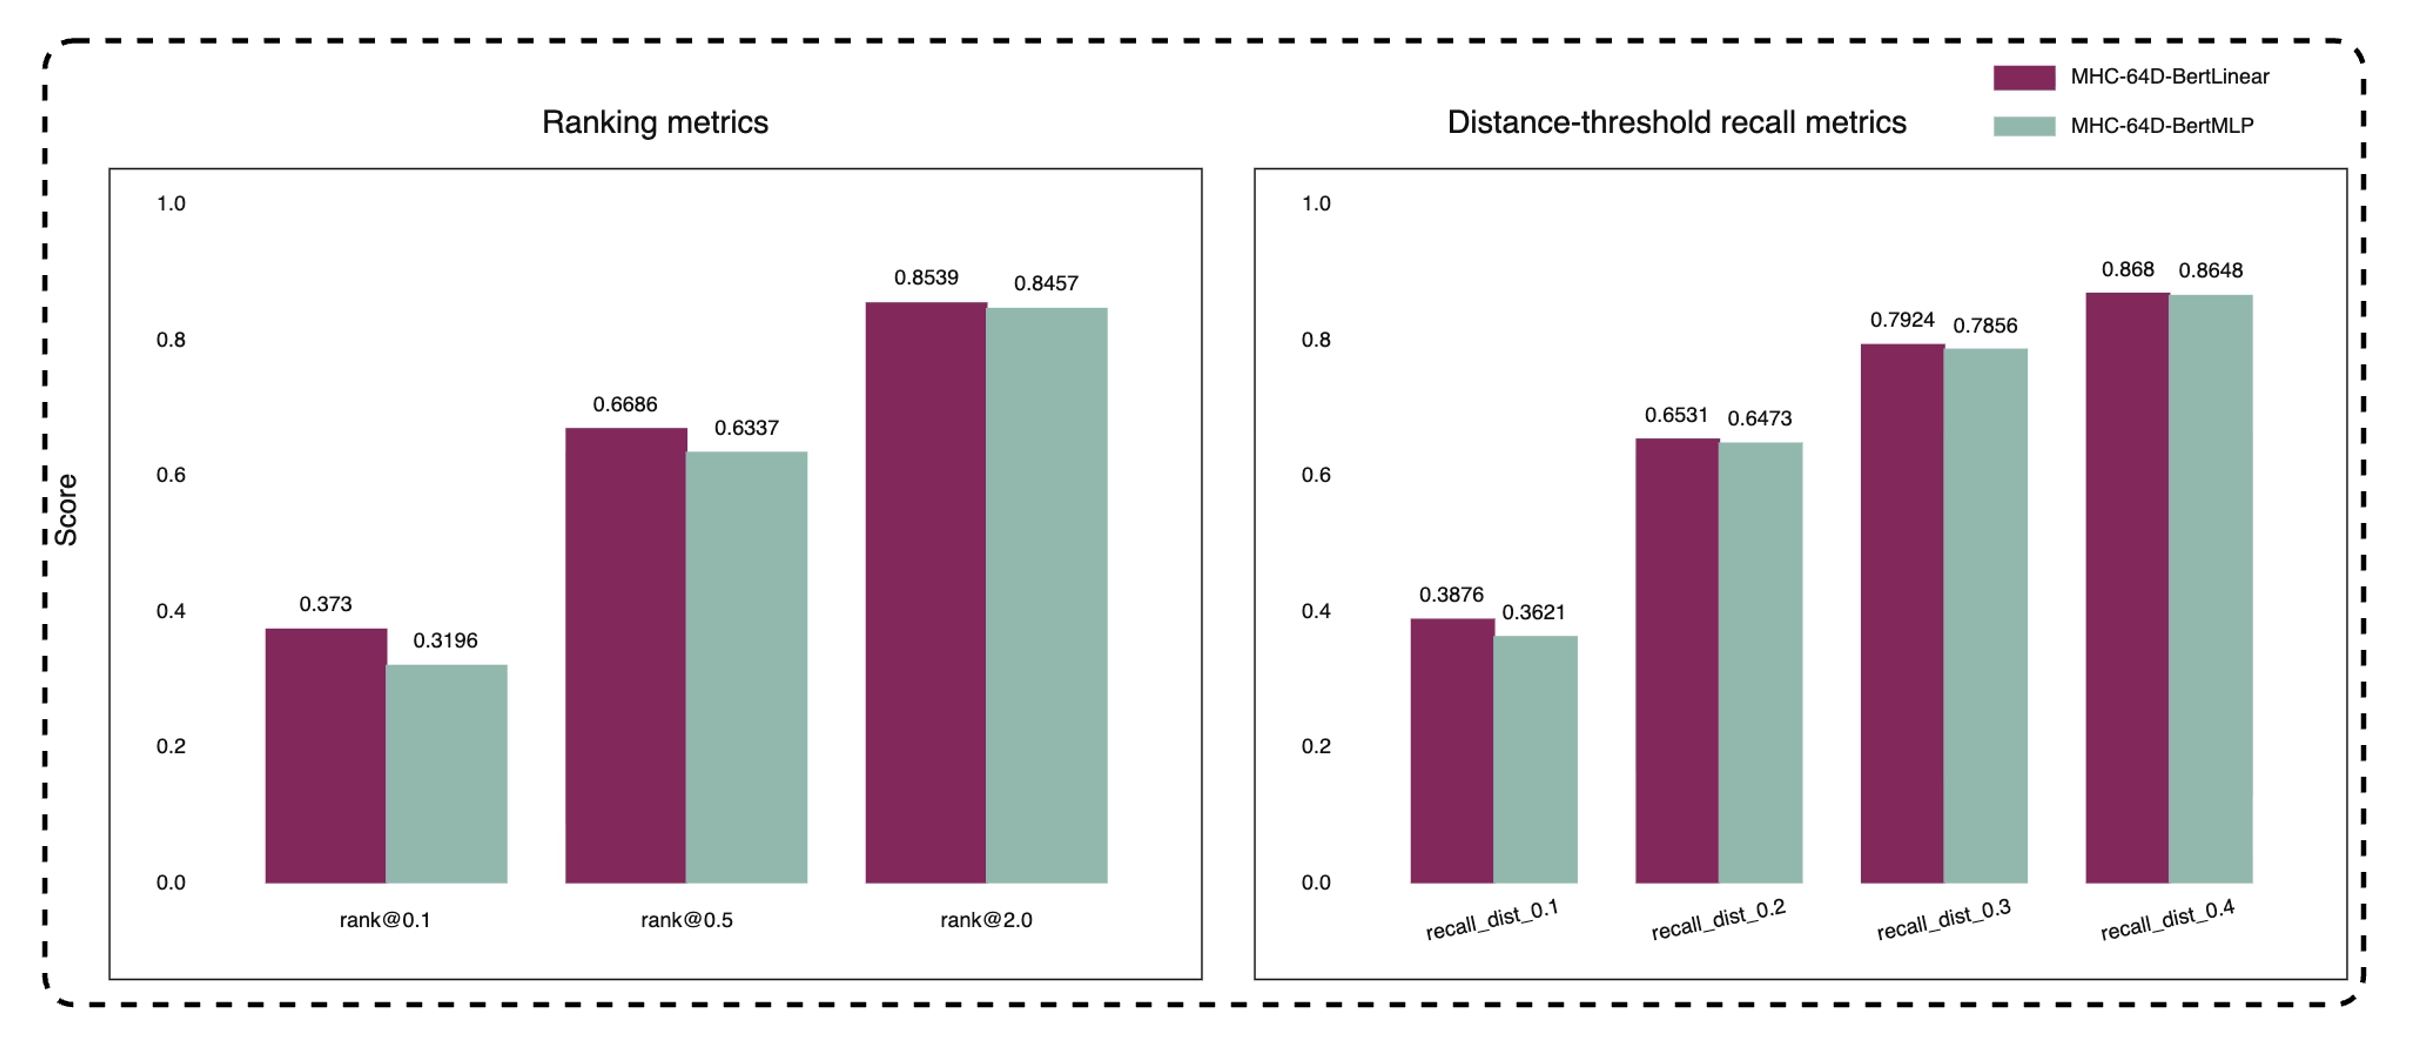
\includegraphics[width=0.85\textwidth]{figures/linear_mlp_metrics.png}
    \caption{Linear 与 MLP 常规指标对比图}
    \label{fig:linear-mlp-metrics}
\end{figure}

图~\ref{fig:linear-mlp-metrics} 显示，Linear 与 MLP 在常规预测指标上的差别微小，两者均能在 64 维条件下维持较好的候选筛选能力和嵌入空间结构。这说明，对当前 FennOmix.MHC 的特征表示而言，64 维已足以承载主要任务信息，更复杂的非线性映射并未在常规指标上体现出明显优势。

因此，仅凭 rank-recall 和 distance-recall 等常规指标，Linear 与 MLP 两类降维策略均具备可用性，二者的优劣还需结合下游缩库辅助搜库任务加以判定。

\subsection{下游缩库辅助搜库结果比较}

\begin{figure}[htbp]
    \centering
    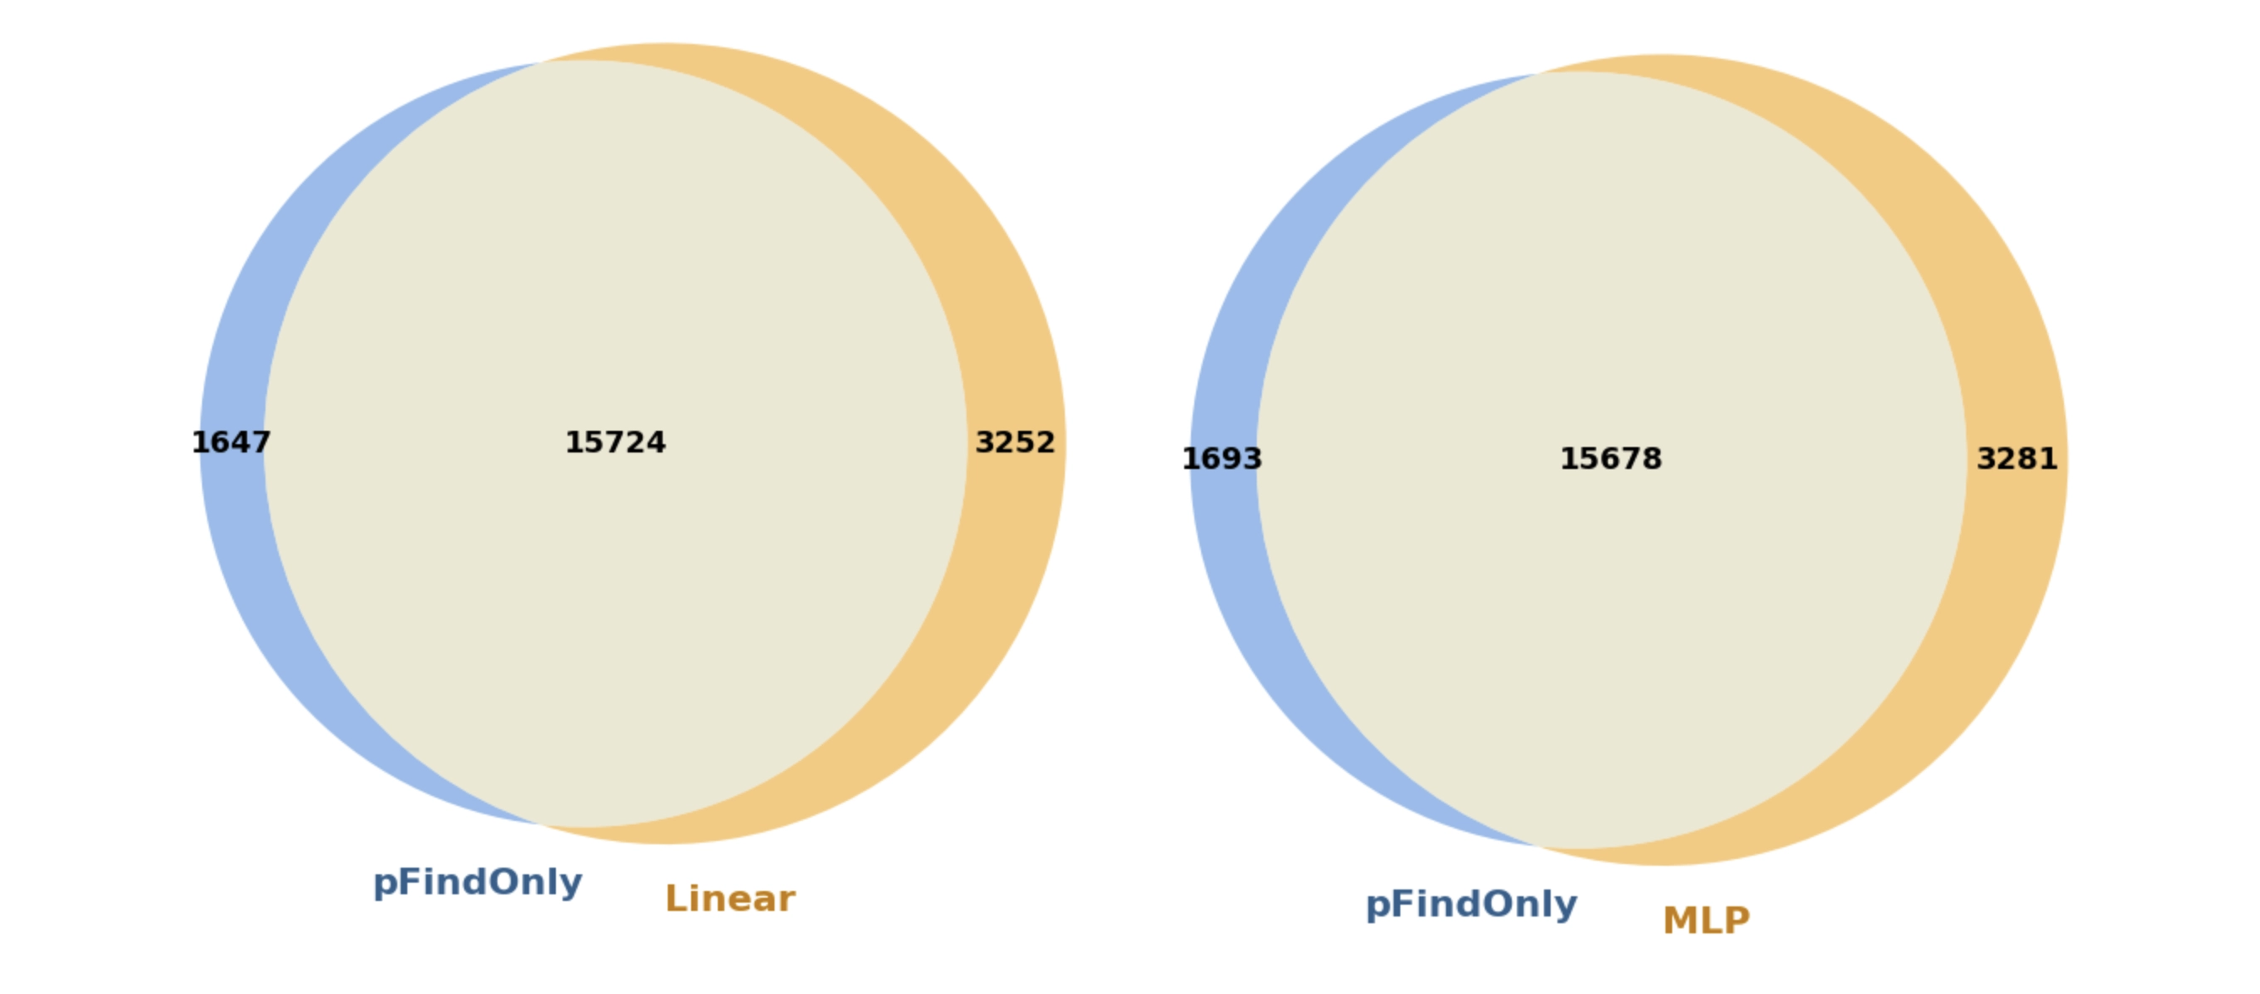
\includegraphics[width=0.85\textwidth]{figures/downstream_search_result.png}
    \caption{下游缩库辅助肽段搜库结果对比图}
    \label{fig:downstream-search-result}
\end{figure}

为更真实地评判两类模型的应用价值，本文进一步引入基于等位基因的缩库辅助数据库检索任务进行对比。具体做法是：对同一批 MS/MS 数据，在已知 HLA 等位基因的条件下分别执行 Direct Search 和 Model-assisted Search 两种流程，后者先由 FennOmix.MHC 对候选肽段进行打分与筛选，构建等位基因特异的缩减数据库，再通过 pFind 实施检索。随后，在肽段层面对两条流程的输出进行 overlap 分析，结果如图~\ref{fig:downstream-search-result} 所示。

\begin{figure}[htbp]
    \centering
    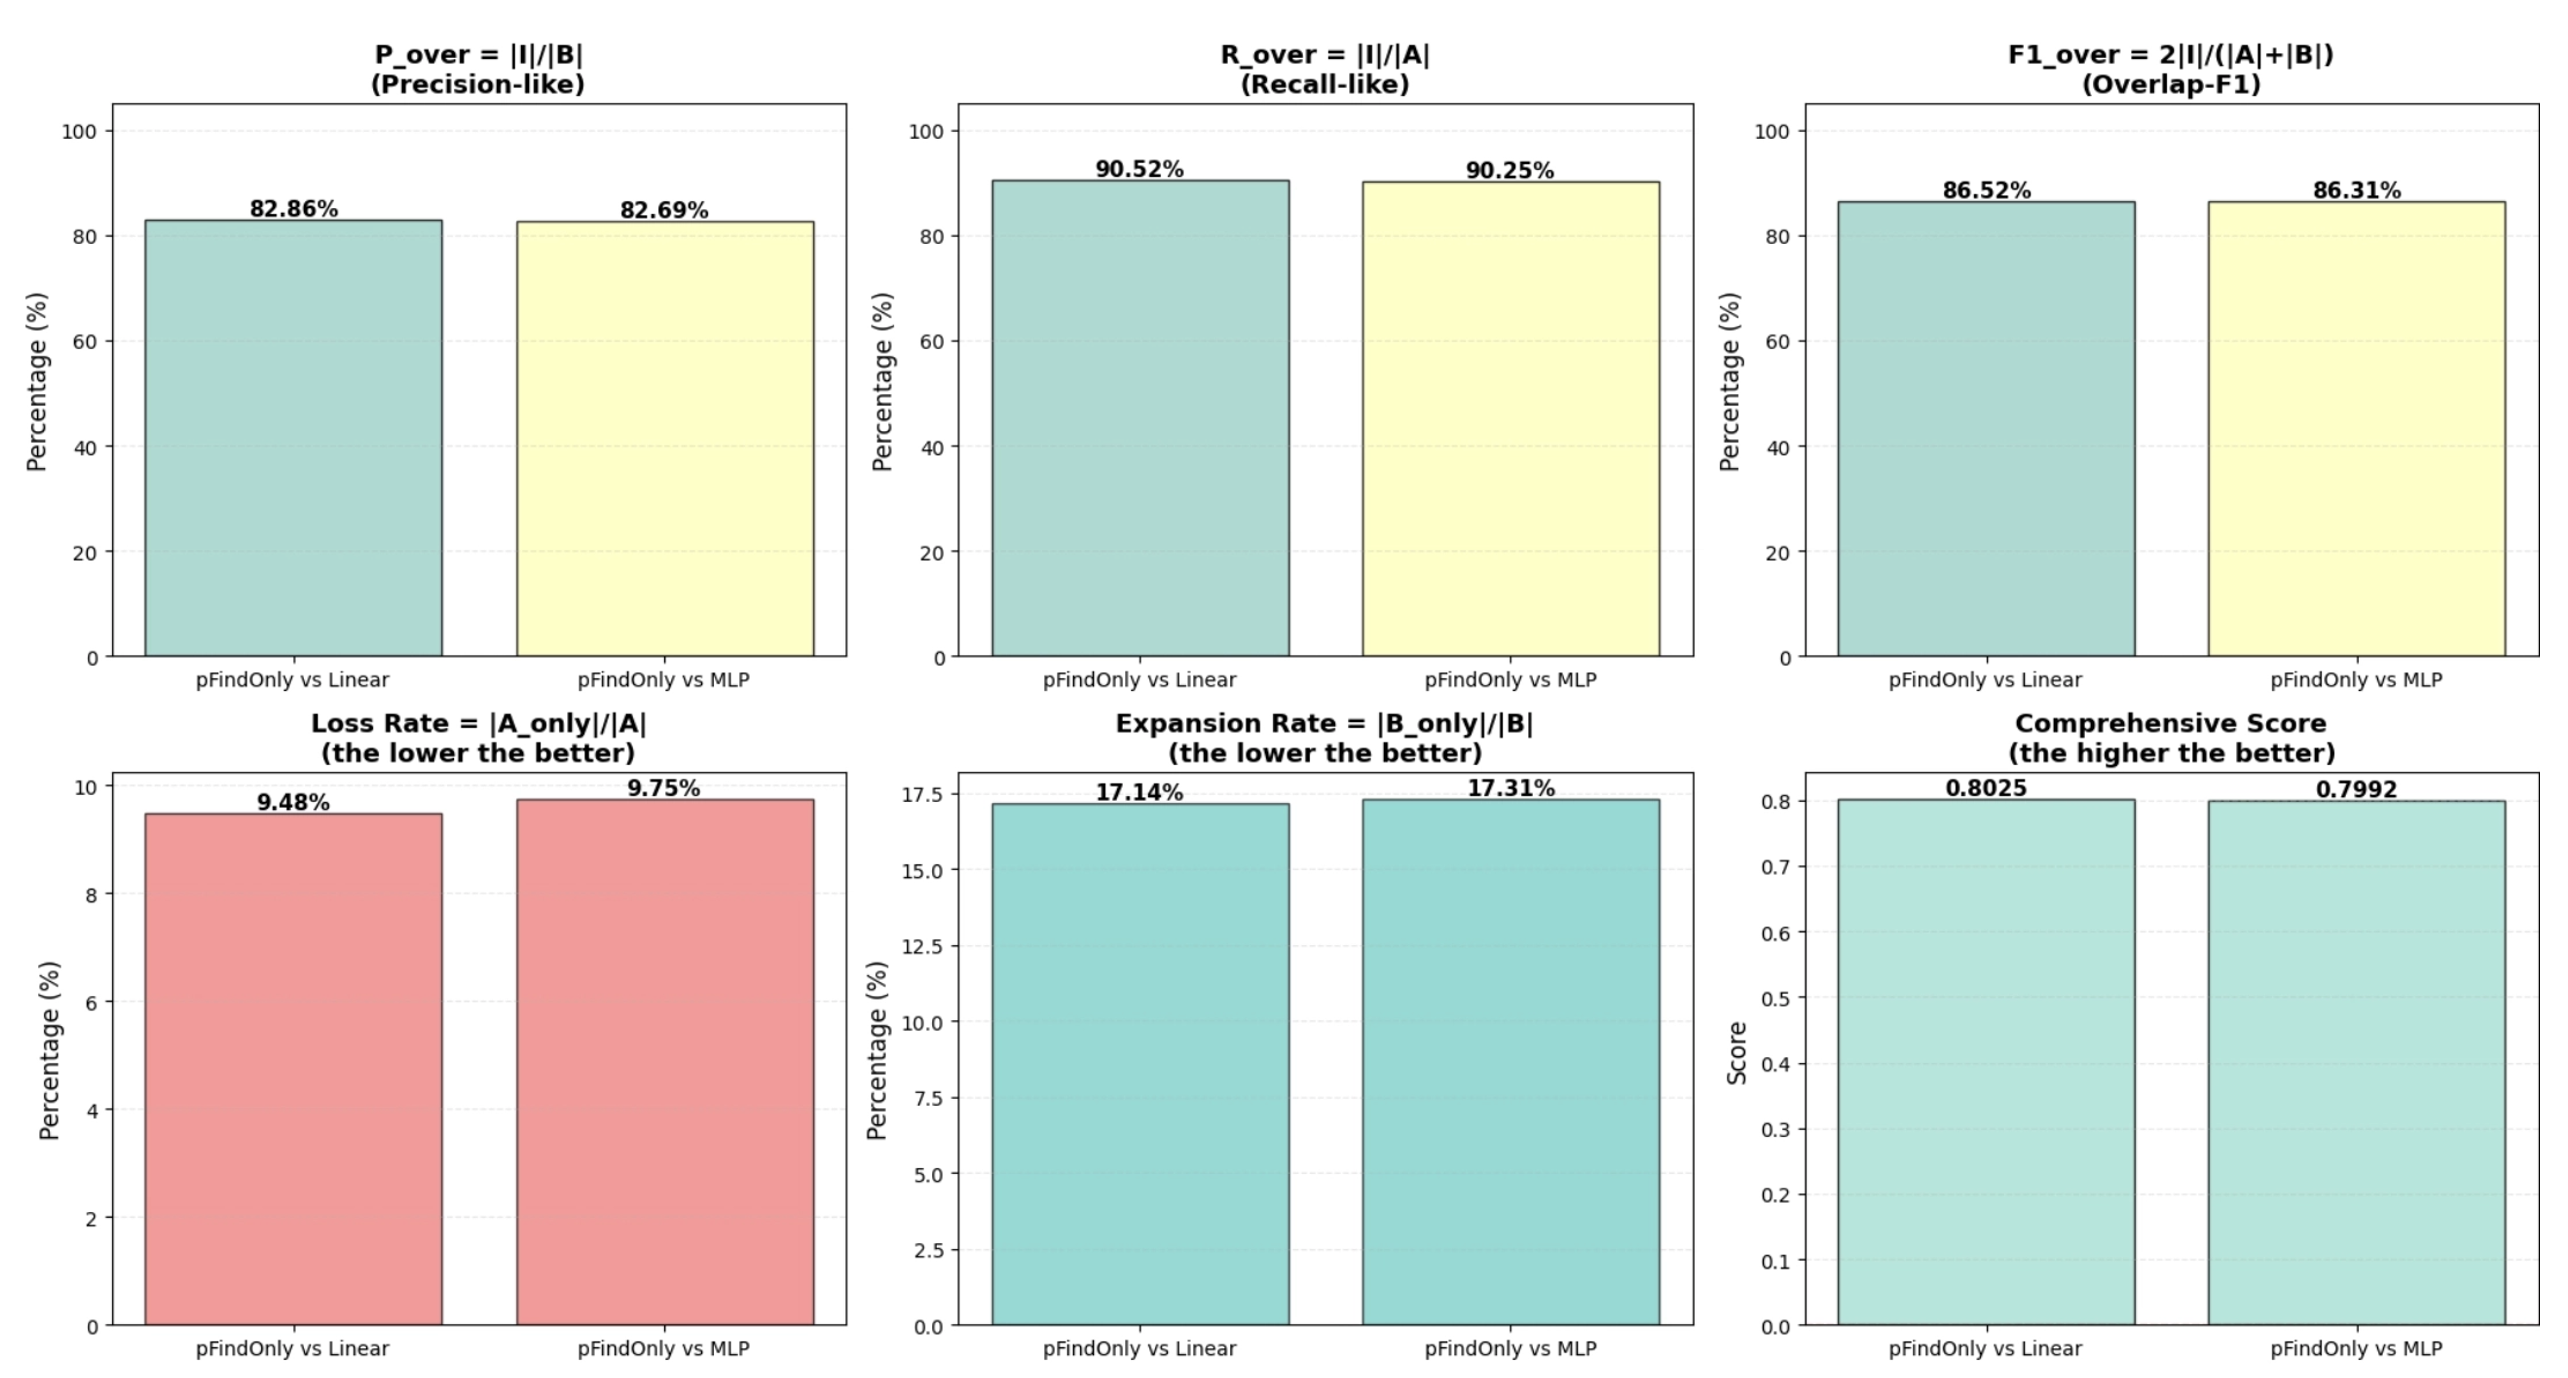
\includegraphics[width=1.0\textwidth]{figures/overlap_scores.png}
    \caption{Linear vs MLP Overlap Scores 指标对比图}
    \label{fig:overlap-scores}
\end{figure}

从图~\ref{fig:overlap-scores} 所示的 Overlap Scores 评价结果来看，Linear 与 MLP 在下游任务中的整体表现相近，但 Linear 在 Precision-like、Recall-like、Overlap-F1、Loss Rate、Expansion Rate 和 Comprehensive Score 六项指标上均呈现出一致的轻微优势。这表明，尽管 MLP 具有更强的非线性表达能力，但在当前任务与数据条件下，这一能力并未转化为更优的下游检索效果。

该结果也印证，当常规预测指标接近时，下游任务评价具有重要参考价值。对于本文所关注的部署场景，模型不仅需要在测试集上维持较好的召回率，还应在真实缩库流程中尽量保留基线检索结果并减少额外差异。Linear 在该任务中的稳健表现，使其更适合被选作默认降维方案。

\subsection{结果分析与结论}

综合常规指标与下游任务结果，Linear 与 MLP 均能在 64D 条件下保持较好的模型性能，但 Linear 在工程部署和应用效果上更具优势：结构更简单、参数量更少、部署成本更低；在常规指标接近的前提下，Linear 在下游 overlap 六项指标中整体略优；且 Linear 的实现与维护更为直接，更适宜作为系统默认模型。

因此，本文最终选定 MHC-64D-BertLinear 作为后续剪枝、缓存压缩与系统部署分析的主要模型基础。

\section{剪枝实验结果分析}

\subsection{剪枝重要性分析结果}

在 64D 线性模型的基础上，本文进一步分析 Transformer 结构中各组件的贡献差异，以判断模型是否存在可剪枝的冗余。实验结果如图~\ref{fig:attention-head-importance} 所示，不同层及不同注意力头的重要性分布并不均衡，表明模型结构中确实存在一定的冗余空间。

\begin{figure}[htbp]
    \centering
    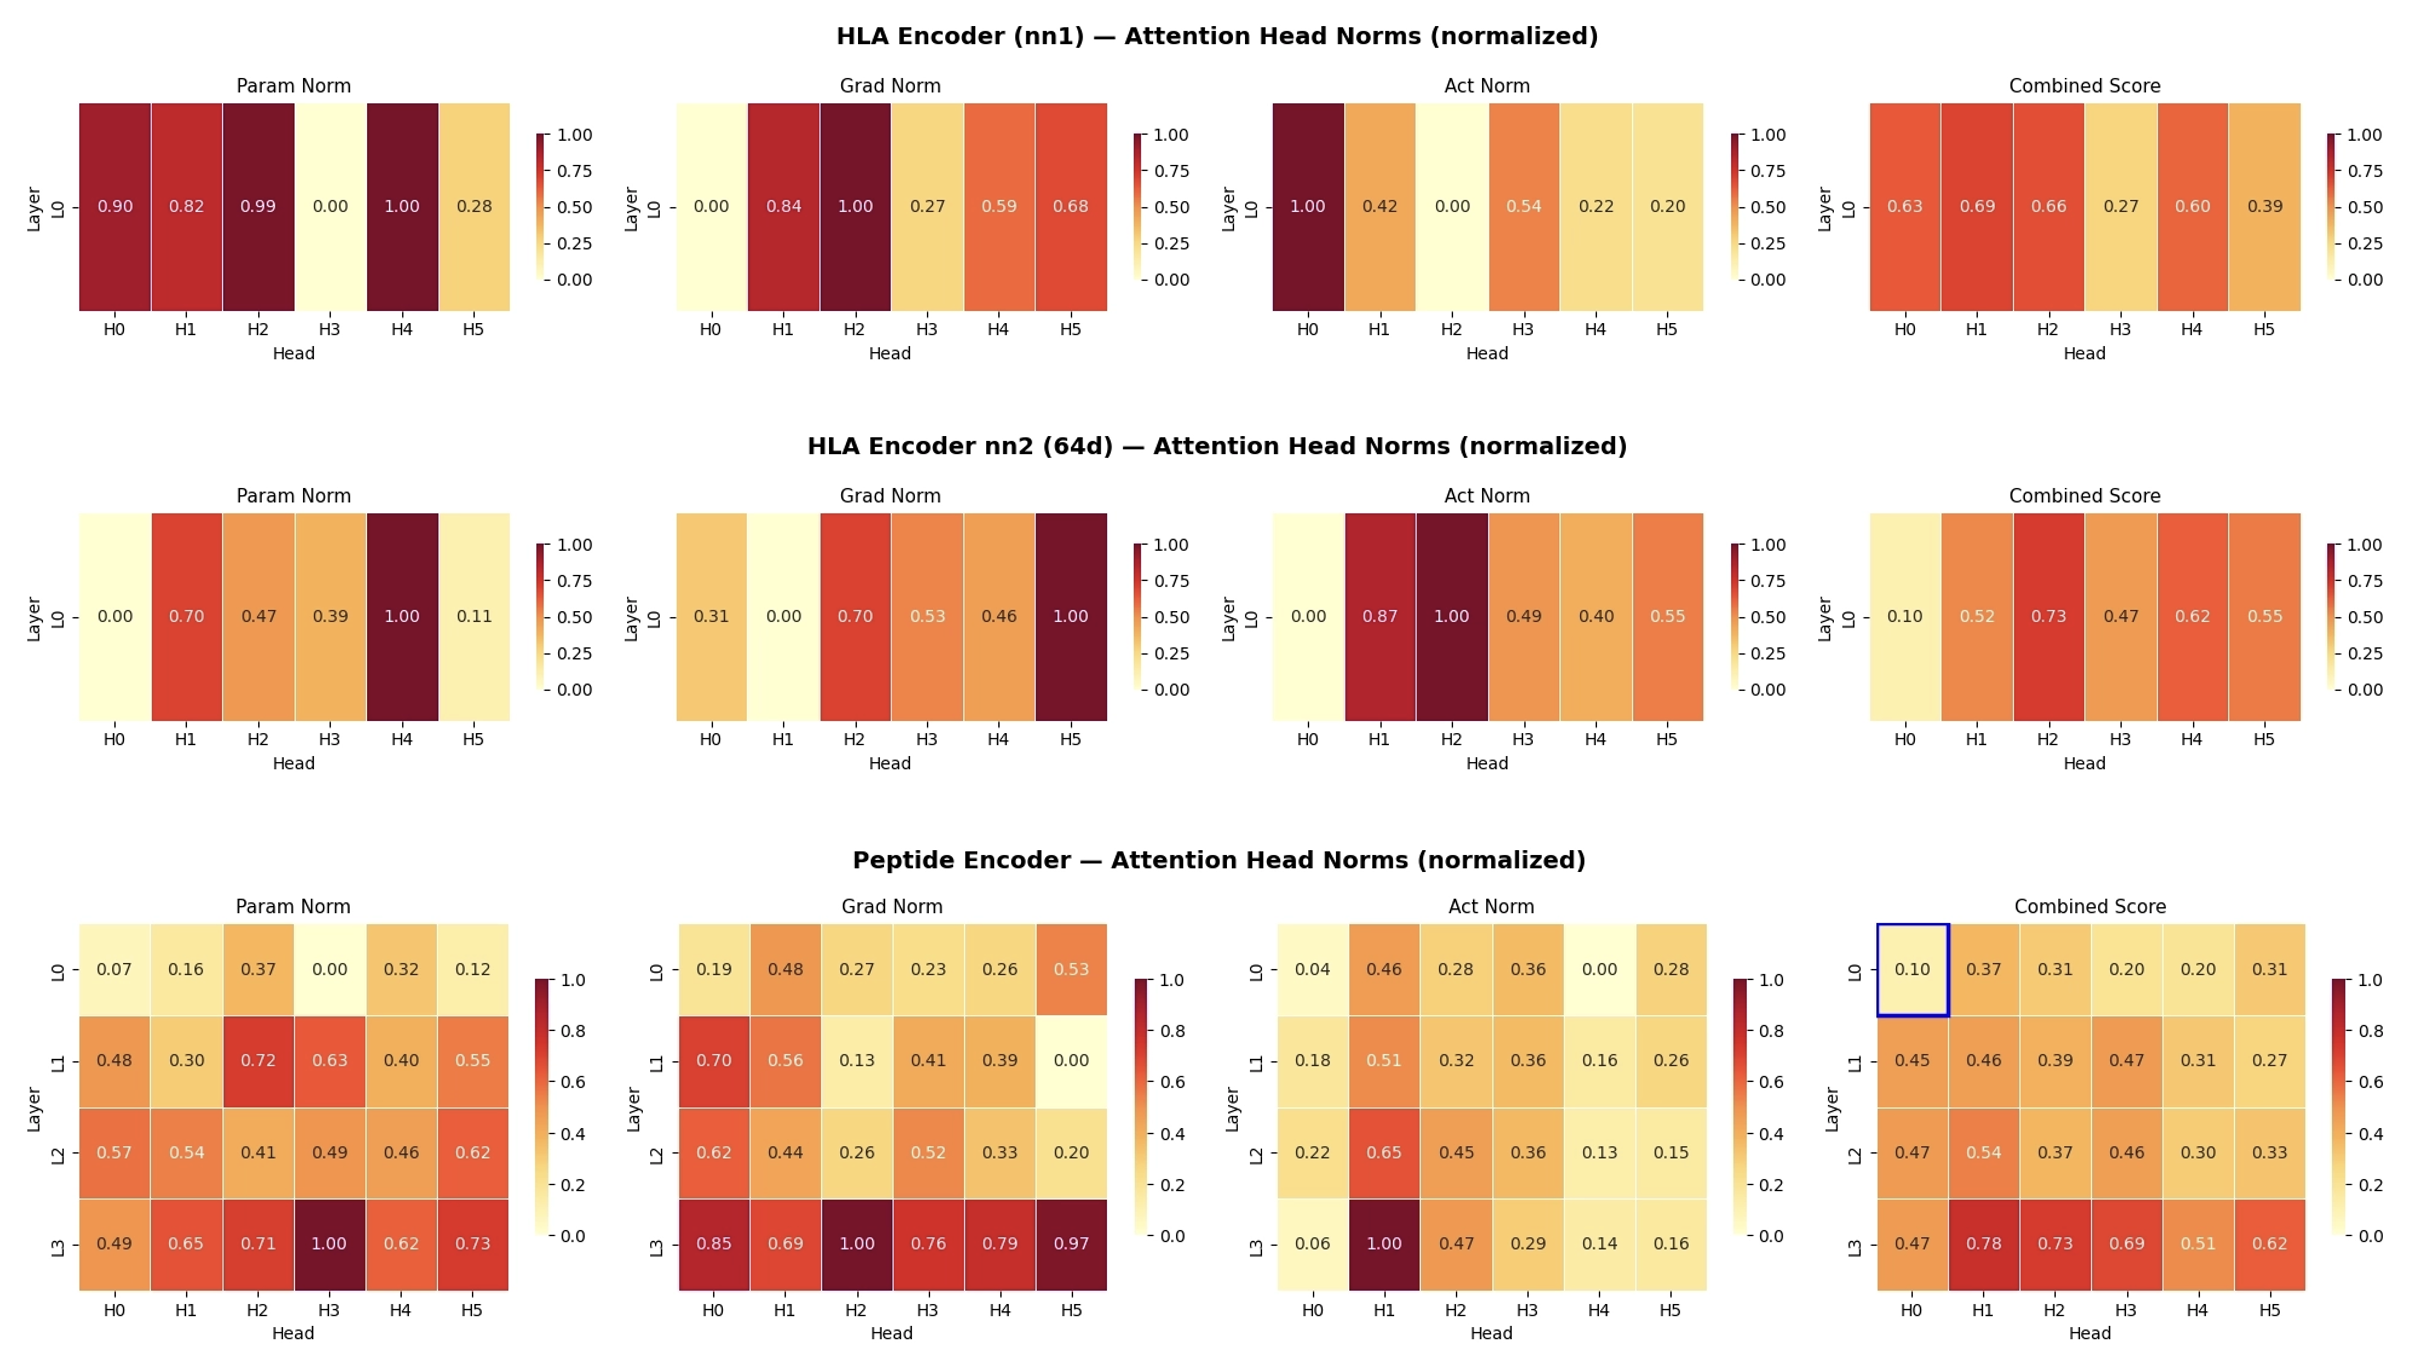
\includegraphics[width=1.0\textwidth]{figures/attention_head_importance.png}
    \caption{注意力头重要性热图}
    \label{fig:attention-head-importance}
\end{figure}

在 HLA Encoder 中，nn1 的 H0、H2、H3、H5 以及 nn2 的 H2、H4、H5、H3 贡献突出，应优先保留。在 Peptide Encoder 中，L0--H0 的 Combined Score 在全模型中最低，各类范数也普遍偏低，几乎未提供有效表征，因而被视为强剪枝候选；L0--H3 同样贡献偏弱，也可作为优先剪枝对象。与之相对，L3 中的 H1、H2、H3、H5 以及同层的 H0、H4 重要性较高，剪枝时应予以保留。

这些结果表明，FennOmix.MHC 的不同注意力头并非等价贡献，部分结构承担了主要表征功能，而另一些则贡献较弱，这为基于重要性分析的剪枝提供了实验依据。

\subsection{剪枝前后性能比较}

完成重要性分析后，本文对低贡献结构实施了剪枝，并测试了剪枝后模型的预测性能。由图~\ref{fig:pruning-performance} 可见，剪枝前后模型的整体性能差异较小，主要评价指标未出现显著下滑。

这一结果说明，当前模型结构中确有一部分可压缩的冗余。通过合理选择低重要性注意力头或前馈层进行剪枝，可以在基本保持模型预测能力的同时降低结构复杂度。对于后续部署而言，剪枝可作为降维之外的补充优化手段，进一步削减推理阶段的冗余计算。

\begin{figure}[htbp]
    \centering
    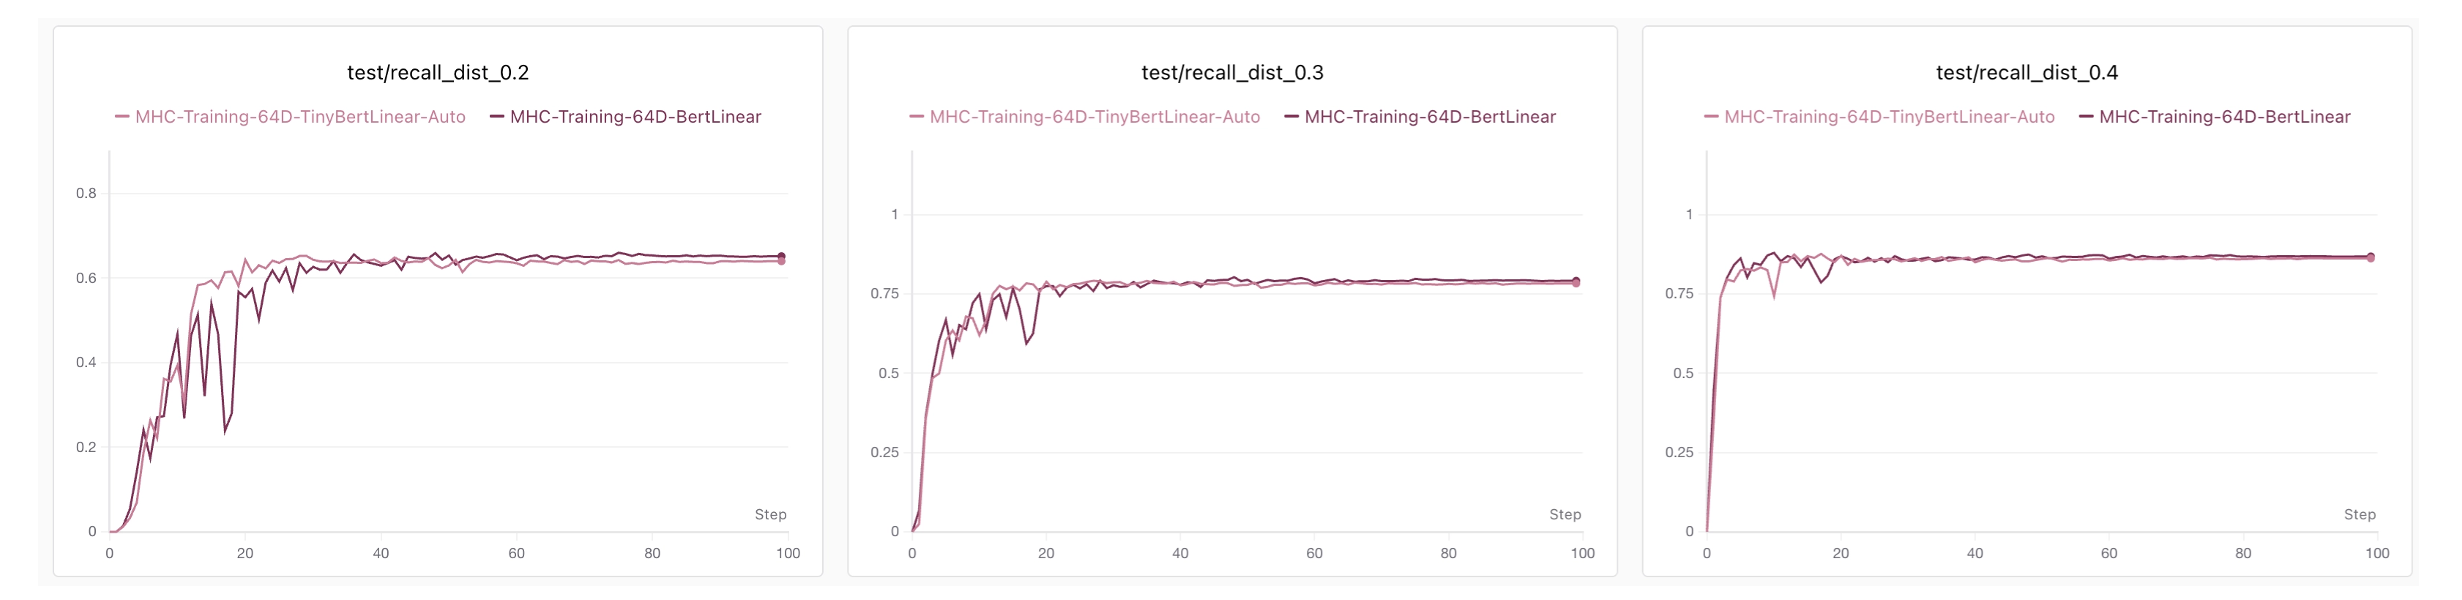
\includegraphics[width=1.0\textwidth]{figures/pruning_performance.png}
    \caption{模型剪枝前后性能对比图}
    \label{fig:pruning-performance}
\end{figure}

\subsection{剪枝结果讨论}

剪枝实验的主要价值并不在于显著提升预测性能，而在于证实模型结构仍有进一步压缩的空间。与输出维度压缩重点降低缓存成本不同，剪枝直接对模型结构做减法，有助于减少推理时的计算量。不过，目前的剪枝实验仍以验证可行性为主，对不同剪枝比例、组合策略以及剪枝后实际推理加速效果的分析还不够深入。因此，我们将剪枝结果定位为一种结构冗余的验证与部署优化的初步探索，为后续更细粒度的模型压缩研究提供基础。

\section{缓存压缩与索引机制实验分析}

\subsection{64 维缓存的压缩需求}

前面的实验已经表明，64D 模型可将肽段缓存从 132 GB 压缩至 19 GB，但在 7300 万条肽段的大规模场景下，19 GB 依然会带来一定的存储、加载和传输压力。因此，在 64D float32 缓存的基础上，我们进一步检验 INT8 量化压缩与索引加载策略的实际效果。本节重点从误差、存储收益和加载方式三个角度分析其部署表现。

\subsection{INT8 量化压缩结果}

从图~\ref{fig:quantization-result} 可以看出，采用 INT8 量化后，64D 肽段向量的主体数据由 float32 的 4 Byte/维压缩为 int8 的 1 Byte/维。忽略少量缩放因子与文件头开销后，embedding 主体数据的体积可近似缩减至原来的四分之一。

误差方面，量化后的实际 MSE 约为 $7.5 \times 10^{-7}$，低于理论最大值 $2.1 \times 10^{-6}$。这说明量化压缩虽然降低了存储位宽，但对向量数值分布的扰动非常轻微。后续匹配主要依赖 HLA 与肽段嵌入间的距离关系，如此低的量化误差意味着该方法具备较好的部署可行性。

\begin{figure}[htbp]
    \centering
    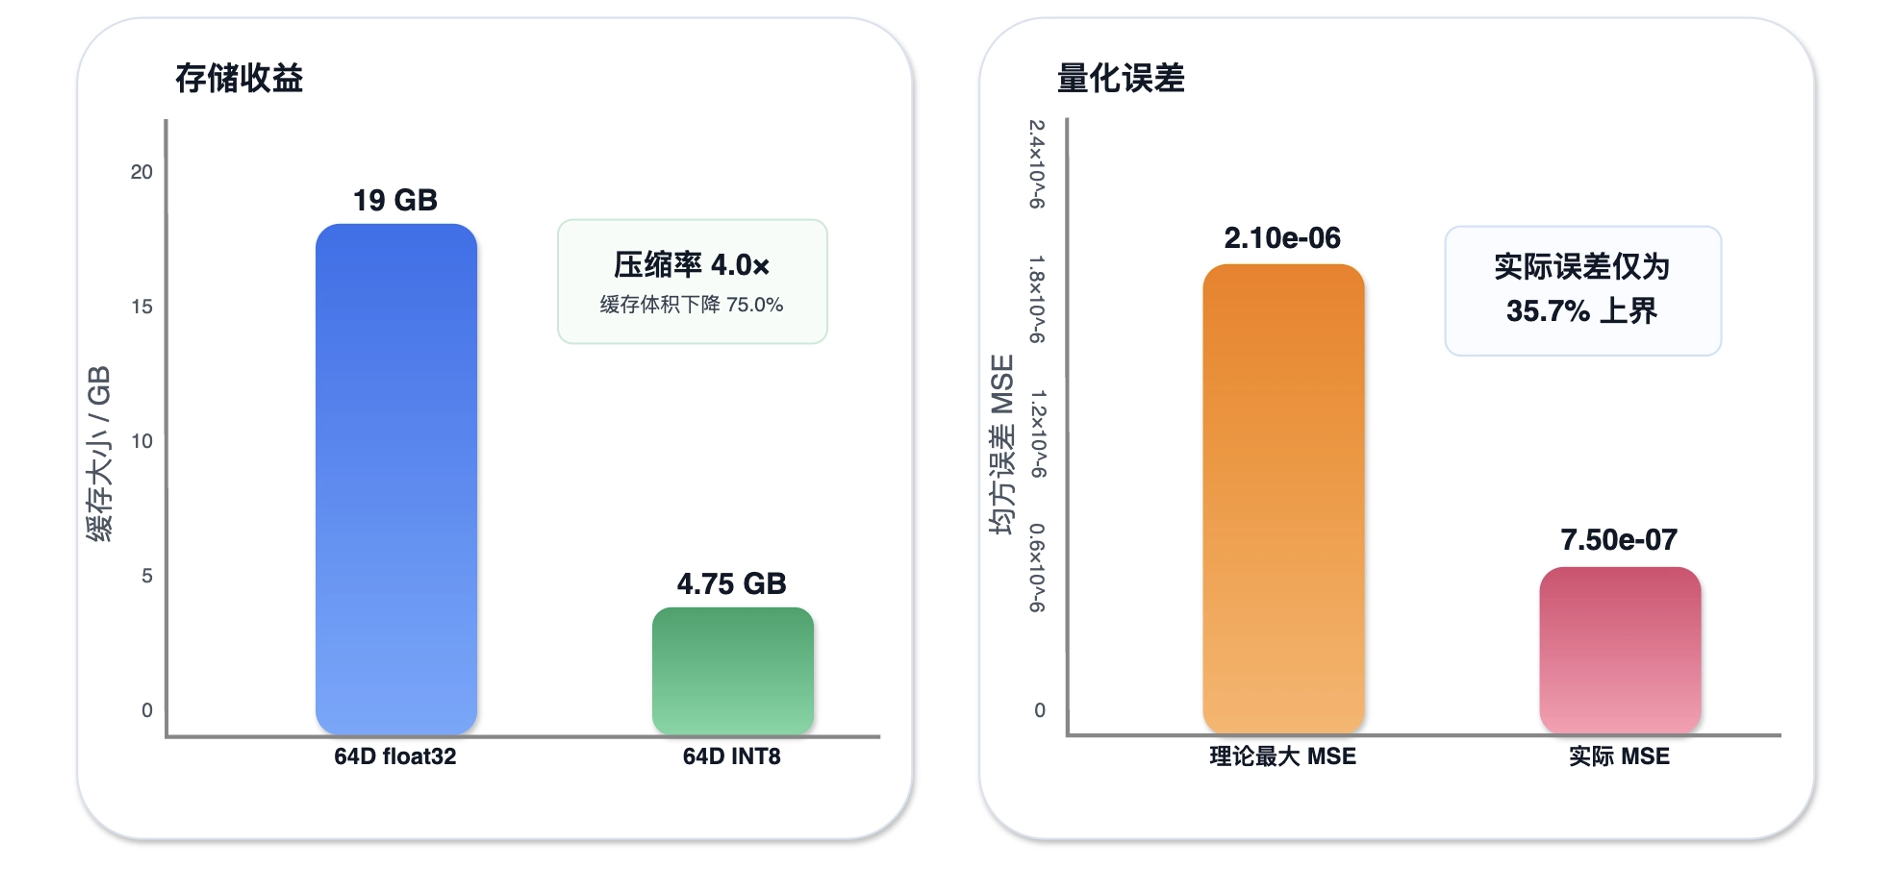
\includegraphics[width=0.80\textwidth]{figures/quantization_result.png}
    \caption{量化误差与存储收益图}
    \label{fig:quantization-result}
\end{figure}

综合来看，INT8 量化能在保持较高数值精度的同时进一步缩减缓存占用，是 64D 降维之后的一个重要补充优化。

\subsection{索引机制与加载策略分析}

\begin{figure}[htbp]
    \centering
    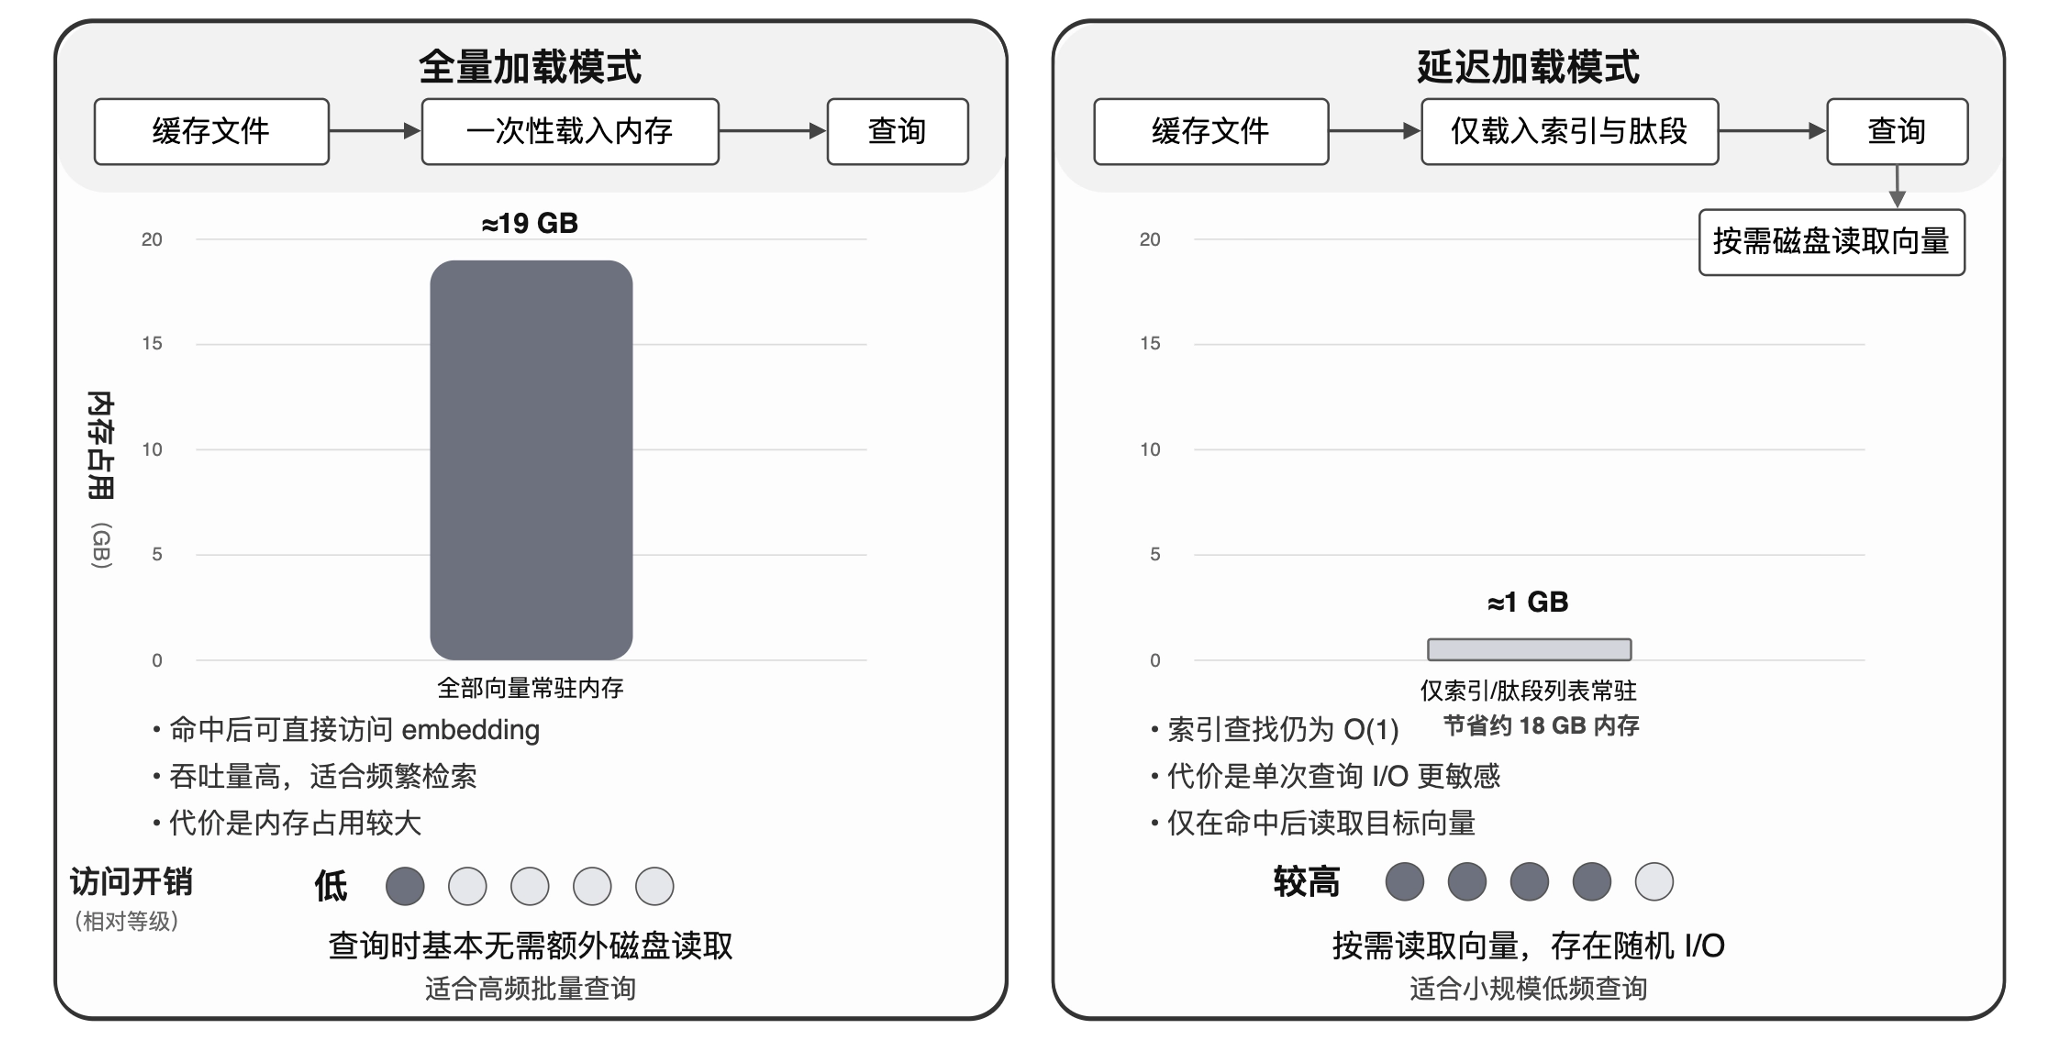
\includegraphics[width=0.80\textwidth]{figures/loading_strategy_result.png}
    \caption{全量加载与延迟加载的内存/访问开销分析图}
    \label{fig:loading-strategy-result}
\end{figure}

在索引机制层面，我们利用 peptide\_index 建立了肽段字符串到向量位置的映射，使系统在缓存命中时能够快速定位对应的嵌入向量。实验分析表明，这一设计可以避免在数千万级候选肽段中逐条搜索，让查询过程更适合大规模部署场景。

在加载策略层面，全量加载与延迟加载分别适配不同的资源条件。全量加载适合高频查询，能减少查询过程中的磁盘访问延迟；延迟加载则适合小规模查询或内存紧张的环境，仅加载肽段列表与索引，在需要时才读取对应向量。实验估算显示，延迟加载模式可节省约 18 GB 内存，能有效降低系统的常驻资源占用。

可以看出，索引与加载策略的价值不仅体现在查询速度上，也体现在部署灵活性上。系统可以根据任务规模、查询频率和硬件条件在全量加载与延迟加载之间灵活切换。

\subsection{查询链路效果分析}

在完整的查询链路中，系统优先通过索引判断输入肽段是否命中缓存：命中的肽段直接读取缓存向量，未命中的则回退到实时编码路径。随后，系统计算肽段 embedding 与目标 HLA embedding 之间的欧氏距离，并基于距离阈值或排序结果输出潜在结合肽段。

实验分析表明，这条链路能够兼顾高效性与开放性。常见的候选肽段可以受益于离线缓存和索引机制，减少重复编码开销；缓存外的新肽段则通过实时编码路径保证系统依然具备处理能力。从这个角度来看，缓存压缩与索引机制并不是孤立的优化，而是与在线预测流程共同构成了完整的部署链路。

\section{综合讨论}

\subsection{从模型精度到系统部署的统一优化路径}

本章实验结果揭示，本文所提的优化路线并非单层面的性能微调，而是从模型表示、模型结构和系统缓存三个层面逐步压低部署成本。

首先，在模型表示层面，64D 在保持 distance-recall 基本不变的前提下，将缓存规模从 132 GB 压缩至 19 GB，是当前性能与成本之间较理想的折中。其次，在降维模型选择上，Linear 与 MLP 的常规指标接近，而 Linear 在下游缩库辅助搜库任务中略占上风，故更适合作为默认方案。再次，在模型结构层面，剪枝实验揭示了模型内存在可压缩冗余，合理剪枝后性能依旧稳定。最后，在系统缓存层面，INT8 量化与索引加载机制进一步减轻了存储和内存压力，使模型更契合大规模候选肽段场景。

\subsection{实验结果的主要结论}

本章实验可归结出以下结论。第一，64D 是当前实验条件下较优的输出维度，其在 dist@0.3 和 dist@0.4 上几乎与 480D 持平，同时大幅压缩了缓存成本。第二，Linear 与 MLP 在常规预测指标上差异甚微，Linear 在下游缩库辅助搜库任务中整体略优且结构更轻量，因而更适宜作为默认降维模型。第三，剪枝实验表明 FennOmix.MHC 存在一定的结构冗余，基于重要性分析进行剪枝可在性能基本稳定的前提下降低模型复杂度。第四，INT8 量化能够进一步压缩 64D 缓存，实际 MSE 维持在较低水平；配合哈希索引和两阶段加载策略后，系统在存储、内存和访问方式上展现出更好的部署适应性。

\subsection{当前实验的局限性}

尽管本章实验验证了整体技术路线的可行性，但仍存在若干不足。首先，模型剪枝实验目前主要关注剪枝前后的性能稳定性，对不同剪枝比例、不同层级组合以及实际推理加速效果的分析尚待细化。其次，INT8 量化实验主要从误差角度论证了压缩效果，对于不同量化参数如何影响最终检索性能还可进一步探究。最后，索引与加载策略虽已完成原型验证，但在多进程、多机环境下的吞吐量、延迟和容错能力仍需更系统的测试。

因此，本文当前的实验更侧重于证明“降维—剪枝—缓存压缩—索引检索”这条路径的可行性，后续仍有必要围绕参数组合、速度收益和工程鲁棒性进行补充研究。

\section{本章小结}

本章围绕 FennOmix.MHC 的模型优化与系统部署需求，开展了系统的实验分析。首先，比较了 480D、128D、64D 和 32D 四种输出维度，结果显示 64D 在保持嵌入空间结构稳定的同时显著降低了缓存成本。其次，对比了 Linear 与 MLP 两类 64D 降维模型，发现二者常规指标接近，Linear 在下游缩库辅助搜库任务中略优，故被确定为默认降维方案。随后，剪枝实验证实模型结构中存在一定冗余，基于重要性分析的剪枝可在性能基本稳定的前提下减少模型复杂度。最后，INT8 量化、哈希索引与两阶段加载策略进一步提升了系统在大规模肽段库场景下的可部署性。

整体而言，本章的实验结果印证了本文所提优化路线的可行性与应用价值，也为第四章进一步展开系统设计与部署分析提供了实验依据。

\chapter{系统设计与部署分析}

\section{系统总体架构设计}

\begin{figure}[htbp]
    \centering
    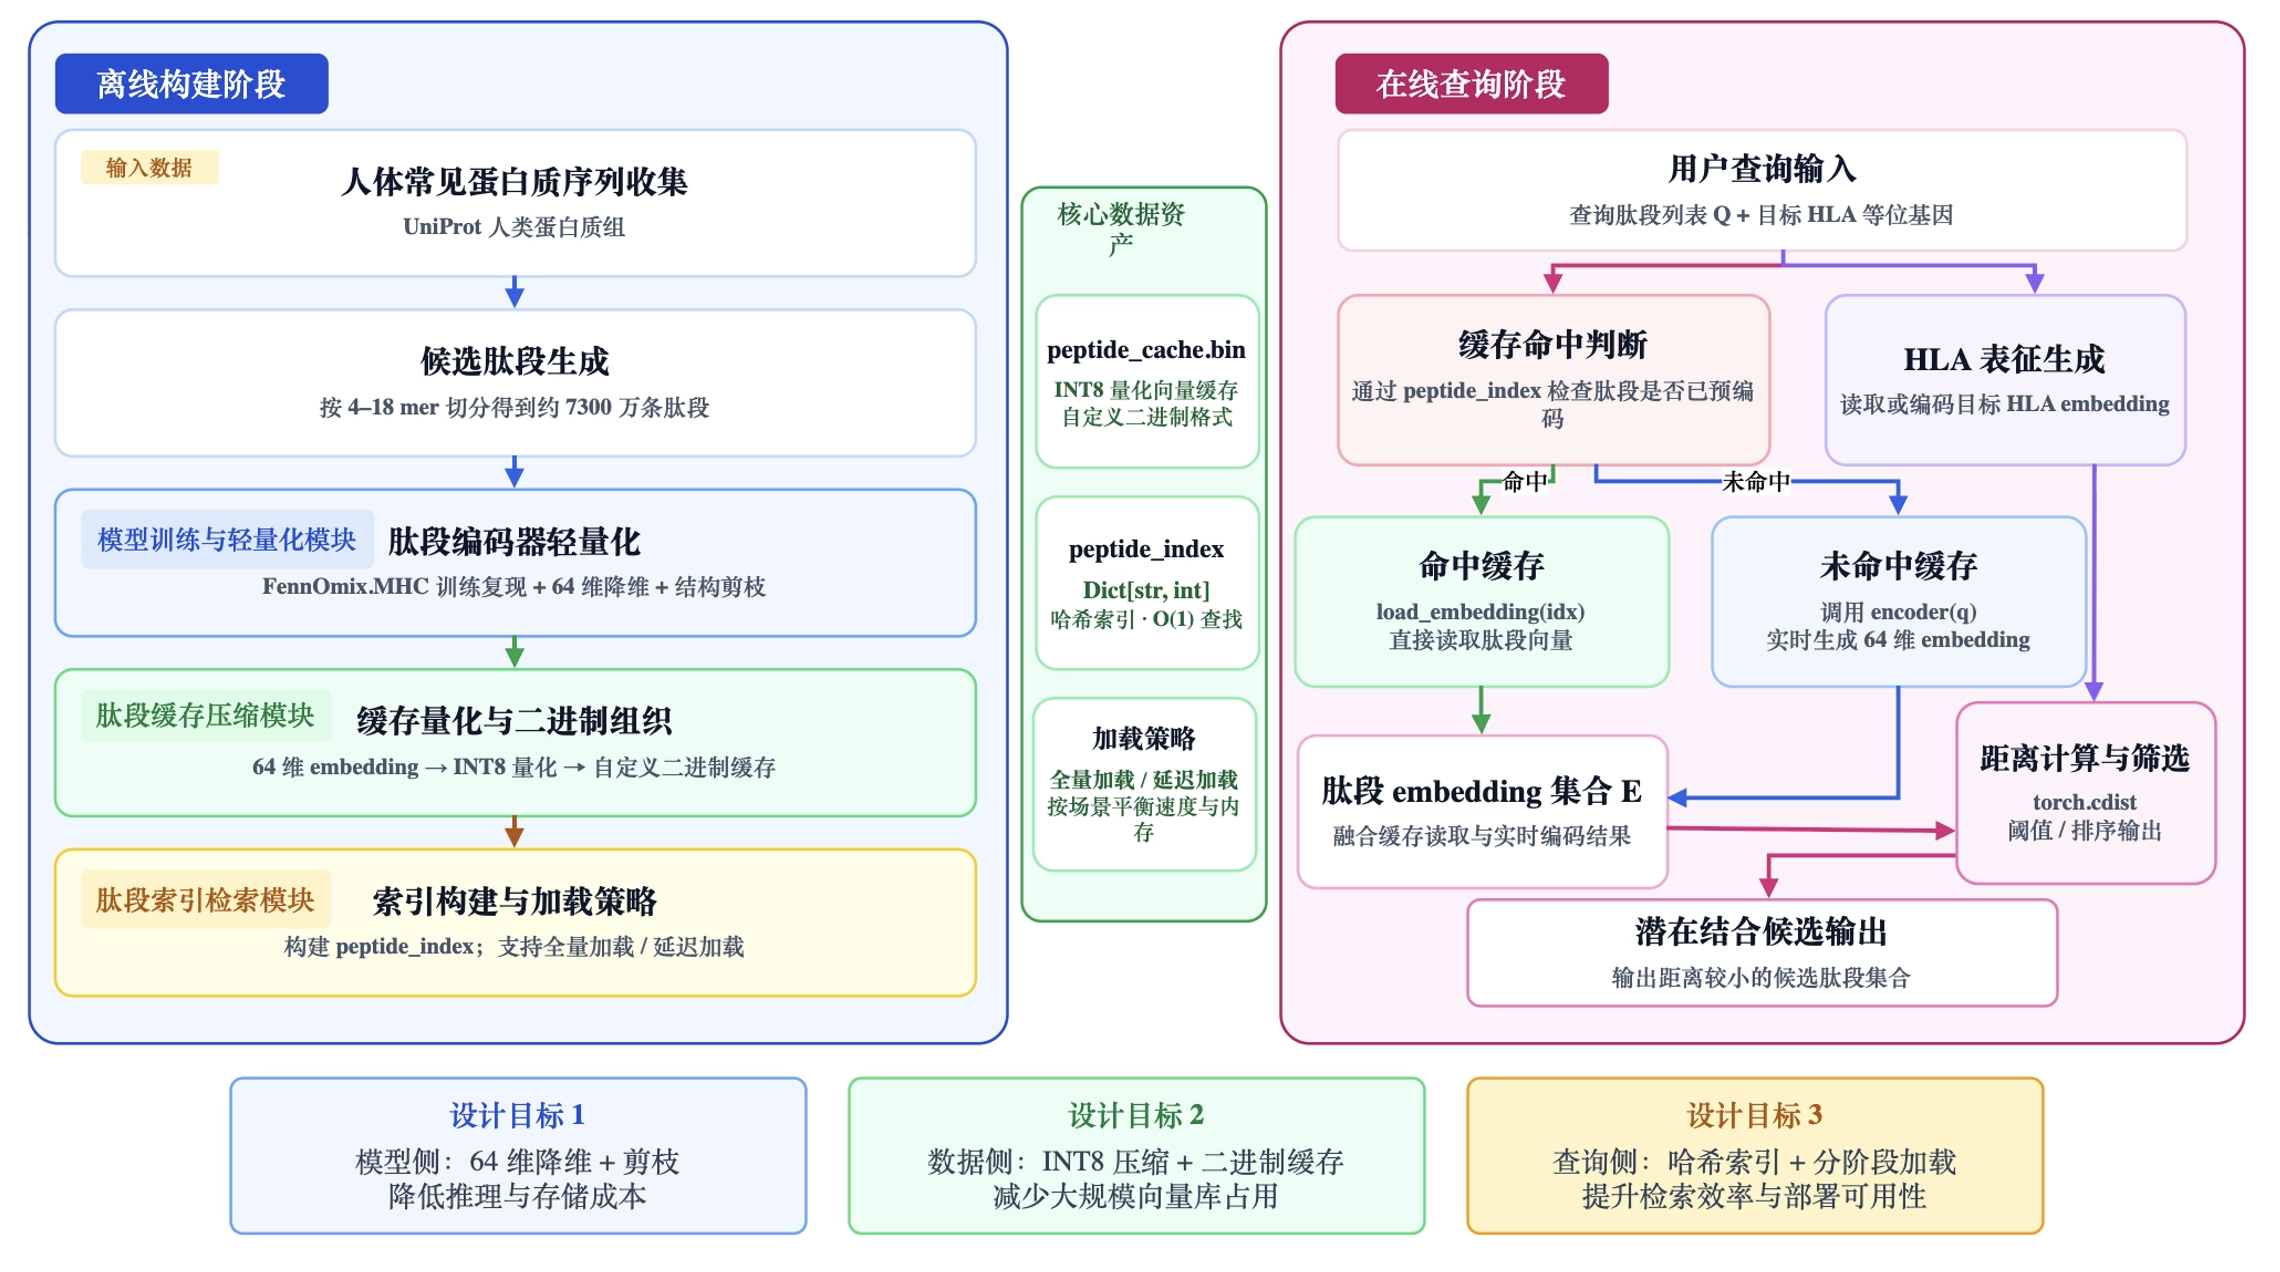
\includegraphics[width=0.95\textwidth]{figures/system_architecture.png}
    \caption{系统总体架构图}
    \label{fig:system-architecture}
\end{figure}

\subsection{系统设计目标}

前文已经从模型轻量化、缓存压缩和索引机制几个方面，验证了在大规模人类蛋白质组场景下优化 FennOmix.MHC 的可行性。本章不再重复具体实验结果，而是聚焦于系统实现与部署，说明这些优化如何被整合成一套可运行的预测和检索流程。

原始模型面对海量候选肽段时，最主要的困难在于在线编码和高维向量检索会带来极高的计算、存储和 I/O 成本。因此，本章系统设计的总体目标是：在保持预测能力的前提下，将模型优化的成果转化为可部署的工程链路，使其能够支撑离线缓存构建、在线快速查询，并在不同资源条件下灵活运行。

这一目标可以拆分为三点：用轻量化模型降低向量生成和推理阶段的计算开销；靠压缩缓存和索引结构压低海量肽段库的存储和访问成本；通过多种加载策略兼顾高频查询和资源受限两类部署场景。于是，本文的系统不再是孤立的模型，而是由模型、缓存、索引和在线查询流程共同组成的一条完整部署链路。

\subsection{离线构建与在线查询流程}

从运行阶段来看，系统可分为离线构建和在线查询两部分。

离线构建阶段负责处理计算量大、但执行频率低的工作。这一步先将候选蛋白序列切割成候选肽段集合，再调用训练好的轻量化肽段编码器生成肽段向量，随后把这些向量写入压缩缓存文件，并同步建立肽段序列到缓存位置的索引映射。目的就是把大批量重复计算前移，为在线查询准备好可复用的数据基础。

在线查询阶段承担实时响应任务。系统拿到输入肽段和目标 HLA 信息后，先通过索引判断该肽段是否已在缓存中：命中则直接读取向量，未命中则调用轻量化编码器实时生成向量。之后，根据肽段向量与 HLA 向量之间的距离关系，给出潜在结合候选。

这种“离线预处理 + 在线快速调用”的划分，有效削减了在线阶段重复推理的开销，使系统在大规模候选库条件下具有更好的响应能力。

\subsection{系统模块划分}

为了便于实现、维护和扩展，系统被拆分为四个核心模块：模型训练与轻量化、肽段缓存压缩、肽段索引检索以及在线预测执行。各模块的功能见表~\ref{tab:system-modules}。

\begin{table}[htbp]
    \centering
    \caption{系统核心模块划分}
    \label{tab:system-modules}
    \begin{tabular}{p{0.24\textwidth} p{0.36\textwidth} p{0.30\textwidth}}
        \toprule
        模块 & 主要功能 & 在系统中的作用 \\
        \midrule
        模型训练与轻量化模块
        & 模型复现、64D 降维、Linear 模型选择与结构剪枝
        & 提供轻量化编码器 \\

        肽段缓存压缩模块
        & 生成并存储压缩后的肽段向量缓存
        & 缓解大规模缓存的存储压力 \\

        肽段索引检索模块
        & 构建肽段到缓存位置的映射，支撑多种加载方式
        & 提升查询定位效率 \\

        在线预测执行模块
        & 执行输入处理、缓存读取、实时编码与距离计算
        & 构成完整的预测服务流程 \\
        \bottomrule
    \end{tabular}
\end{table}

通过这样的划分，模型计算、缓存存储、索引定位和在线预测被解耦成相对独立的功能单元，既降低了耦合度，也为日后单独替换或改进某个模块留下空间。

\section{关键模块实现与协同流程}

\begin{figure}[htbp]
    \centering
    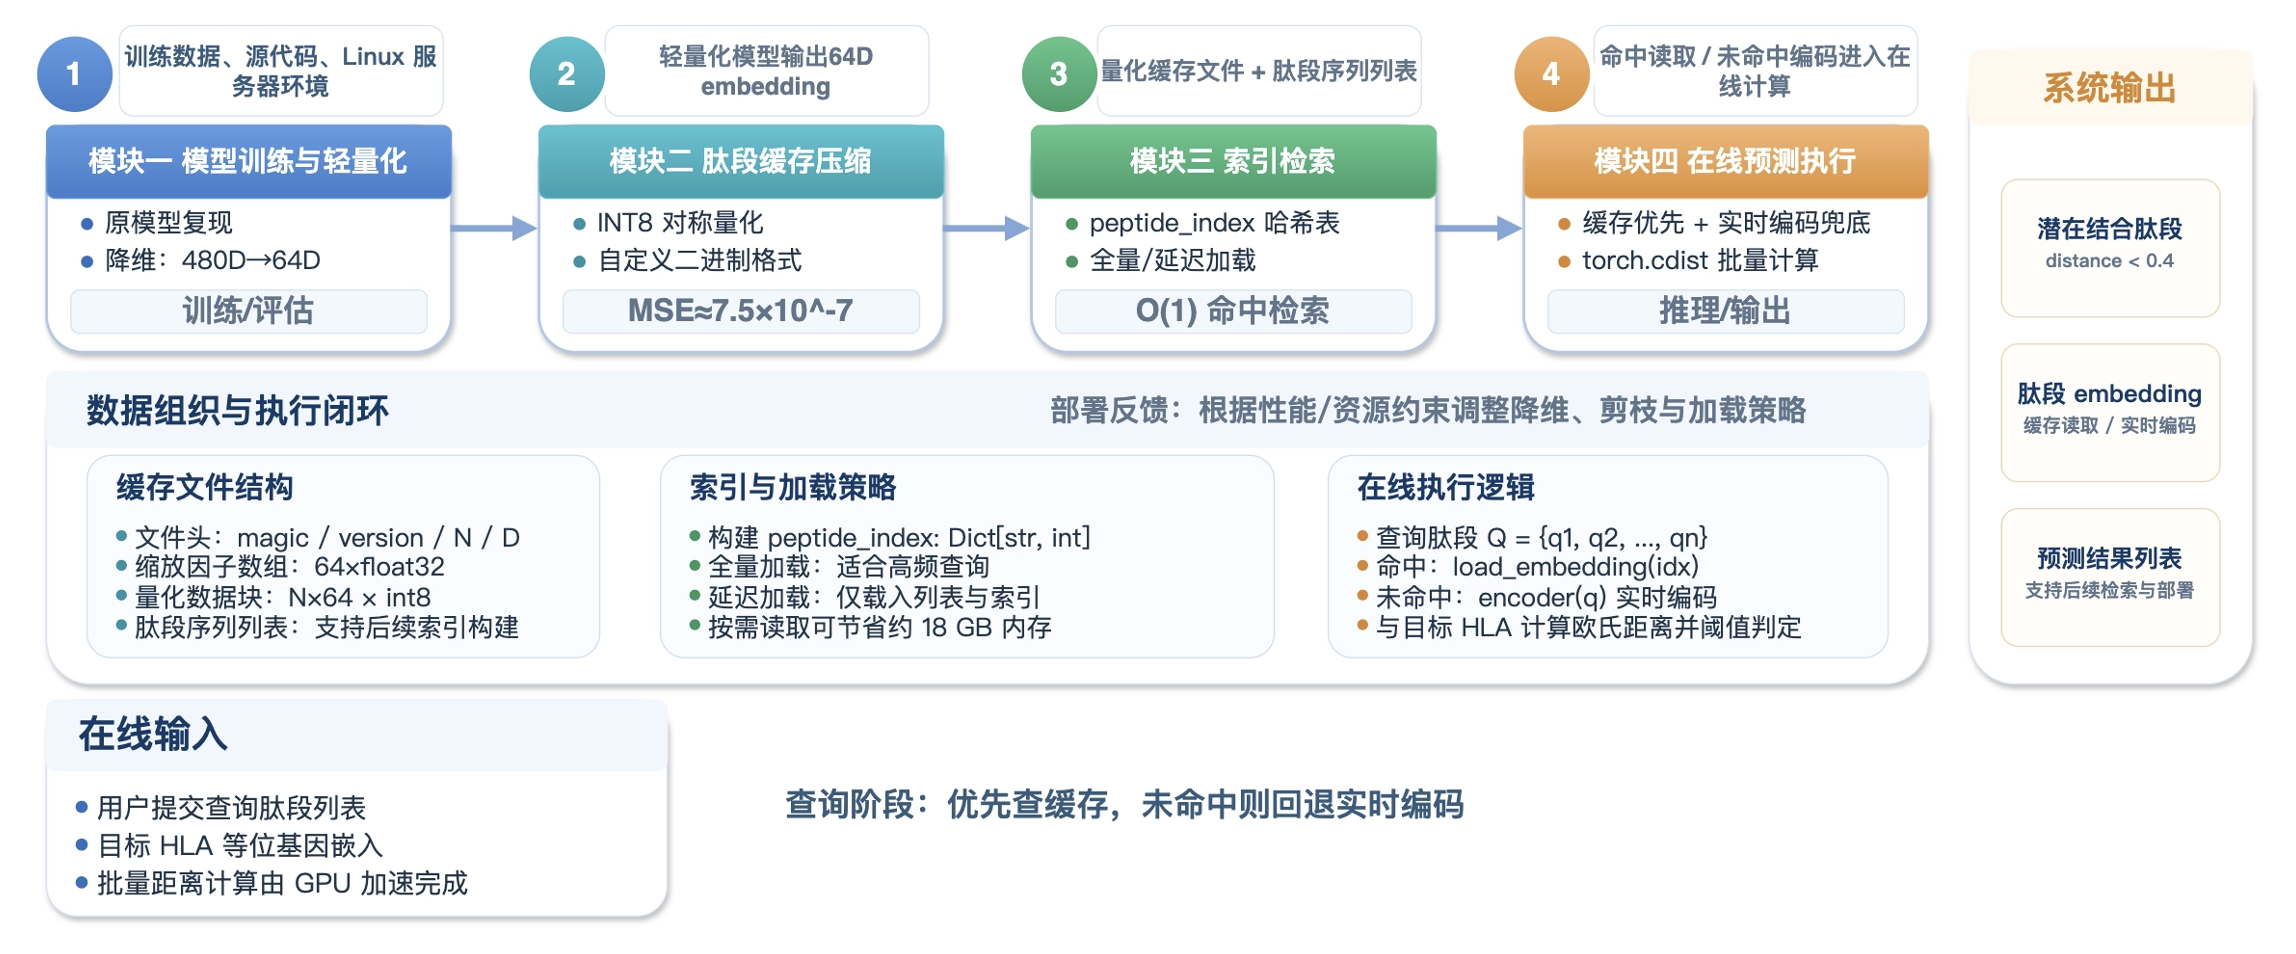
\includegraphics[width=0.95\textwidth]{figures/module_workflow.png}
    \caption{各模块协同流程图}
    \label{fig:module-workflow}
\end{figure}

\subsection{模型训练与轻量化模块}

该模块是整个系统的基础，负责输出可以实际部署的编码器。我们在 FennOmix.MHC 原始框架上完成了模型复现，并根据前面的实验结果选定了适合部署的轻量化配置。

在系统中，这一模块承担两项工作：一是在离线阶段批量生成候选肽段向量，为后续缓存构建提供原料；二是在在线阶段处理缓存未命中的新肽段，保证系统不会完全受限于固定的候选库。

模块的输出包括模型权重文件、配置文件和必要的推理接口。为防止不同实验版本混淆，系统对模型文件命名、参数记录和缓存版本三者之间维持了严格的对应关系。只有模型版本、缓存文件和索引文件保持一致，在线查询结果才能具备可追溯性和可复现性。

\subsection{肽段缓存压缩模块实现}

肽段缓存压缩模块负责将离线生成的大规模 peptide embedding 转换成更利于部署的存储形式。第二章已详细介绍过 INT8 量化方法和自定义二进制格式，这里不再重述具体机制，而是把重点放在该模块在系统中的实现作用上。

在系统流程中，该模块接收轻量化肽段编码器生成的 64D float32 向量，输出压缩后的缓存文件。文件中保存了必要的元信息、量化参数、压缩向量数据和肽段序列信息，供后续索引模块读取和定位。实验结果显示，INT8 压缩后的实际 MSE 约为 $7.5 \times 10^{-7}$，表明该模块在压缩存储占用的同时，对向量数值分布的扰动非常有限。

从部署角度看，缓存压缩模块的价值主要体现在三处：缩减磁盘存储占用；降低缓存文件在不同环境间迁移和备份的成本；为后续索引加载和在线查询提供更紧凑的数据基础。

\subsection{肽段索引检索模块实现}

肽段索引检索模块在查询肽段和缓存向量位置之间建立映射关系。它读取缓存文件中的肽段序列信息，生成可供在线查询使用的索引结构。

在线运行期间，索引模块先判断输入肽段是否在缓存中：命中则返回对应的缓存位置，缺失则将该肽段转交给在线编码模块处理。通过这一机制，系统优先复用离线缓存的成果，并在必要时回退到实时推理路径。

\subsection{在线预测执行模块实现}

在线预测执行模块是系统面向用户或下游任务的核心执行单元，它将轻量化模型、缓存文件和索引结构串联起来，形成完整的预测流程。

系统收到查询肽段和目标 HLA 信息后，先由索引模块判定缓存是否命中。命中的肽段直接读取缓存向量，未命中的则调用轻量化编码器实时生成 embedding。随后，系统对获得的肽段向量与目标 HLA 嵌入进行距离计算，并依据距离阈值或排序结果输出潜在结合肽段。

\subsection{模块协同关系}

四个模块的协同关系可以概括为：模型训练与轻量化模块提供编码器，缓存压缩模块基于该编码器生成压缩缓存，索引检索模块在缓存文件之上建立快速定位能力，在线预测执行模块则统一调度编码器、缓存和索引来完成最终预测。

这种协同方式有两方面好处：离线阶段和在线阶段职责分明，减少了在线服务中的重复计算；各模块接口相对独立，便于后续单独优化某一环节，比如更换量化方式、调整加载策略或改进在线预测接口。

\section{部署模式与资源开销分析}

\subsection{单机部署模式分析}

当前系统原型主要面向单机部署环境，好处是结构简单、调试方便。系统运行所需的资源主要是 GPU 显存、主机内存和磁盘空间。

GPU 主要用于模型实时编码和批量距离计算；主机内存用于加载索引结构以及部分或全部缓存数据；磁盘则保存大规模肽段缓存文件和模型权重文件。由于大量肽段编码工作已被迁移到离线阶段，在线阶段的计算压力主要集中在缓存读取、少量实时编码以及距离计算上。

在单机环境中，部署的关键不是片面追求模型性能，而是合理规划模型、缓存和索引的加载方式，让它们在有限的硬件资源下稳定运行。

\subsection{部署设计意义}

本文系统的意义并不仅仅在于提升某个单一的实验指标，更在于将原本难以部署的大规模高维 embedding 检索任务，逐步转化为一套可压缩、可索引、可按需加载、可在线查询的完整系统流程。

\section{本章小结}

本章从系统实现与部署的角度，分析了我们所提出的轻量化预测与检索方案。与侧重实验数据的前文不同，本章的关注点在于各优化模块如何组合成一个可运行的系统。

我们首先将系统划分为离线构建和在线查询两个阶段，确立了“离线预处理、在线快速调用”的总体思路。接着，进一步将系统拆解为模型训练与轻量化、肽段缓存管理、肽段索引检索和在线预测执行四个模块，并说明了各自的输入、输出和协同关系。然后，结合单机部署场景，讨论了全量加载与延迟加载两类部署模式的适用条件。最后，从工程实现特点、可复现性保障和当前工程难点三个维度，探讨了系统后续的完善方向。

整体来看，本文系统已从单一的模型优化，拓展为“轻量化模型—压缩缓存—索引检索—在线预测”这样一条完整的部署链路，为 FennOmix.MHC 在大规模人类蛋白质组场景中的实际应用提供了系统化的支撑。

\chapter{总结与展望}

\section{全文总结}

本文围绕深度学习免疫多肽结合预测模型的优化与部署展开，以 FennOmix.MHC 为基础，针对其在大规模人类蛋白质组应用中暴露出的高维表示、缓存膨胀、I/O 负担重和部署代价高等问题，从模型轻量化和系统工程优化两个方向进行了探索。

在模型优化方面，我们首先复现了 FennOmix.MHC，随后依次尝试了输出维度压缩、降维结构对比和模型剪枝。实验表明，适度压缩嵌入维度能够在守住核心预测能力的同时，大幅削减缓存规模；对比线性与非线性降维方案后，线性结构在性能、简洁性和下游任务表现之间取得了更均衡的效果；剪枝实验则揭示了模型内部存在冗余，经合理裁剪后模型表现依然稳健。

在系统优化方面，我们针对大规模肽段缓存的存储与访问难题，设计了缓存压缩、索引定位和分阶段加载机制。通过将离线预计算、压缩缓存、哈希索引和在线查询整合为一条完整的优化链路，有效降低了重复编码开销，缓解了缓存存储压力，提升了模型在大规模候选肽段筛选场景中的可用性。

总体来看，我们并没有孤立地追求单一指标的提升，而是紧扣 FennOmix.MHC 的实际部署需求，对模型表示压缩、结构优化、缓存管理和索引检索进行了统一设计。结果表明，面向大规模候选库的免疫多肽结合预测模型，在关注预测精度的同时，必须一并考量存储成本、访问效率和运行环境等工程因素。本文的工作验证了这一优化思路的可行性，并为后续系统的迭代改进提供了参考。

\section{本文工作不足}

尽管围绕模型轻量化与部署优化开展了较系统的研究，当前工作仍存在若干局限。实验设计更侧重验证整体技术路线的可行性，对部分参数组合的探索尚欠充分：剪枝部分已证实基于重要性分析的策略可行，但不同剪枝比例、层级组合以及剪枝后推理速度变化的系统比较仍需细化；缓存压缩方面，虽从误差角度验证了方法的有效性，而不同量化参数对检索结果及系统延迟的影响仍有待深入剖析。此外，系统虽已串接为原型链路，但工程完备性尚有提升空间。模型、缓存、索引与在线查询之间的多模块协同对数据格式、版本管理和接口一致性提出了较高要求，在大规模离线构建或多进程运行场景下，还需补充任务调度、断点续算、异常处理和日志记录等功能。最后，部署分析主要依托单机环境与原型验证，对不同硬件条件、查询负载及高并发场景的性能表现仍缺少更充分的测试，因此当前成果更适合定位为方法验证与系统原型基础，距离成熟稳定的实际应用系统仍有完善余地。

\section{后续研究展望}

针对上述不足，未来工作可从以下几个方向推进。其一，细化模型轻量化策略：在降维方面，继续探索更契合免疫多肽结合预测特性的压缩结构和低位宽表示；在剪枝方面，系统比较不同剪枝比例、位置与组合对模型性能、参数量及推理速度的影响，以形成更为可控的模型压缩方案。其二，完善缓存压缩与索引系统的工程实现：在现有原型上补充缓存一致性校验、异常处理、日志管理与自动化构建流程，并测试不同查询规模下全量加载与延迟加载两种模式的实际表现，使部署分析更为完整。其三，拓展技术路线的适用边界：本文凝练的“模型轻量化 + 缓存压缩 + 索引检索”思路并不局限于 FennOmix.MHC，也可为其他面向大规模候选库筛选的生物信息学深度学习模型提供借鉴。随着蛋白质语言模型、对比学习与向量检索技术在生命科学中的不断渗透，如何在维持表示能力的同时压低系统部署成本，将成为值得持续探究的议题。

\section{本章小结}

本章归纳了全文的研究工作，并剖析了当前存在的不足与后续优化方向。概括而言，本研究瞄准 FennOmix.MHC 在大规模人类蛋白质组场景中的部署瓶颈，完成了模型轻量化、缓存压缩与索引检索等环节的探索，验证了模型优化与系统部署协同设计的可行性。未来仍需在参数精细化、工程鲁棒性提升及多场景部署测试等方面持续完善。


\end{document}
